\documentclass[english]{sintr}

% Document metadata
\articletype{Final Project Report}
\articleshorttile{Adaptive Learning and Path-Planning Engine}
% \authorheader{Bhuvan Chandra K}
\submitted{14 November 2026; revised 20 November 2026}

\newcommand{\abscontent}{}

\title{Adaptive Learning, Diagnostic Assessment and Personalized Path-Planning Engine -- Final Report}
\author{Bhuvan Chandra -- AI23BTECH11013, Abdur Rehman -- AI23BTECH11015 \\ Project 03 $\cdot$ Group 11 $\cdot$ CS5903 Distributed AI Training}

% --------------------------------------------------
% Packages
% --------------------------------------------------

% Figures and placement
\usepackage{graphicx}
\usepackage{float}

% Tables
\usepackage{longtable}
\usepackage{array}
\usepackage{booktabs}
\usepackage{tabularx}
\usepackage{multirow}

% Mathematics
\usepackage{amsmath}
\usepackage{amssymb}

% Lists and text formatting
\usepackage{enumitem}
\setlist{itemsep=1pt,topsep=3pt}

% Links and references
\usepackage{hyperref}
\hypersetup{colorlinks=true,linkcolor=blue!50!black,urlcolor=blue!50!black,citecolor=blue!50!black}

% --------------------------------------------------
% Custom column types for tables
% --------------------------------------------------
\newcolumntype{L}[1]{>{\raggedright\arraybackslash}p{#1}}
\newcolumntype{C}[1]{>{\centering\arraybackslash}p{#1}}
\newcolumntype{R}[1]{>{\raggedleft\arraybackslash}p{#1}}
% The submission guide numbers the ten required sections 1-10 (the Mid-Review used A-E).
\renewcommand{\thesection}{\arabic{section}}
\renewcommand{\thesubsection}{\thesection.\arabic{subsection}}

% --------------------------------------------------
% Evidence links: every file link points at the final tag
% --------------------------------------------------
\newcommand{\repourl}{https://github.com/Bhuvan-56/adaptive-learning-path-planner-DAT}
\newcommand{\sha}{cs5903-final-2026}
\DeclareRobustCommand{\rf}[1]{\href{\repourl/blob/\sha/#1}{\nolinkurl{#1}}}
\DeclareRobustCommand{\rd}[1]{\href{\repourl/tree/\sha/#1}{\nolinkurl{#1}}}
\DeclareRobustCommand{\cm}[1]{\href{\repourl/commit/#1}{\texttt{#1}}}
% Files added by the Week 8 public-data extension and demo pages (20 Nov 2026) exist only from this revision on.
\newcommand{\shax}{cs5903-final-2026}
\DeclareRobustCommand{\rfx}[1]{\href{\repourl/blob/\shax/#1}{\nolinkurl{#1}}}
\DeclareRobustCommand{\rfm}[1]{\href{\repourl/blob/\sha/#1}{\nolinkurl{#1}}}
\DeclareRobustCommand{\rdx}[1]{\href{\repourl/tree/\shax/#1}{\nolinkurl{#1}}}
\newcommand{\siteurl}{https://bhuvan-56.github.io/adaptive-learning-path-planner-DAT/site/}
\newcommand{\nd}{\textit{n.d.}}
\setlength{\emergencystretch}{3em}

\begin{document}
\maketitle

\noindent\begin{tabular}{@{}L{3.48cm}L{11.98cm}@{}}
\textbf{GitHub repository} & \href{\repourl}{adaptive-learning-path-planner-DAT} \\
\textbf{Final revision} & Tag \texttt{cs5903-final-2026} on branch \texttt{main}, the commit that adds this report; every file link in this report points at that tag \\
\textbf{Website and demo} & \href{\siteurl}{\nolinkurl{bhuvan-56.github.io/adaptive-learning-path-planner-DAT/site/}} \\
\end{tabular}

\subsection*{Executive Summary}
\textbf{Problem.} Learners differ in prior knowledge, target, deadline and daily time (5--30 min). A fixed course order cannot serve a beginner with 10 minutes a day and an experienced learner who wants a short refresher. The brief asks for an engine that estimates mastery with uncertainty, respects mandatory prerequisites, plans day by day within a time budget, adapts difficulty, schedules review and remediation, replans after missed work or changed constraints, and explains every decision, without private learner data.
\vspace{0.2em}\newline
\textbf{What we built.} A Python backend service with eight modules (M1--M8): a validated curriculum DAG; Bayesian Knowledge Tracing (BKT) mastery with an evidence-count uncertainty proxy and a four-state classifier; a 10-item computerized adaptive test (2PL IRT); a prerequisite-safe, budget-bounded daily planner with feasibility proofs and event-driven replanning; a 2-up/1-down difficulty staircase; Half-Life Regression review weighted by prerequisite importance, plus remediation; a machine-checked audit trace; and a closed-loop evaluation harness with synthetic learners. A static website with live in-browser demos runs the same Python code, plus two pages where a person or a simulated learner answers questions and the engine diagnoses and replans after every answer (Section~\ref{sec:ui}). BKT was also fitted on the public ASSISTments 2009--2010 dataset and tested on held-out students (Section~\ref{sec:public}).
\vspace{0.2em}\newline
\textbf{Results.} 21 acceptance groups: 20 pass, 1 partial (M4-a, agreed with the mentor); the recorded suite is 303 passed (299 on 14 November, plus 4 S4 tests). Across 45,000 simulated learner-runs there are 0 prerequisite and 0 budget violations, and trace coverage is 100\% for the primary arms. The adaptive arm beats the static prerequisite-order baseline in all five scenarios, by $+0.045$ to $+0.727$ concepts mastered (paired 95\% CIs above zero), and improves retained recall everywhere. Greedy scheduling reaches 0.974 of the exact optimum on average (0.981 with the best-singleton fallback). The CAT is more accurate than fixed or random items in 5 of 6 paired comparisons. On 593 held-out ASSISTments students, BKT fitted per skill predicts answers with AUC 0.714 (engine defaults 0.681, per-skill average 0.621), and on simulated learners calibrated to those fits (S4) adaptive still beats static, $+0.055$ [0.027, 0.083] concepts.
\vspace{0.2em}\newline
\textbf{Limits.} All planning outcomes are simulator behaviour on simulated learners; no real learner used the planner, and real data enters only through the ASSISTments fit and S4. Since the diagnostic was connected to the planner (Week 8), a cold-start ablation beats the full system on mastery in all five runs (Section~\ref{sec:failures}); remediation never triggers inside the closed loop; and planned reviews were logged as done, so a later replan could drop them (B14, found and fixed on 20 November; re-running all six integrated scenarios changed mean mastery by at most 0.002 concepts).
\newpage
\tableofcontents
\newpage

% ==================================================
\section{Problem, Scope and Success Criteria}
% ==================================================
\subsection{Problem Statement}
Given a curriculum of concepts with prerequisites, a learner's answers so far, a target concept, a deadline and a daily study budget, the engine must decide each day which lessons, exercises, reviews and remediation to schedule. The plan must never place a concept before its mandatory prerequisites are actually learned, must fit the day's minutes, must change when new evidence arrives or the learner misses work, and must say why every concept was included or left out. 
\subsection{Actors and Boundary}
{\small
\begin{longtable}{|L{3.14cm}|L{6.09cm}|L{5.80cm}|}
\caption{Actors and their interaction with the engine (\rf{docs/PROBLEM_BOUNDARY.md}).}\\
\hline
\textbf{Actor} & \textbf{Role} & \textbf{Interface} \\ \hline
\endfirsthead
\hline \textbf{Actor} & \textbf{Role} & \textbf{Interface} \\ \hline
\endhead
Learner & Answers diagnostic items, exercises and quizzes; has a target, deadline $D$ and budget $B$ & Scored responses (concept, correct, timestamp); receives a daily plan \\ \hline
Mentor / instructor & Audits why a lesson was chosen or skipped & JSON audit trace, website \\ \hline
Curriculum administrator & Supplies concepts, durations, difficulty, prerequisite edges and importance & Curriculum JSON, validated on load \\ \hline
Assessment engine (M2) & Cold-start diagnostic; flags repeated failures & CAT item selection; ability $\rightarrow$ concept priors \\ \hline
Planning engine (M3--M6) & Daily schedule, review, remediation, replanning, feasibility & \texttt{plan.json}, feasibility verdict, trace \\ \hline
\end{longtable}
}

\subsection{Scope}
\textbf{In scope:} the backend learner-state, diagnostic, planning, replanning, review/remediation and explanation service; transparent learner simulators (matched BKT, forgetting, mismatched PFA); a synthetic 2PL item bank and two hand-made curricula (4-concept toy, 16-concept maths); closed-loop comparative evaluation; and a static demonstration website.
\vspace{0.2em}\newline
\textbf{Out of scope:} a learning management system or learning/solving front end; curriculum content authoring; natural-language content generation; and collection of private or real student telemetry. A public-dataset fit (Junyi/ASSISTments) was deferred (Section~\ref{sec:method-record}); a BKT fit on ASSISTments was added in the Week 8 extension (Section~\ref{sec:public}).

\subsection{Assumptions and Constraints}
\begin{itemize}
    \item Prerequisites are mandatory and the curriculum is a DAG; an activity block (a concept's lesson) is indivisible within a day.
    \item Durations are integer-minute proxies (ADR-006); daily budget $B \in \{5, 10, 15, 30\}$ minutes; deadline $D \geq 1$ day.
    \item The engine uses declared BKT defaults (slip 0.10, guess 0.25, learn 0.10). Fitted ASSISTments values are reported and used by simulator S4, but not by the engine (ADR-023); the HLR half-life is a fixed 14-day prior.
    \item Planned, completed and evidence-Mastered are different states: only evidence-Mastered prerequisites unlock dependents (Section~\ref{sec:state}).
\end{itemize}

\subsection{Success Criteria}
Milestones M1--M8 from the brief were refined into 21 frozen acceptance groups (M1-a \ldots{} M8-d, \rf{docs/ACCEPTANCE_GROUPS.md}; TC-IDs in \rf{TRACEABILITY.md}; protocol in \rf{docs/EVALUATION_PROTOCOL.md}). Four are hard invariants that must hold in every run: \textbf{zero prerequisite violations} (M1-d), \textbf{zero budget violations} (M3-a), \textbf{trace coverage $=1.0$} (M7-a) and \textbf{one runnable end-to-end command} (M8-b).
\vspace{0.2em}\newline
The brief's ``done when'' is tested as: (1) learner profiles with different skills and budgets receive different valid plans; (2) plans change after new evidence or a missed day without losing completed work; (3) the adaptive system improves on static and greedy baselines in concepts mastered and retained recall, where a claim requires the \textbf{paired 95\% bootstrap CI ($B=1{,}000$) to exclude zero}, otherwise we report ``no difference shown''; (4) every inclusion, omission, review and difficulty change carries a reason code. The scheduling target is a mean greedy/oracle ratio $\geq 0.95$ on 250 instances; no worst-case guarantee is claimed.

% ==================================================
\section{Related Work, Baselines and Alternatives}
% ==================================================
\subsection{Relation to Existing Work}
{\small
\begin{longtable}{|L{2.76cm}|L{3.99cm}|L{8.28cm}|}
\caption{Prior work and how the final system uses it (Mid-Review Section B.4, updated).}\\
\hline
\textbf{Area} & \textbf{Reference} & \textbf{How it is used at the end of the project} \\ \hline
\endfirsthead
\hline \textbf{Area} & \textbf{Reference} & \textbf{How it is used at the end of the project} \\ \hline
\endhead
Knowledge tracing & Corbett and Anderson (1994) & BKT is the mastery model for every concept (M1). \\ \hline
BKT implementation & Badrinath, Wang and Pardos (2021), pyBKT 1.4.3 & Reference for parity tests: our posterior matches pyBKT within $10^{-4}$ (M1-b). Empirical fitting not done. \\ \hline
Deep knowledge tracing & Piech et al.\ (2015) & Rejected as primary model: its latent state cannot give auditable prerequisite thresholds (ADR-001). \\ \hline
Adaptive testing & van der Linden (2005); Eggen (2018); catsim & Implemented: 2PL CAT with maximum-information selection, 10-item cap, 24-item synthetic bank (M2, ADR-002). \\ \hline
Learning-path recommendation & Chen et al.\ (AAAI 2023) & Motivates concept-aware paths; the neural generator is replaced by an explicit DAG scheduler with hard guarantees (ADR-003). \\ \hline
Spaced repetition & Settles and Meeder (2016); Duolingo HLR & Implemented recall decay $R = 2^{-\Delta t/H}$ with a declared prior $H = 14$ days; review when $R < 0.85$ (M5, ADR-004). \\ \hline
Learner data & Chang, Hsu and Chen (2015), Junyi; Feng, Heffernan and Koedinger (2009), ASSISTments & Deferred: logs lack latent truth, prerequisite DAGs and durations; simulator-first route chosen (Section~\ref{sec:method-record}). \\ \hline
\end{longtable}
}
\newpage
\subsection{Alternatives Considered and Decisions}
{\small
\begin{longtable}{|C{0.82cm}|L{2.09cm}|L{2.63cm}|L{5.44cm}|L{3.18cm}|}
\caption{Design decisions (\rd{decisions}, ADR-001 to ADR-009).}\\
\hline
\textbf{ADR} & \textbf{Question} & \textbf{Options} & \textbf{Decision and reason} & \textbf{Status at end} \\ \hline
\endfirsthead
\hline \textbf{ADR} & \textbf{Question} & \textbf{Options} & \textbf{Decision and reason} & \textbf{Status at end} \\ \hline
\endhead
001 & Mastery model & BKT vs DKT & BKT: interpretable $p$, explicit evidence count, traceable thresholds & Implemented \\ \hline
002 & Diagnostic & CAT vs fixed vs random & CAT, with fixed and random kept as measured baselines & Implemented; compared in Section~\ref{sec:diag} \\ \hline
003 & Planner & DAG scheduling vs set-to-sequence & DAG precedence-constrained knapsack: provable prerequisite safety & Implemented \\ \hline
004 & Forgetting & HLR vs fixed intervals & HLR with declared prior and fallback & Implemented ($H$ not fitted) \\ \hline
005 & Uncertainty & Beta proxy vs full posterior & $\sigma^2 = p(1-p)/(\kappa+1)$ as evidence-count proxy, a declared heuristic & Implemented; calibration measured \\ \hline
006 & Durations & Measured vs proxy & Integer-minute proxies per concept & Implemented \\ \hline
007 & Conflicting evidence & Single answer vs window gate & 4-answer window, 3-of-4 quorum before Mastered or Weak & Implemented \\ \hline
008 & Self-learning policy & Bandit vs deterministic & Deterministic; bandit only inside an admissibility layer & Not implemented (no-go, W7) \\ \hline
009 & Cold start & Ability $\rightarrow$ concept mapping & $p = \mathrm{sigmoid}(\hat\theta)$ for probed concepts, Beta(1,1) otherwise; W8 amendment $n = k$ answered items & Implemented \\ \hline
\end{longtable}
}

\subsection{Reused Open-Source Tools}
Pinned in \rf{requirements.txt}: NetworkX 3.1 (BSD-3; graph storage, cycle check, topological order), pyBKT 1.4.3 (MIT; parity reference), catsim 0.21.0 (BSD-3; IRT and CAT components), NumPy 1.24.3, pandas 2.1.4, SciPy 1.11.4, scikit-learn 1.3.2 (BSD-3), PyYAML 6.0.1 (MIT), pytest 7.3.1 (MIT) and matplotlib 3.8.4. The website loads Pyodide 0.26.4 from jsDelivr (MPL-2.0). \textbf{Public data:} ASSISTments 2009--2010 Skill Builder, corrected release, used for research under its terms of use [6]; the raw file is not committed, and its source, date, SHA-256 and every cleaning count are in \rfx{data/provenance/assistments_2009_2010.json}. Everything else is the team's own code: the learner-state classifier and evidence gate, Q-matrix mapping, feasibility proofs, planners, replanning, trace schema and checker, simulators, retention quiz, evaluation harness and website.

\subsection{Baselines}
Both baselines run on the same synthetic learners, seeds and diagnostic answers as the adaptive arm, so differences are paired by learner.
\begin{itemize}
    \item \textbf{static\_prerequisite\_order} (\rf{src/planning/static_baseline.py}): take the target and its ancestors in lexicographic topological order and pack them day by day into the budget; never replans. This is the ``static course order'' the brief argues against.
    \item \textbf{non\_adaptive\_greedy} (\rf{src/planning/greedy.py}): each day, among concepts whose prerequisites are done, pick by score per minute until the budget is full; no learner-state updates, no review, no replanning.
\end{itemize}

% ==================================================
\newpage
\section{Architecture, Design and Implementation}
% ==================================================
\subsection{Architecture}
Figure~\ref{fig:arch} shows the final system. Compared with the Mid-Review architecture, every module is now implemented and the evaluation simulator sits behind an explicit latent-state boundary.
\begin{figure}[H]
    \centering
    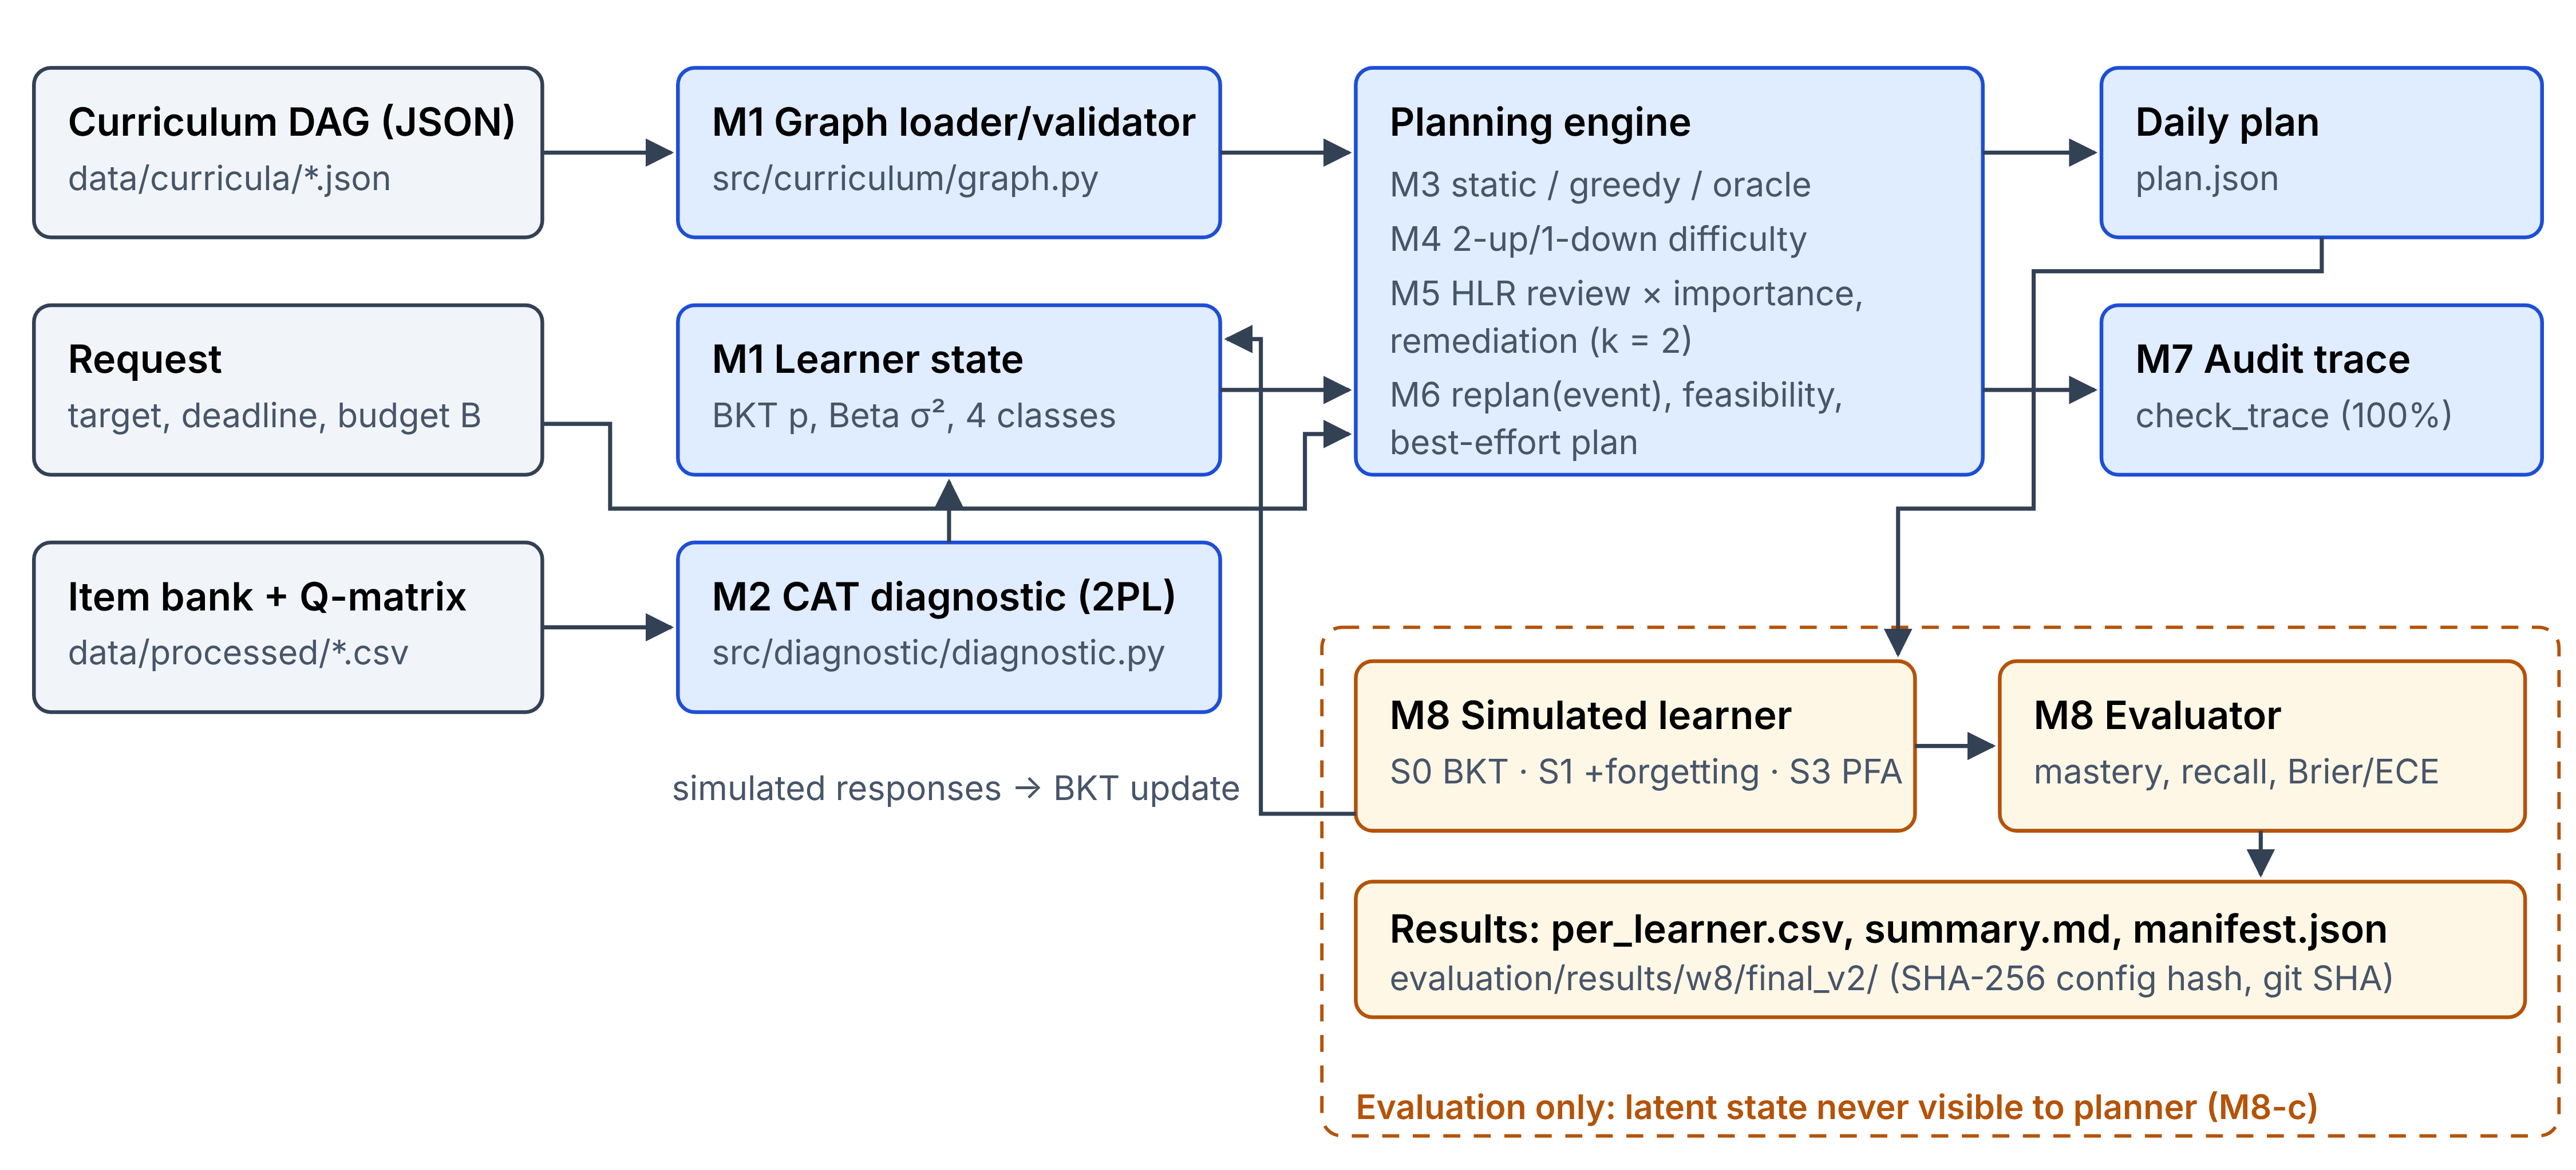
\includegraphics[width=\textwidth]{architecture.png}
    \caption{Components and data flow. Blue: engine modules. Amber: evaluation-only simulator and evaluator; their latent state is never visible to the planner (M8-c).}
    \label{fig:arch}
\end{figure}

\subsection{Major Components and Final Status}
{\small
\begin{longtable}{|C{1.11cm}|L{2.40cm}|L{5.82cm}|L{5.26cm}|}
\caption{Modules, interfaces and status at Week 8 (compare with Mid-Review Section C.2, status at Week 3).}\\
\hline
\textbf{Mod.} & \textbf{Component} & \textbf{Key functions / files} & \textbf{Status at Week 8} \\ \hline
\endfirsthead
\hline \textbf{Mod.} & \textbf{Component} & \textbf{Key functions / files} & \textbf{Status at Week 8} \\ \hline
\endhead
M1 & Graph loader and validator & \texttt{load\_graph}, \texttt{validate\_graph} $\cdot$ \rf{src/curriculum/graph.py} & Six checks incl.\ non-finite node and edge values (Mid-Review gap closed, W4 D5) \\ \hline
M1 & Learner-state model & \texttt{ConceptState.update}, \texttt{classify}, \texttt{PolicyConfig} $\cdot$ \rd{src/state} & BKT parity with pyBKT $<10^{-4}$; four classes; policy schema validated \\ \hline
M2 & Adaptive diagnostic & \texttt{run\_adaptive\_diagnostic}, \texttt{init\_from\_diagnostic} $\cdot$ \rf{src/diagnostic/diagnostic.py} & Live CAT implemented (W4); answers count as evidence (W8, B10) \\ \hline
M3 & Planners & \texttt{generate\_static\_plan}, \texttt{run\_greedy\_scheduler}, \texttt{run\_greedy\_best\_singleton}, \texttt{run\_exhaustive\_oracle} $\cdot$ \rd{src/planning} & Order-invariant oracle (W3); best-singleton fallback (W7) \\ \hline
M3/M6 & Feasibility and replanning & \texttt{check\_feasibility}, \texttt{replan(state, event)} $\cdot$ \rf{src/planning/replan.py} & Four events; practice-for-evidence (W7); best-effort plan (W8) \\ \hline
M4 & Difficulty policy & \texttt{step\_difficulty} $\cdot$ \rf{src/planning/difficulty.py} & 2-up/1-down implemented (W4) \\ \hline
M5 & Review and remediation & \texttt{rank\_due\_reviews}, \texttt{get\_remediation\_ancestors} $\cdot$ \rf{src/planning/review.py} & HLR review (W4), importance-weighted (W8, B11); remediation unit-tested \\ \hline
M7 & Audit trace & \texttt{TraceEntry}, \texttt{ReasonCode}, \texttt{check\_trace} $\cdot$ \rd{src/trace} & 11 reason codes; strict type and bound checks (W4 D4) \\ \hline
M8 & Simulation and evaluation & \texttt{MatchedBKTGenerator}, \texttt{MismatchedPFAOrLogisticGenerator}, \texttt{run\_integrated\_evaluation} $\cdot$ \rd{src/evaluation} & 9-arm harness, retention quiz, calibration, paired bootstrap \\ \hline
\end{longtable}
}

\subsection{Learner-State Model (M1)}
\label{sec:state}
\textbf{BKT update.} For a concept with mastery $p$, slip $s = 0.10$, guess $g = 0.25$ and learn rate $t = 0.10$,
\begin{equation*}
p_{\text{post}} =
\begin{cases}
\dfrac{p(1-s)}{p(1-s) + (1-p)g} & \text{if the answer is correct,}\\[2ex]
\dfrac{p\,s}{p\,s + (1-p)(1-g)} & \text{if it is incorrect,}
\end{cases}
\qquad
p \leftarrow p_{\text{post}} + (1-p_{\text{post}})\,t .
\end{equation*}
Each answer also increments the evidence count $n$ and the Beta concentration $\kappa$, and is appended to a window of the last $W=4$ answers.
\vspace{0.2em}\newline
\textbf{Uncertainty.} $\sigma^2 = p(1-p)/(\kappa+1)$. This counts evidence; it is a declared heuristic, not a calibrated credible interval (ADR-005). Calibration of $p$ is measured instead (Section~\ref{sec:calib}).

{\small
\begin{longtable}{|L{2.09cm}|L{6.47cm}|L{6.47cm}|}
\caption{Four-state classifier, evaluated in this precedence order (\rf{src/state/learner_state.py}).}\\
\hline
\textbf{State} & \textbf{Rule} & \textbf{Planner consequence} \\ \hline
\endfirsthead
\hline \textbf{State} & \textbf{Rule} & \textbf{Planner consequence} \\ \hline
\endhead
Uncertain & $n < 3$ or $\sigma^2 > 0.05$ & Never trusted: routed to assessment or practice-for-evidence (\path{UNCERTAIN_NEEDS_ASSESSMENT}) \\ \hline
Mastered & $p \geq 0.85$, $\sigma^2 \leq 0.05$, $n \geq 3$ and at least 3 of the last 4 answers correct & Unlocks dependents (\path{ALREADY_MASTERED}); eligible for review when recall decays \\ \hline
Weak & $p < 0.40$ with at least 3 of the last 4 answers incorrect & Blocks dependents; candidate for remediation \\ \hline
Developing & otherwise & Practised; dependents wait \\ \hline
\end{longtable}
}
\vspace{0.2em}\noindent
\textbf{Planned, completed and evidence-Mastered are three different states.} A concept placed on a future day is \textit{planned}; a dependent may be placed after it only \textit{conditionally} and is re-checked before it is done. \textit{Completed} means the learner did the activity. Only \textit{evidence-Mastered} unlocks dependents unconditionally; a failed prerequisite keeps its dependents blocked.
\vspace{0.2em}\newline
\textbf{Diagnostic priors (M2 $\rightarrow$ M1).} The CAT estimates ability $\hat\theta$ from up to 10 items chosen by maximum Fisher information from a 24-item 2PL bank, stopping early if $\mathrm{Var}(\hat\theta) \leq 0.15$. Concepts probed by the Q-matrix start with $p = \mathrm{sigmoid}(\hat\theta)$, and since Week 8 with $n = k$ answered items, $\kappa = 2 + k$ and those answers as history (ADR-009 amendment, \cm{70183b7}); unprobed concepts start cold (Beta(1,1), Uncertain).

\subsection{Planning and Adaptation Policies (M3--M6)}
\begin{itemize}
    \item \textbf{Frontier.} A concept is a candidate on day $d$ if it is the target or an ancestor, is not evidence-Mastered or already scheduled, and its prerequisites are Mastered or planned earlier (conditional). Every candidate gets exactly one trace entry per day.
    \item \textbf{Greedy selection.} Candidates are ranked by score per minute with deterministic tie-breaking and packed while they fit the remaining budget. The \textbf{best-singleton fallback} (W7) also evaluates the best single item that fits and keeps whichever scores higher, the classic fix for knapsack counterexamples. The \textbf{exact oracle} enumerates precedence-closed subsets ($N \leq 20$, with a timeout) and is used to measure greedy quality.
    \item \textbf{Feasibility.} \path{INFEASIBLE_PROVED} is returned only for proved cases: a block longer than $B$ (fix: raise the budget to the longest block; more days cannot help) or required work $W_{\text{req}} > D \times B$ (fixes: the minimum budget or number of days). \path{FEASIBLE} requires a witness plan; if packing fails without a proof the status is \path{HEURISTIC_NO_PLAN}. Since Week 8 a proved-infeasible request also returns a \textbf{best-effort plan} of the work that fits instead of idling.
    \item \textbf{Difficulty (M4).} Difficulty $d \in [0.05, 0.95]$: one incorrect answer lowers $d$ by 0.10; two consecutive correct answers raise it by 0.10; an Uncertain concept returns to its curriculum baseline.
    \item \textbf{Spaced review (M5).} Predicted recall $R = 2^{-\Delta t/14}$. A Mastered concept is due when $R < 0.85$. Due reviews use only leftover minutes and are packed by priority $(1-R)\times w$, where $w$ is the largest edge importance from the concept to a not-yet-Mastered dependent (default 1.0) (\cm{edde468}). Recall, weight and priority are written to the trace (\path{REVIEW_DUE}).
    \item \textbf{Remediation (M5).} Two consecutive failed assessments on a concept insert its lowest-mastery unmet prerequisite (\path{REMEDIATION_TRIGGERED}); forward progress on that branch pauses until the prerequisite is evidence-Mastered.
    \item \textbf{Replanning (M6).} \texttt{replan(state, event)} handles \texttt{assessment\_result}, \texttt{missed\_day}, \texttt{changed\_budget} and \texttt{changed\_deadline}. Completed work is kept and only the future is recomputed. A completed prerequisite that is still Uncertain or Weak and blocks remaining work receives one practice block (\path{PRACTICE_FOR_EVIDENCE}, Week 7 deadlock fix, \cm{c5d1a8f}).
\end{itemize}

\subsection{Interactions and Workflow}
\begin{figure}[H]
    \centering
    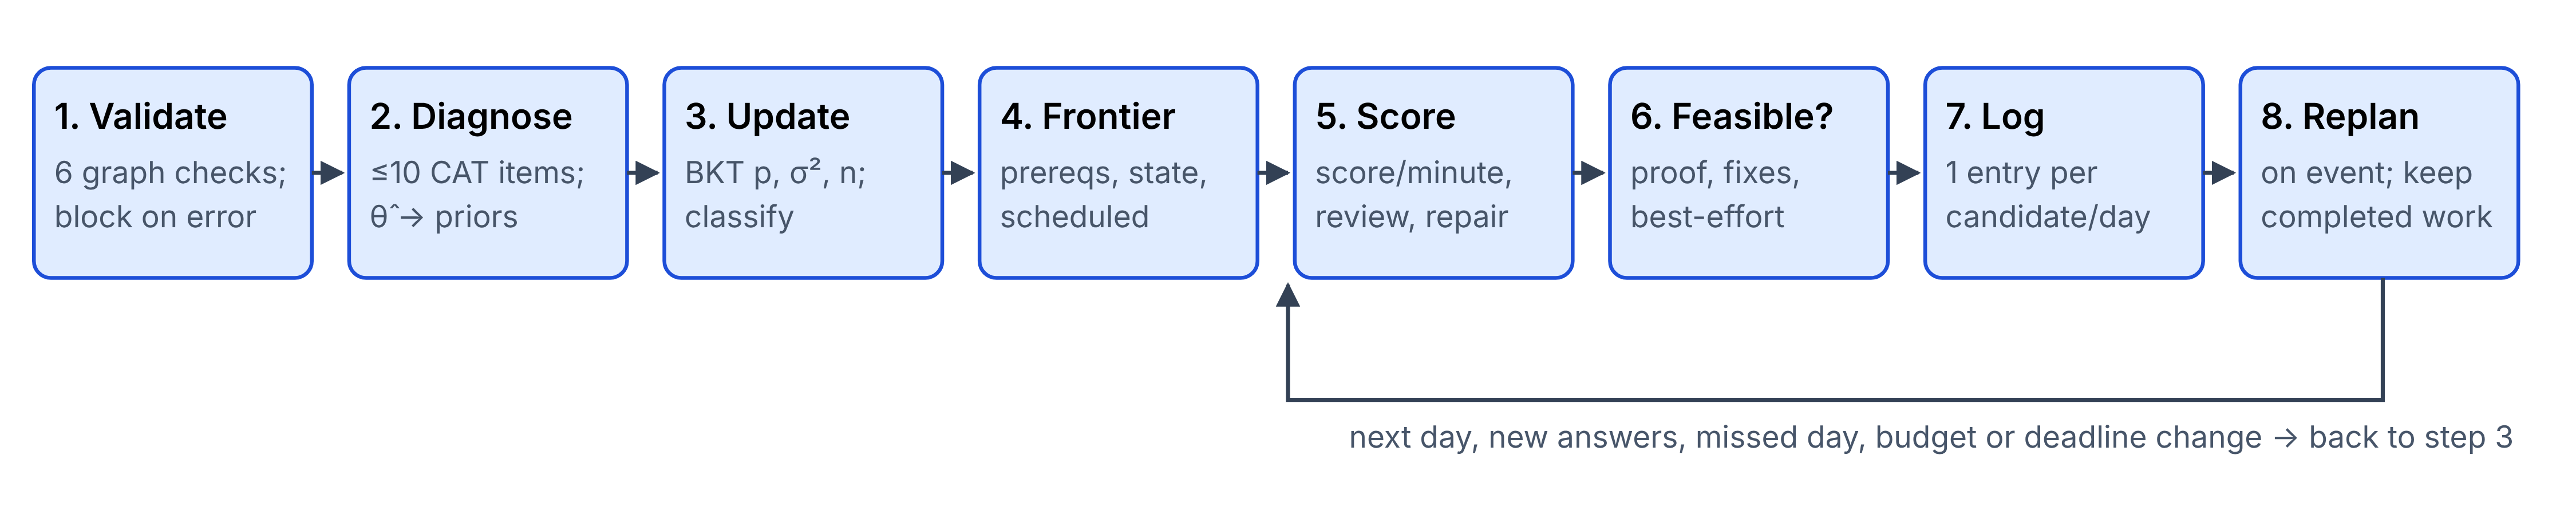
\includegraphics[width=\textwidth]{images/workflow.png}
    \caption{Daily workflow. Steps 3--8 repeat every day and after every event.}
\end{figure}
\begin{enumerate}
    \item \textbf{Validate.} Any graph error blocks planning and returns a structured error instead of a fallback plan.
    \item \textbf{Diagnose.} A new learner takes the bounded CAT; $\hat\theta$ sets the priors of probed concepts.
    \item \textbf{Update.} Every scored answer updates $p$, $\sigma^2$, $n$ and the class.
    \item \textbf{Build the frontier} from prerequisites, states and earlier days.
    \item \textbf{Score and select.} Candidates are scored; review and remediation compete for the same day's minutes.
    \item \textbf{Check feasibility.} A witness plan, a proof with fixes, or a best-effort plan is returned.
    \item \textbf{Log.} The trace records one disposition per candidate per day with the state and constraints at decision time.
    \item \textbf{Observe and replan} on an assessment result, a missed day, or a changed budget or deadline.
\end{enumerate}

\subsection{Inputs, Outputs and the Audit Trace}
\textbf{Inputs:} Curriculum JSON: nodes (\texttt{node\_id}, \texttt{concept\_name}, \texttt{baseline\_duration}, \texttt{exercises}, \texttt{base\_difficulty}) and edges (\texttt{source}, \texttt{target}, \texttt{importance}); learner responses (concept, correct, timestamp); constraints ($B$, $D$, target); and one policy configuration per run (BKT parameters, window, thresholds, seeds), hashed with SHA-256.
\vspace{0.2em}\newline
\textbf{Outputs:} \texttt{plan.json} (per day: activities, conditional activities, minutes used and left; the feasibility explanation; assessment candidates), concept states, the next difficulty, a feasibility verdict and the trace. Each trace entry has eight fields: \texttt{day}, \texttt{node\_id}, \texttt{decision}, \texttt{reason\_code}, \texttt{concept\_state} ($p$, $\sigma^2$, $n$, $\kappa$, class), \texttt{constraints} (budget, remaining budget, prerequisites, conditional), \texttt{score\_terms} and \texttt{policy\_version}. A sample is in Appendix~\ref{app:sample}.

{\small
\begin{longtable}{|L{3.97cm}|L{3.32cm}|L{3.97cm}|L{3.32cm}|}
\caption{Reason codes (\rf{src/trace/schema.py}). The Mid-Review had eight; three were added for review, remediation and practice-for-evidence.}\\
\hline
\textbf{Code} & \textbf{Meaning} & \textbf{Code} & \textbf{Meaning} \\ \hline
\endfirsthead
\hline \textbf{Code} & \textbf{Meaning} & \textbf{Code} & \textbf{Meaning} \\ \hline
\endhead
\path{SELECTED} & Scheduled today & \path{BLOCK_EXCEEDS_DAILY_BUDGET} & Activity longer than $B$ (proved infeasible) \\ \hline
\path{PREREQUISITE_UNMET} & A prerequisite is not Mastered or planned & \path{BUDGET_EXCEEDED} & Does not fit today's remaining minutes \\ \hline
\path{ALREADY_MASTERED} & Evidence-Mastered; no new learning needed & \path{UNCERTAIN_NEEDS_ASSESSMENT} & Not enough evidence; route to assessment \\ \hline
\path{ALREADY_SCHEDULED} & Planned on an earlier day & \path{REVIEW_DUE} & Mastered but predicted recall $<0.85$ \\ \hline
\path{COMPLETED} & Already done by the learner & \path{REMEDIATION_TRIGGERED} & Prerequisite inserted after two failures \\ \hline
\path{PRACTICE_FOR_EVIDENCE} & Completed but unproven prerequisite gets practice (W7) & & \\ \hline
\end{longtable}
}

\subsection{User Interface: Project Website and Live Demos}
\label{sec:ui}
\textbf{Purpose.} The brief asks the system to ``expose why a lesson was chosen''. The website lets a mentor or reviewer see the engine plan, replan and explain itself without installing anything, and browse every reported result. It is a demonstration interface, not a learner-facing product (an LMS is out of scope).
\vspace{0.2em}\newline
\textbf{How it works.} A static site in \rd{site}, published with GitHub Pages at \href{\siteurl}{\nolinkurl{bhuvan-56.github.io/adaptive-learning-path-planner-DAT/site/}}. The live demos run the project's own Python modules from \texttt{src/} in the browser through Pyodide 0.26.4; \rf{site/py/demo_api.py} only converts JSON in and out, so nothing is re-implemented in JavaScript. If Pyodide cannot be downloaded (about 10\,MB, once), the page says so and shows the saved outputs of every preset from \rf{site/data/fallback.json}, which \rf{site/build_data.py} produces by running the same code natively. The results pages read JSON that the same script recomputes from the per-learner CSVs; it refuses to write unless every number equals the committed result files.

{\small
\begin{longtable}{|L{3.04cm}|L{9.80cm}|L{2.19cm}|}
\caption{Website pages and what each demonstrates.}\\
\hline
\textbf{Page} & \textbf{What the user can do} & \textbf{Milestones} \\ \hline
\endfirsthead
\hline \textbf{Page} & \textbf{What the user can do} & \textbf{Milestones} \\ \hline
\endhead
Overview & Engine summary (Diagnostic $\rightarrow$ Learner state $\rightarrow$ Daily plan $\rightarrow$ Replan), headline numbers with sources, Week 7--8 changes & All \\ \hline
Curriculum & Switch between the 16-concept maths and 4-concept toy curricula; inspect durations, difficulty, exercises and prerequisite importance; click a concept to highlight its prerequisites & M1 \\ \hline
Live demo A: greedy vs oracle & Edit items (minutes, score, prerequisites) and a budget; run greedy, greedy + best-singleton and the exact oracle; presets reproduce the 12/18 counterexample and benchmark instance 215 & M3 \\ \hline
Live demo B: plan builder & Choose curriculum, target, budget and deadline; type each concept's answers (e.g.\ 1111, 0000, 1010); see learner states, the day-by-day plan drawn on the graph and the full trace with reason codes; apply one replan event & M1, M3--M7 \\ \hline
Scheduling benchmark & Ratio distribution over 250 instances, paired difference, changed instances, saved bad cases & M3, M8 \\ \hline
Results & S0/S1 arm tables with CIs, paired differences, the Week 8 before/after, the $2\times2$ robustness table & M8 \\ \hline
Simulation (20 Nov) & Play recorded sessions step by step: the S0 simulated learner answers the CAT diagnostic and daily practice towards Integrals (33--36 steps); engine estimate beside evaluator-only truth, mastery chart, plan, trace and change log. With the local server, simulate new learners & M1--M8 \\ \hline
Live session (20 Nov) & A person answers hand-written questions; wrong options name the mistake; the engine diagnoses, plans and replans after each answer; undo and ``skip 4 days'' & M1--M7 \\ \hline
\end{longtable}
}

\begin{figure}[H]
    \centering
    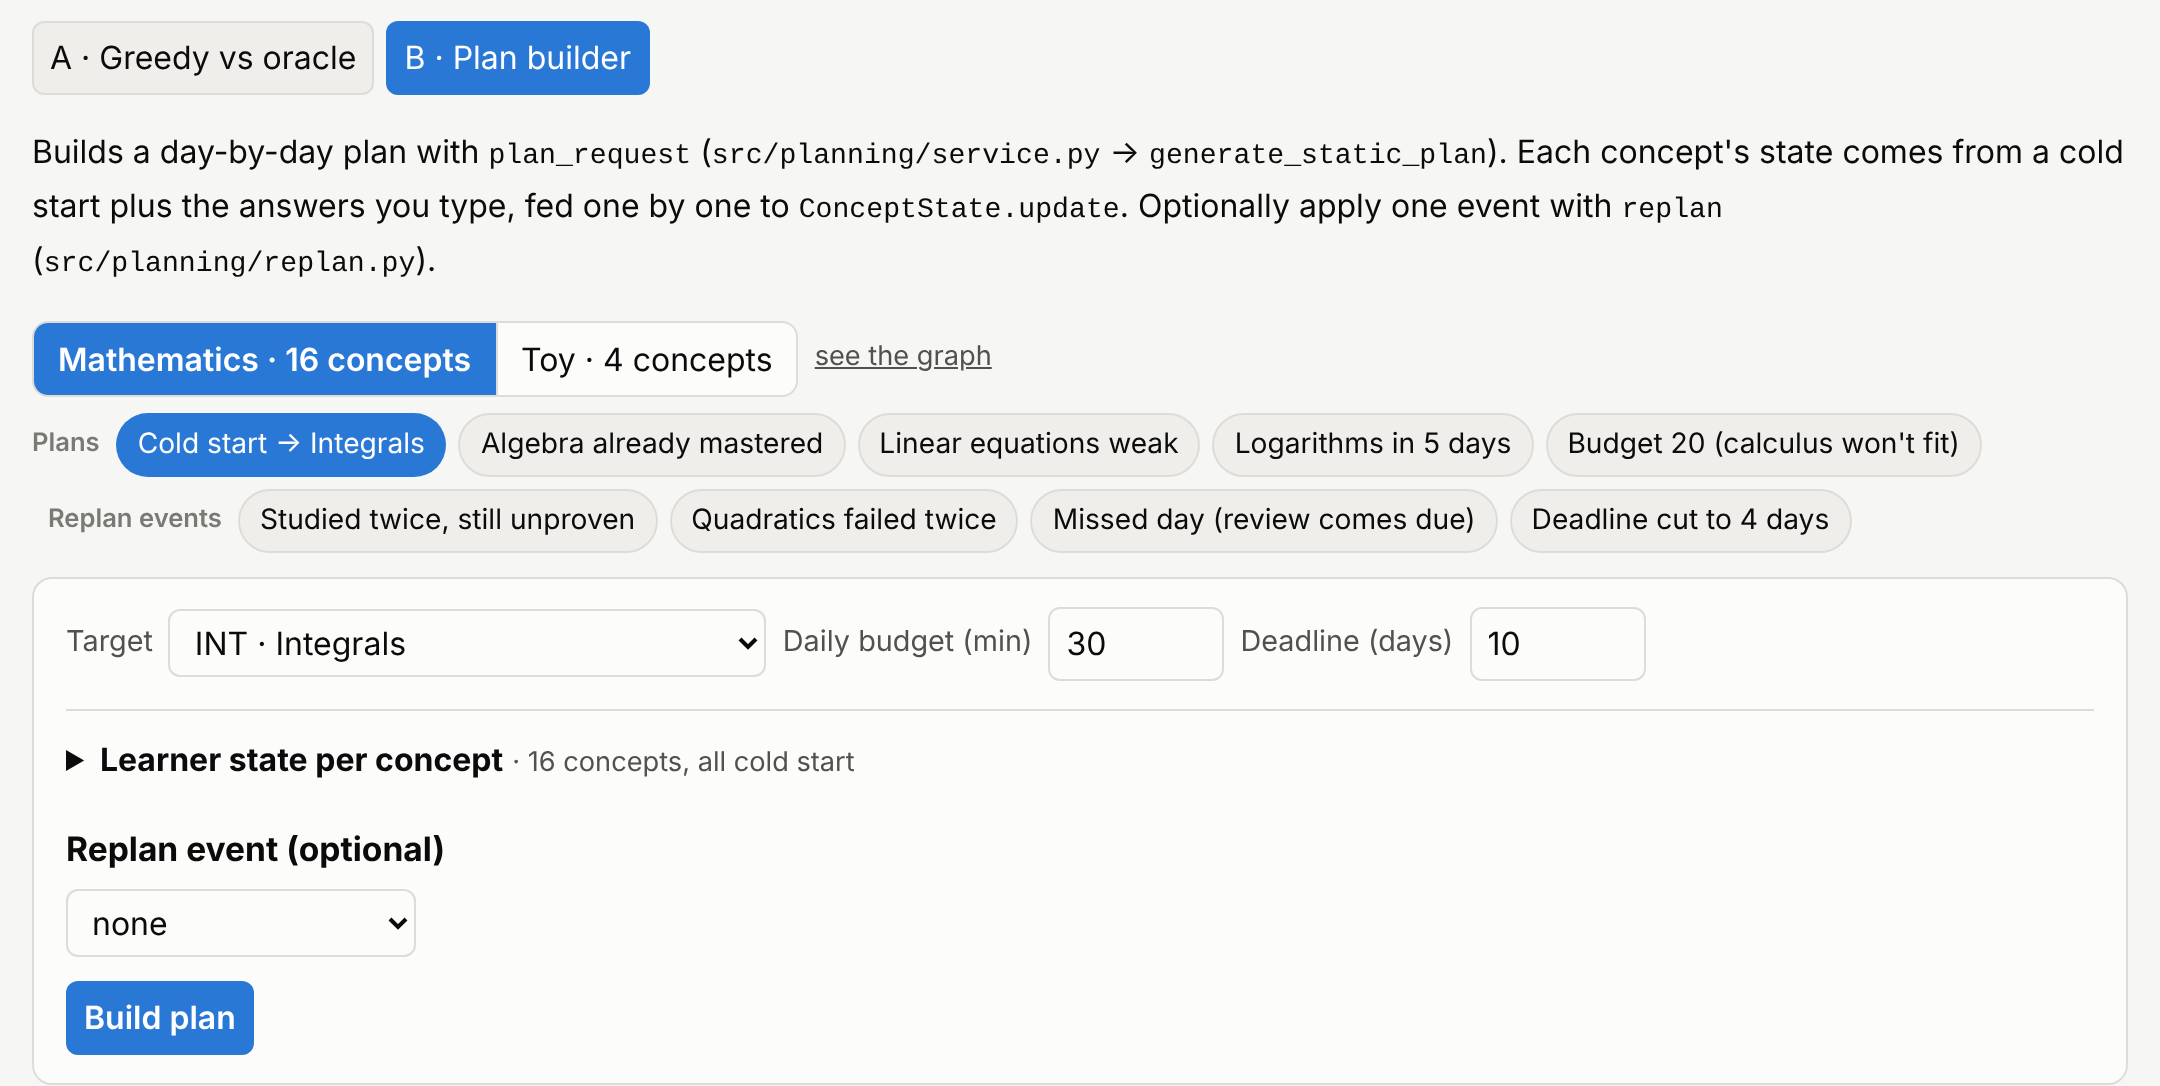
\includegraphics[width=0.9\textwidth]{images/ui_demoB_form.png}
    \caption{Demo B inputs: curriculum switch, plan presets (``Cold start $\rightarrow$ Integrals'', ``Algebra already mastered'', ``Budget 20 (calculus won't fit)'') and replan events, target, budget and deadline, per-concept answers and an optional event.}
\end{figure}

\begin{figure}[H]
    \centering
    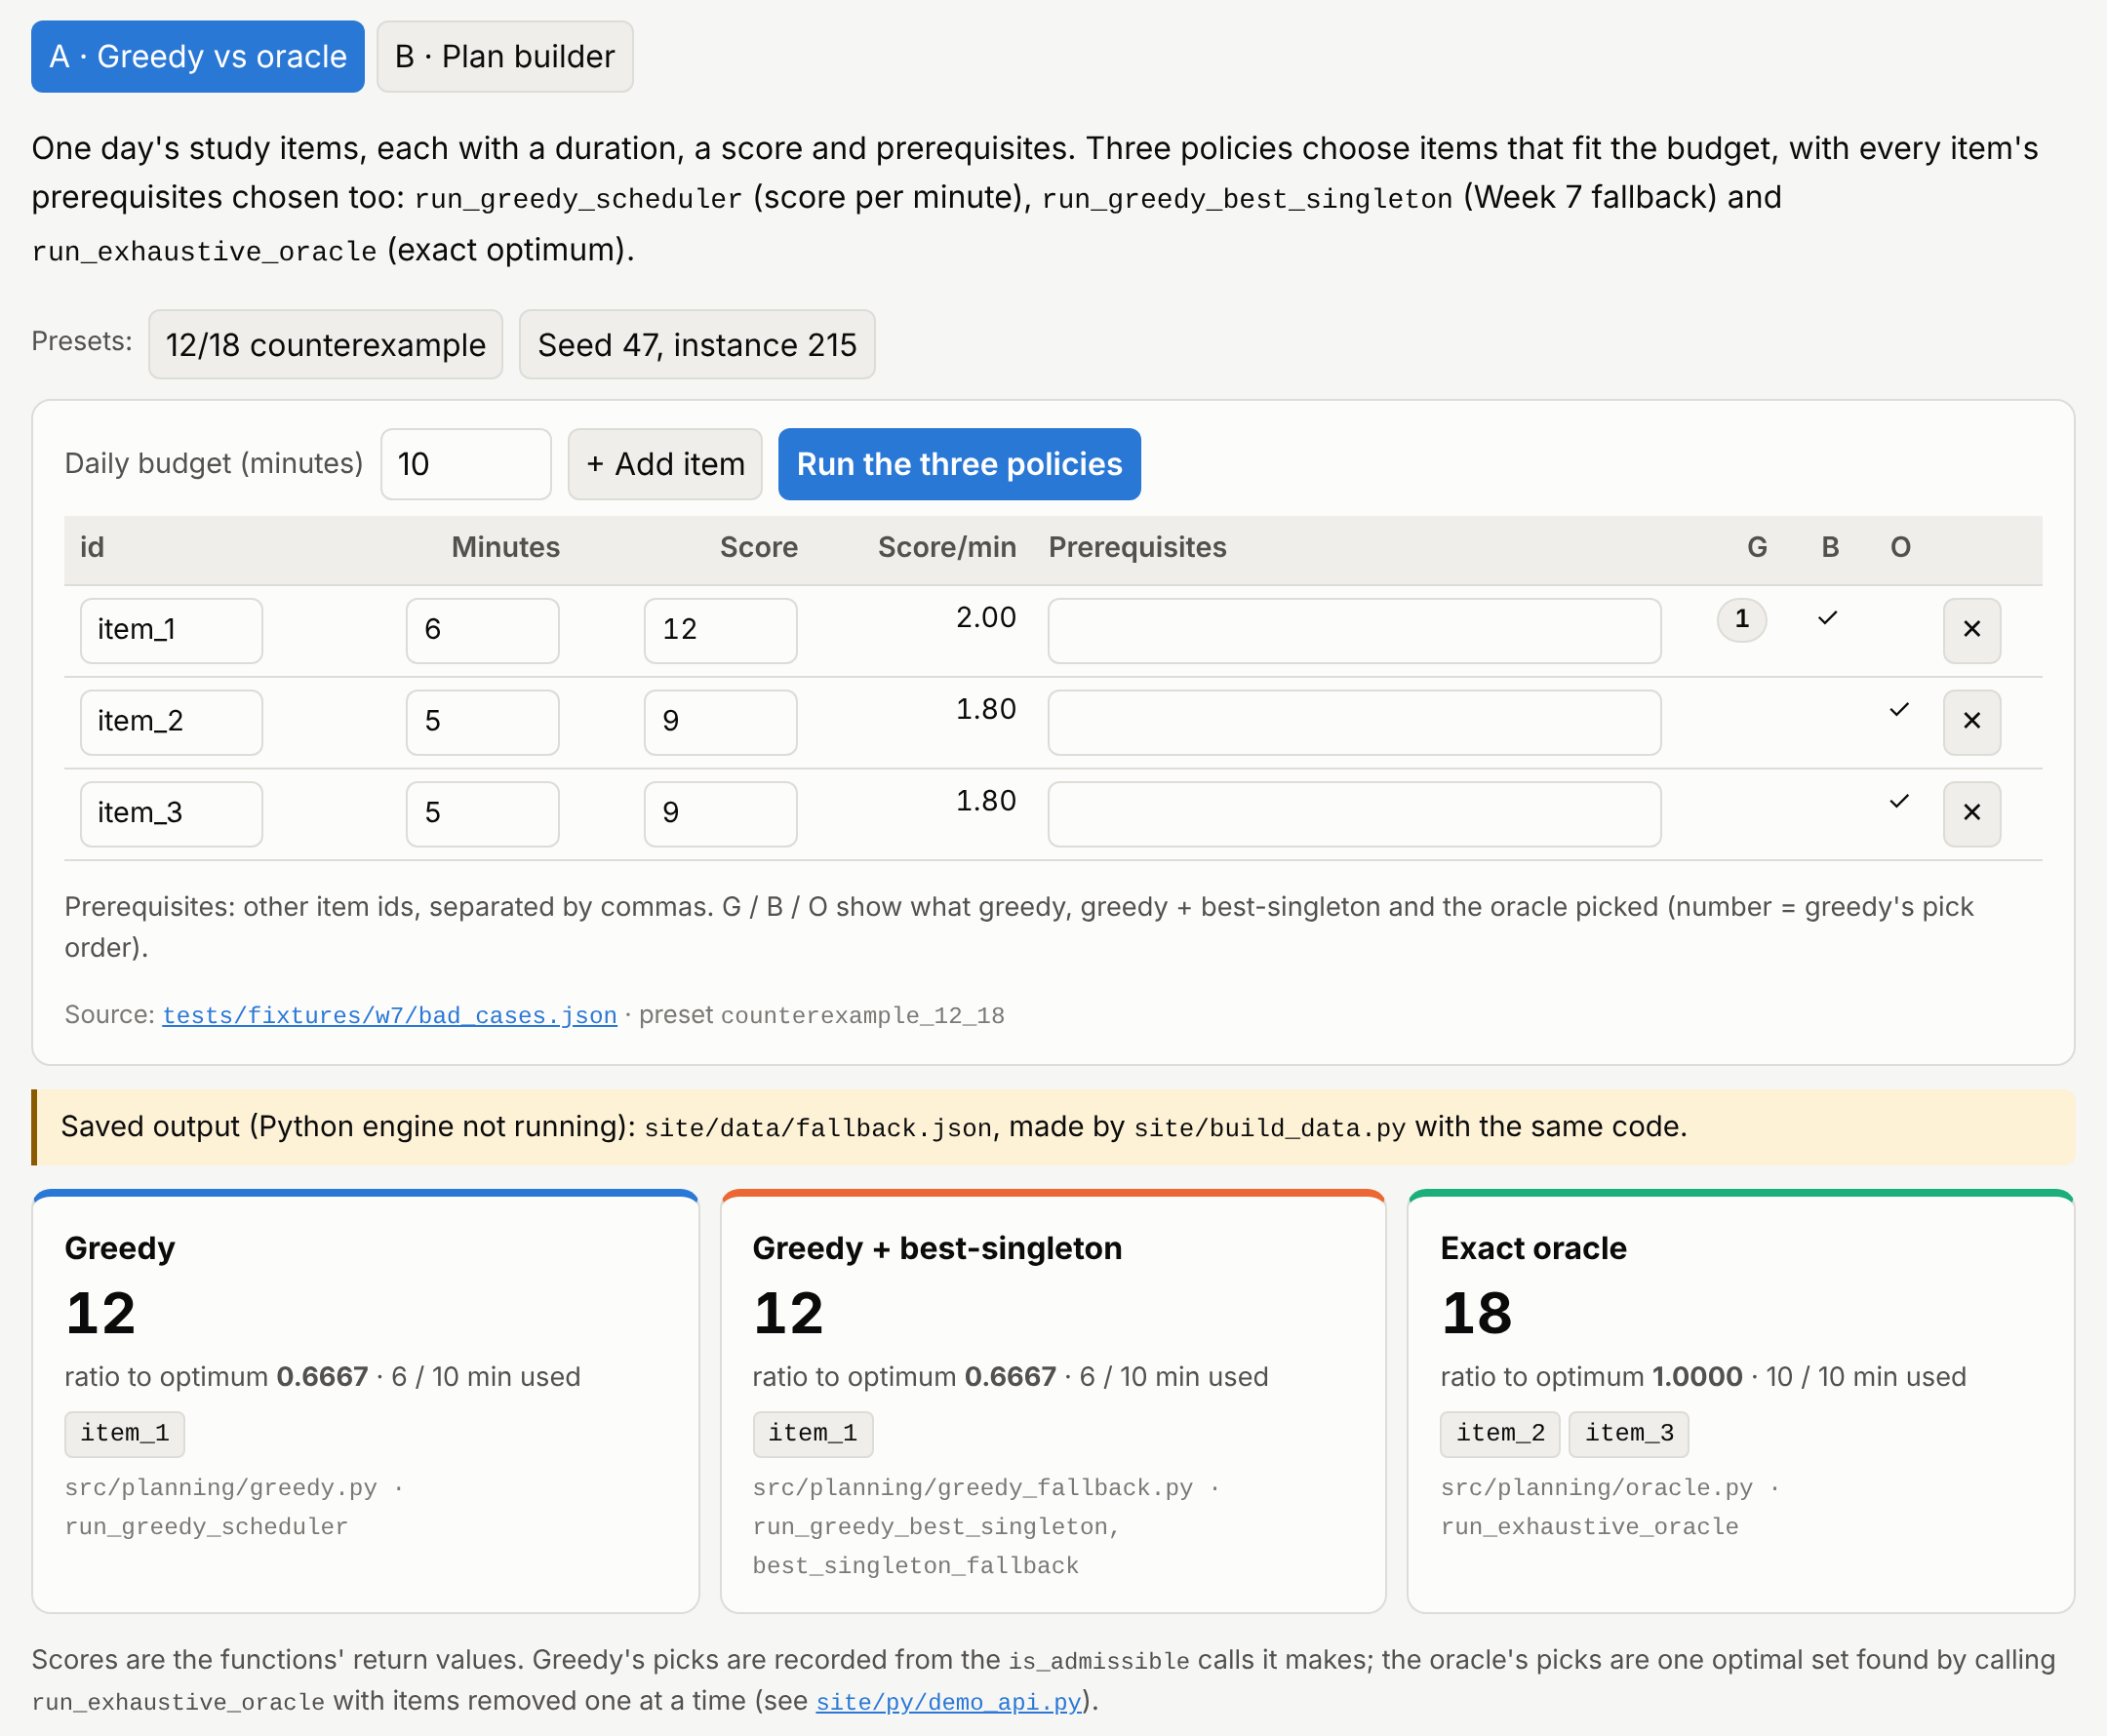
\includegraphics[width=0.65\textwidth]{images/ui_demoA.png}
    \caption{Demo A, preset ``12/18 counterexample'': greedy and greedy + best-singleton both score 12 (ratio 0.667); the exact oracle finds 18.}
\end{figure}

\begin{figure}[H]
    \centering
    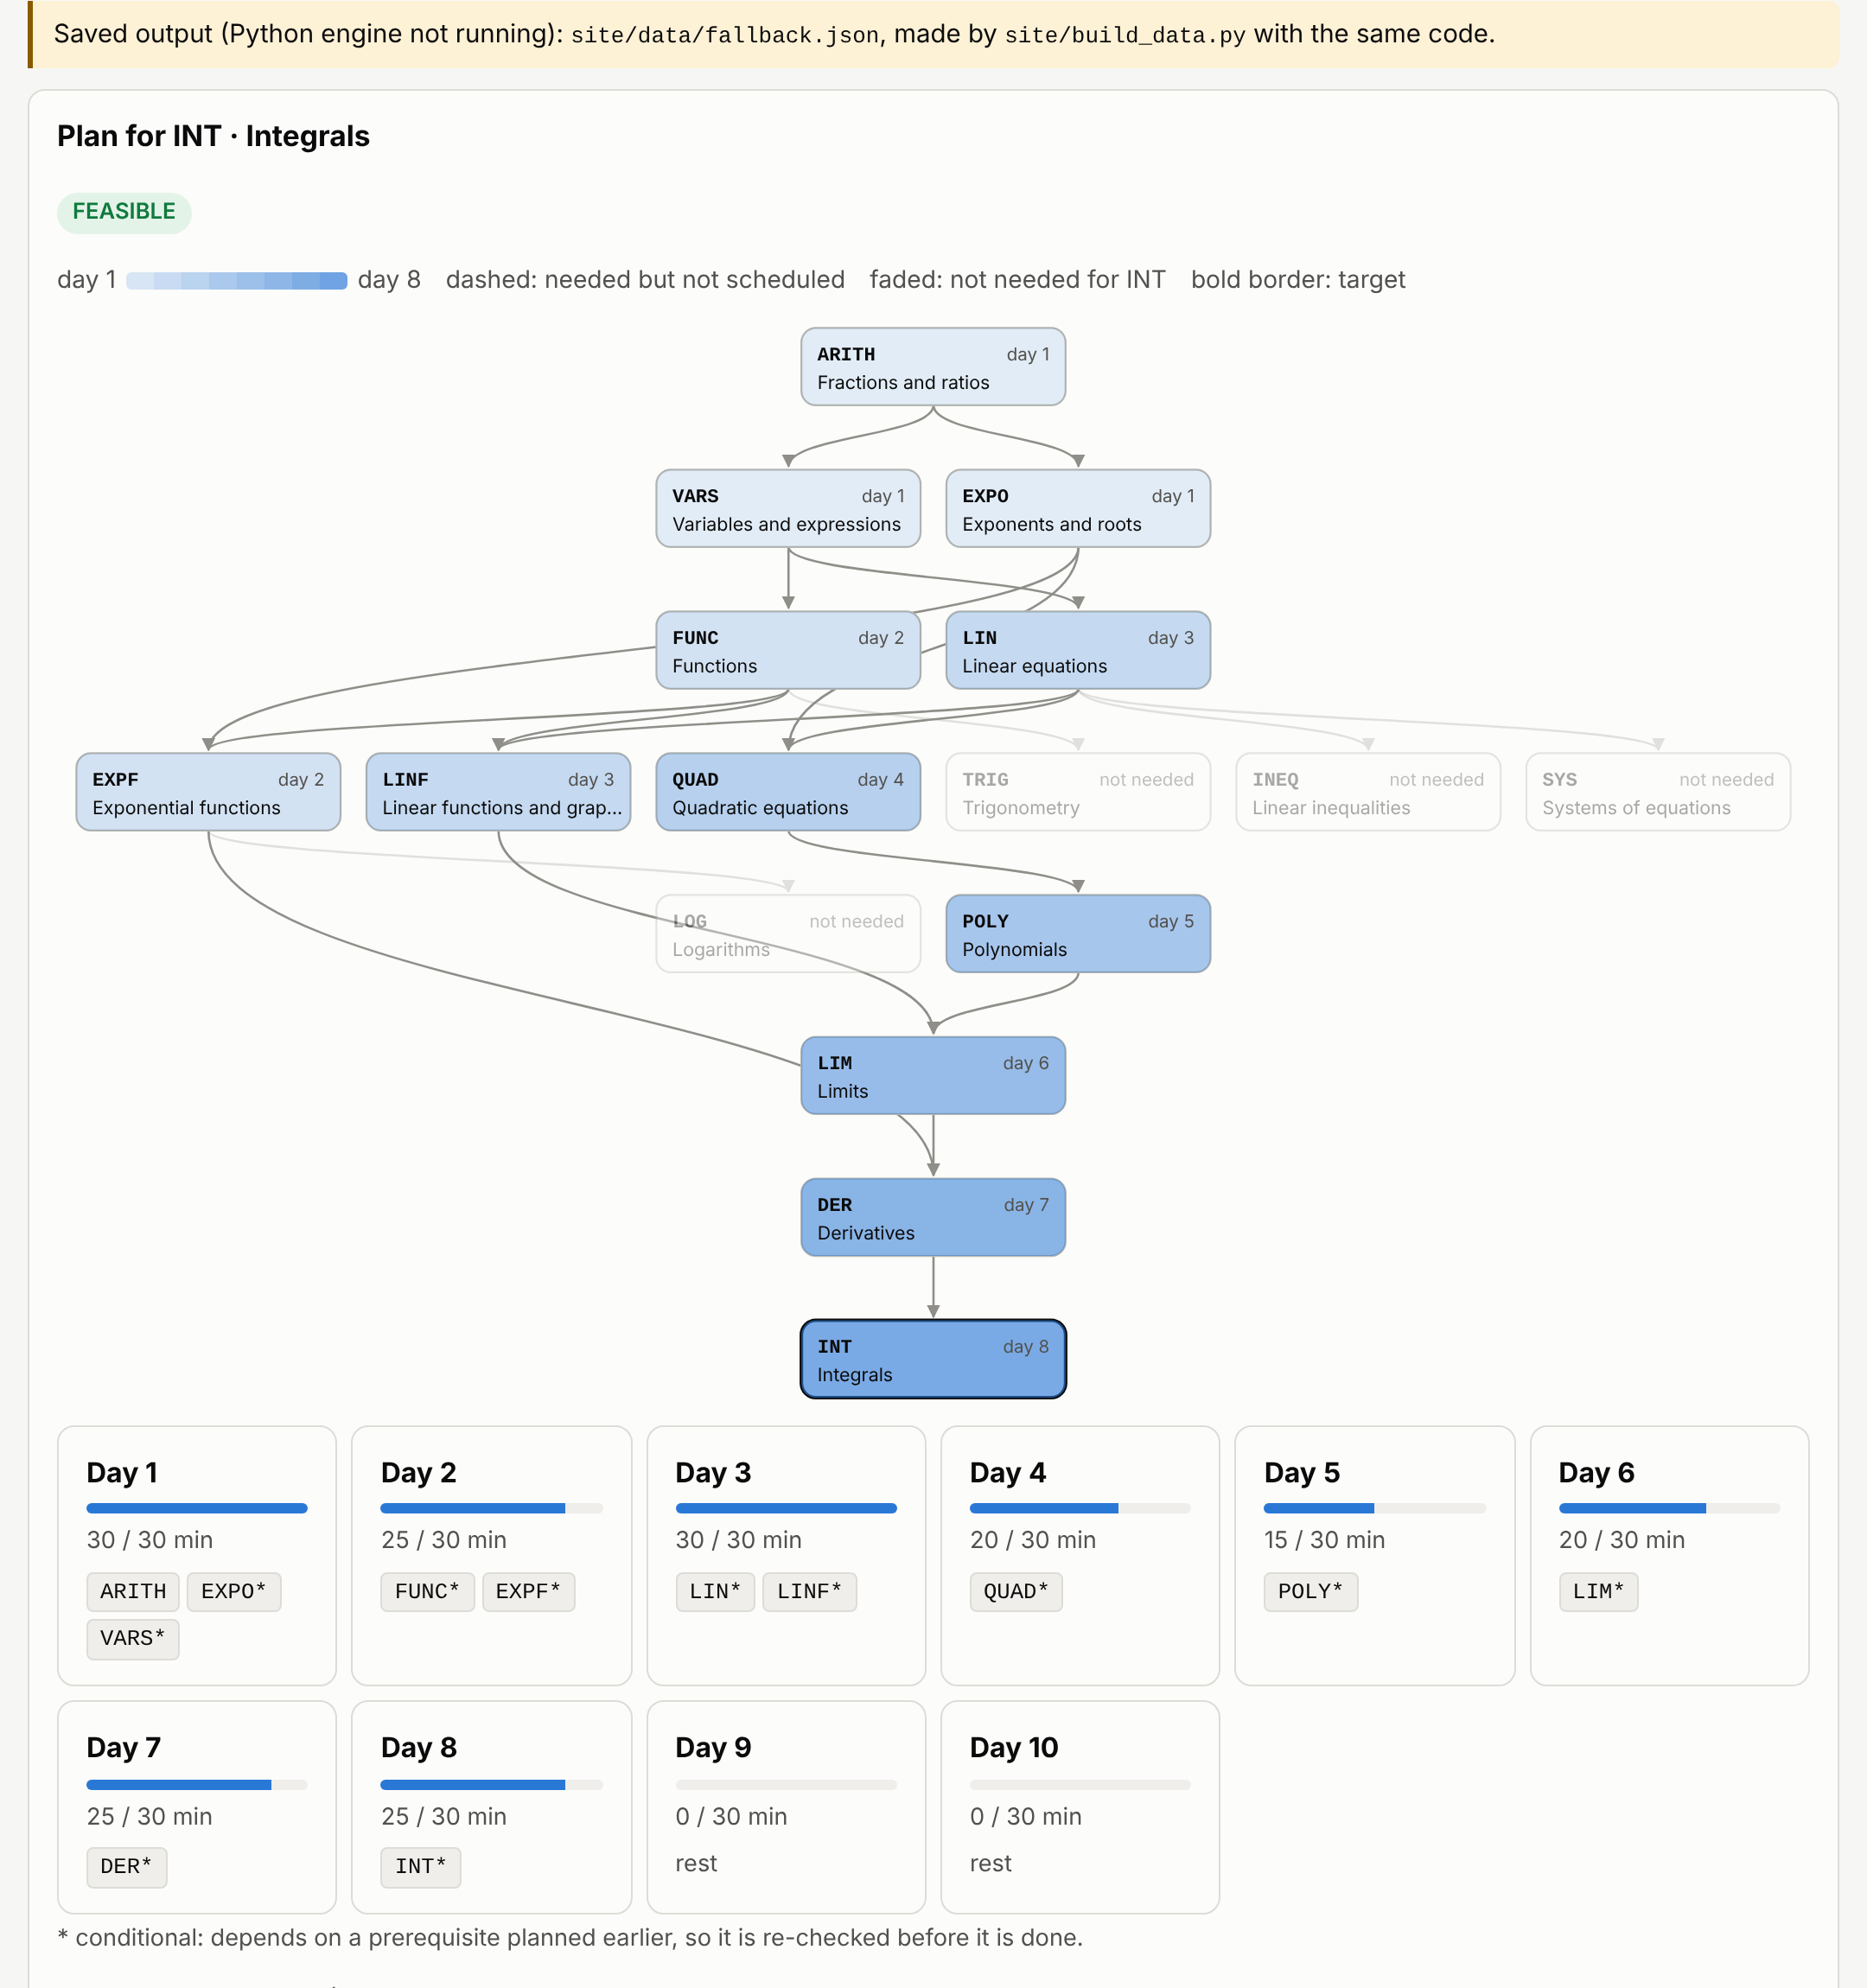
\includegraphics[width=0.70\textwidth]{images/ui_demoB_plan.png}
    \caption{Demo B on the maths curriculum, cold start, target Integrals, 30 min/day for 10 days: status FEASIBLE; the planned day of each concept is drawn on the prerequisite graph (concepts not needed for Integrals are faded) and summarised per day below (minutes used / budget).}
\end{figure}

\begin{figure}[H]
    \centering
    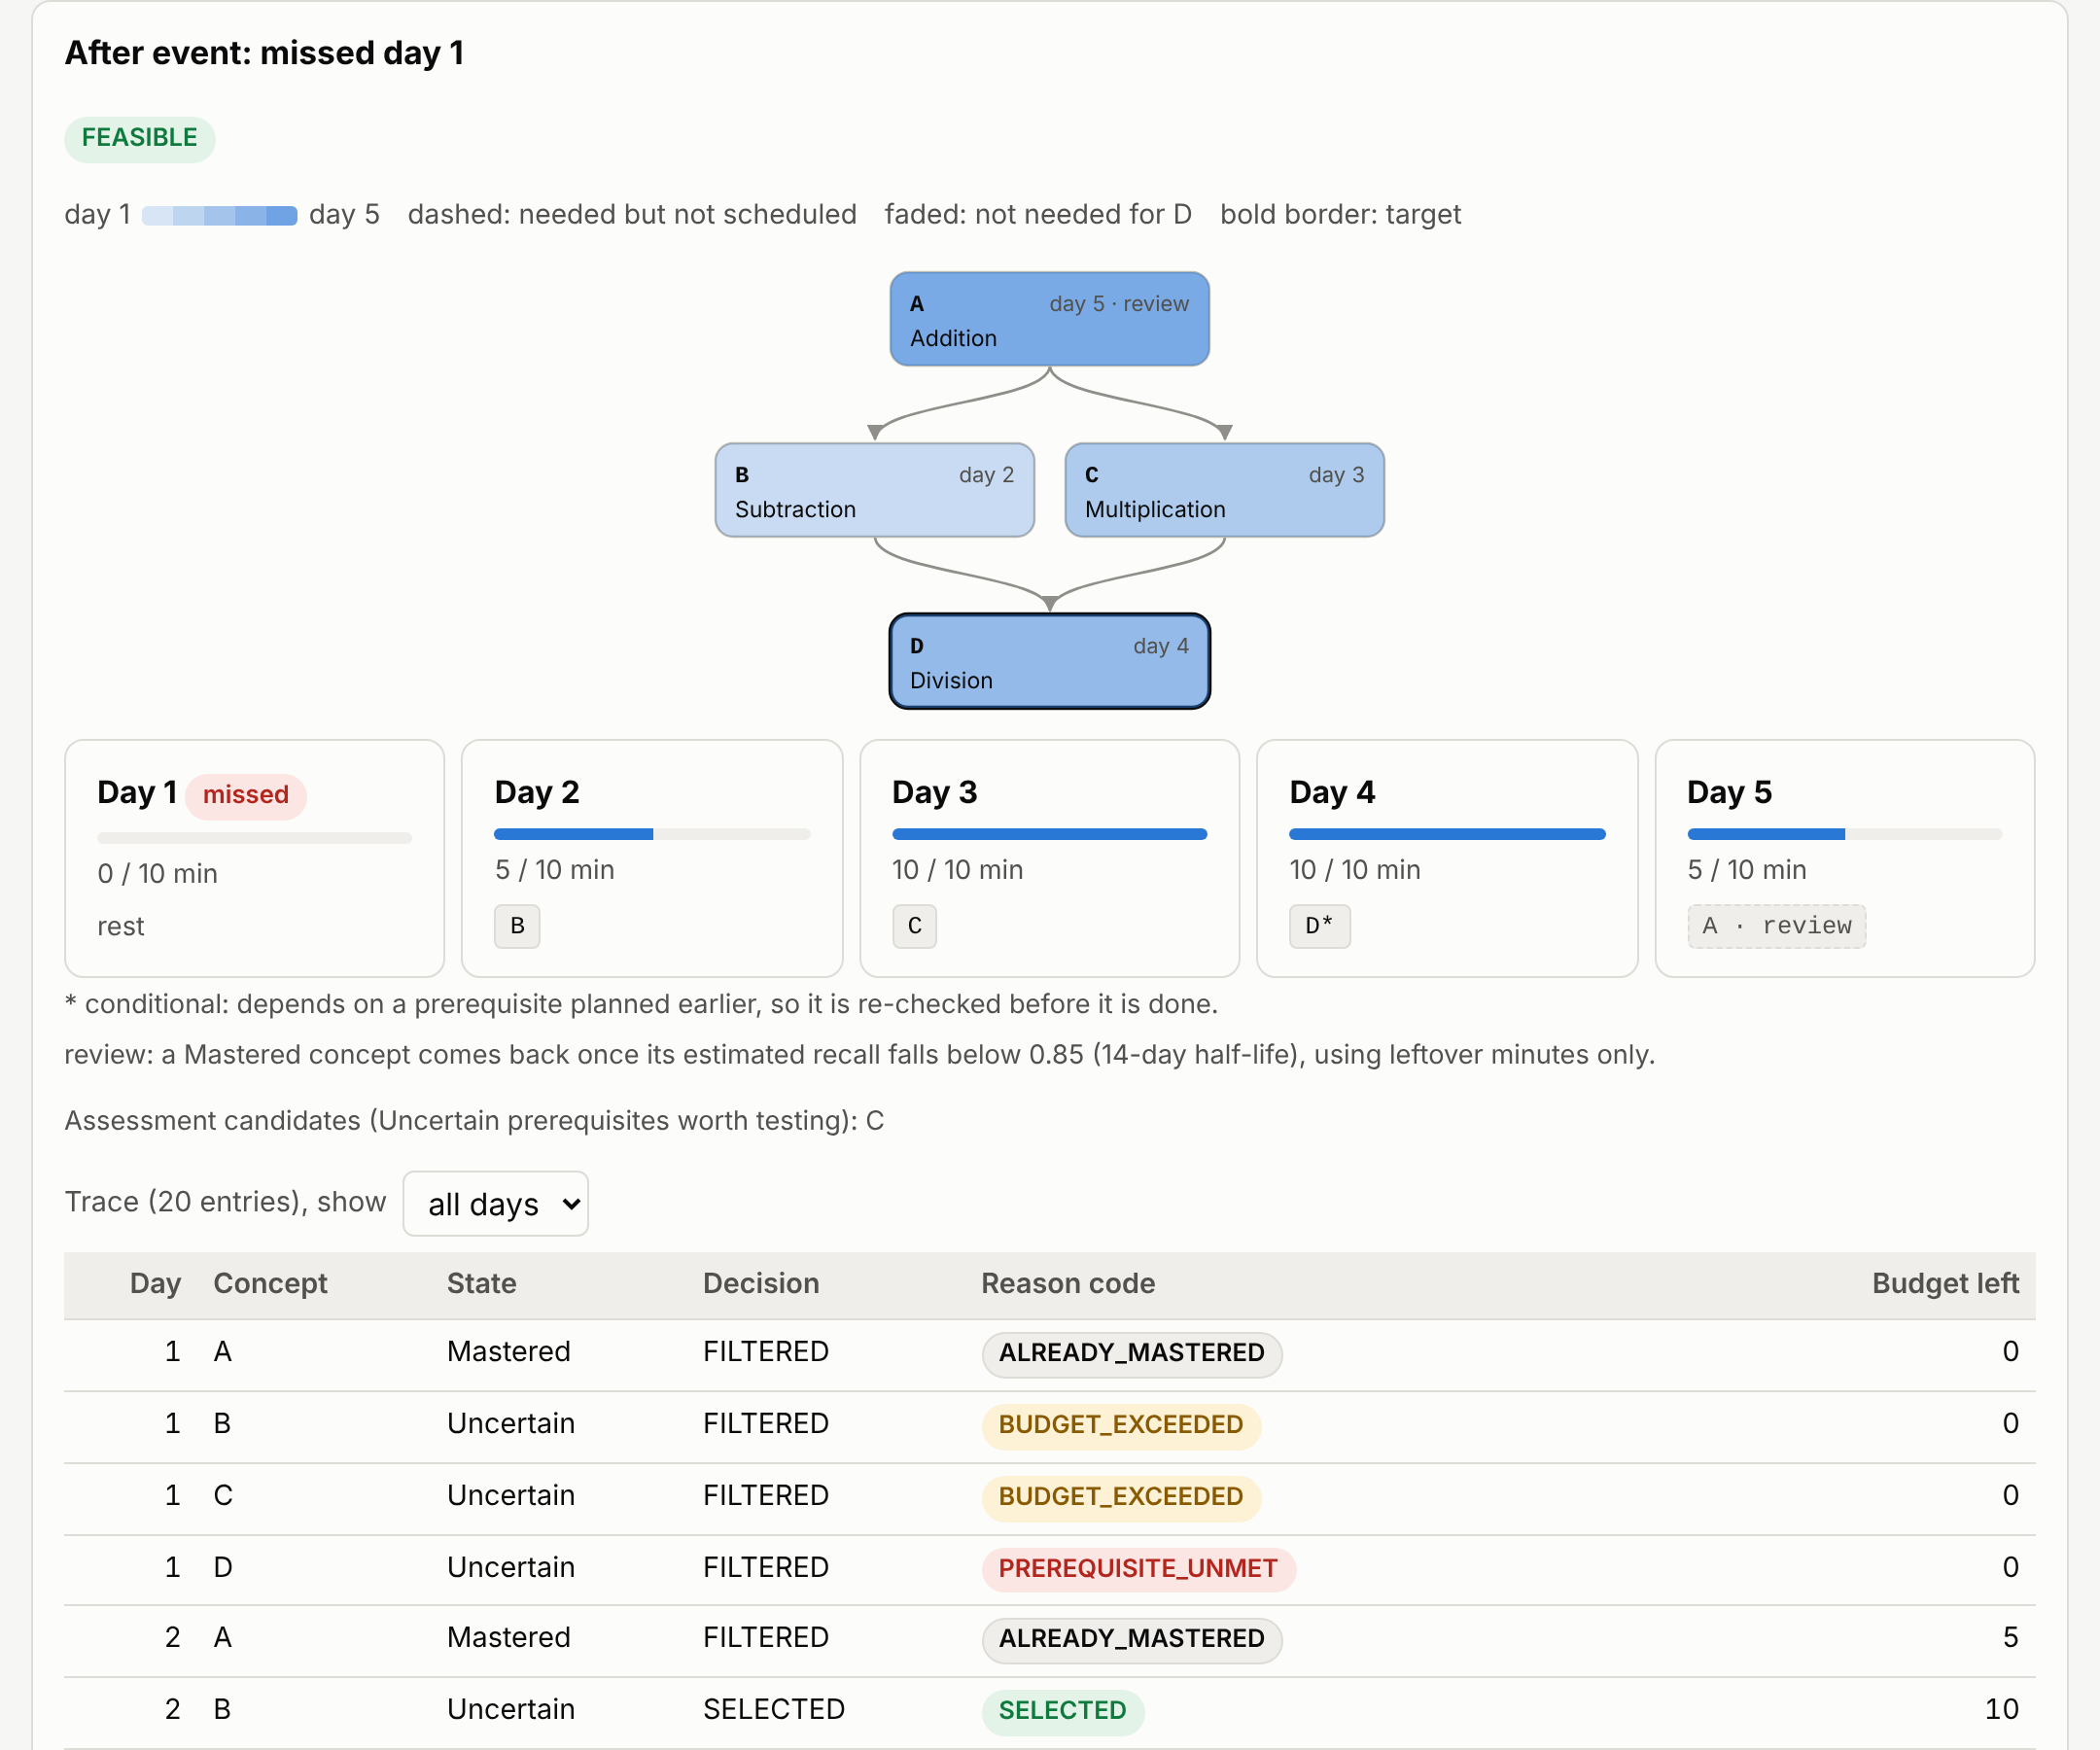
\includegraphics[width=0.80\textwidth]{images/ui_demoB_replan.png}
    \caption{Demo B replan, toy curriculum, event ``missed day 1'': completed work is kept, the plan shifts by a day, and a review of Addition appears on day 5 in leftover minutes. The trace table lists every candidate with its reason code and remaining budget.}
\end{figure}

\begin{figure}[H]
    \centering
    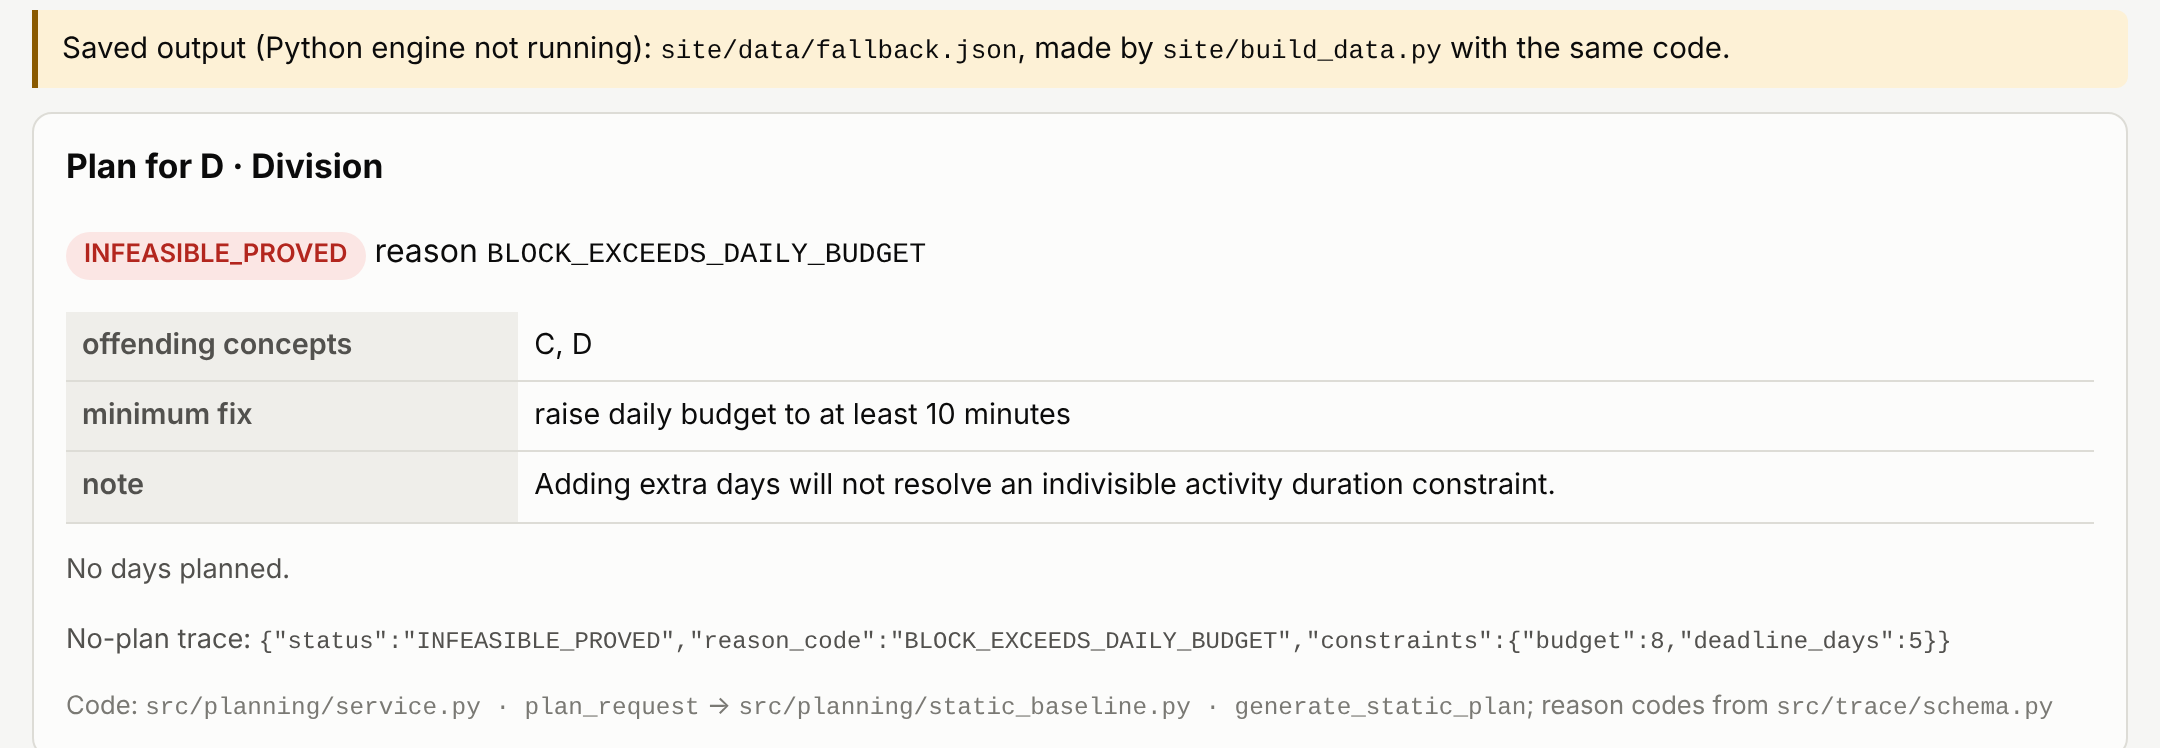
\includegraphics[width=0.86\textwidth]{images/ui_demoB_infeasible.png}
    \caption{Demo B, ``Budget 8 (infeasible)'': \texttt{INFEASIBLE\_PROVED} with reason \texttt{BLOCK\_EXCEEDS\_DAILY\_BUDGET}, the offending concepts, the minimum fix (raise the budget to 10) and the note that extra days cannot help.}
\end{figure}
\vspace{0.2em}\noindent
\textbf{Mapping to milestones.} Demo B shows M1 (states computed from typed answers), M3 (a time-budgeted, prerequisite-valid plan), M6 (replanning and infeasibility), M5 (reviews in leftover minutes) and M7 (the trace behind every decision). Demo A shows the M3 limitation that motivated the Week 7 fallback. The Results and Scheduling pages are the M8 evidence. More screenshots are in Appendix~\ref{app:ui}.
\vspace{0.2em}\newline
\textbf{Simulation and live session (Week 8 extension).} These pages run the full adaptive loop, including the CAT diagnostic. The diagnostic needs catsim and SciPy, which are too large for a reliable Pyodide download (in testing, the first 241\,KB of Pyodide took about 58\,s). So \rfx{site/serve_live.py}, a standard-library server bound to 127.0.0.1, runs \rfx{site/py/live_session.py} in the project's own Python. That module replays the \texttt{adaptive\_full} loop of the evaluation harness (first plan, \texttt{step\_difficulty}, \texttt{replan} after every answer) with a person or the S0 simulated learner answering, and changes no engine code. The Simulation page also plays runs recorded from that engine (\rfx{site/data/live_sim.json}), so it works on GitHub Pages. Questions are hand-written for the demo (\rfx{data/demo/questions_maths.json}): the 24 diagnostic items match the maths item bank, and every curriculum concept has practice questions. \rfx{tests/test_w8_live_demo.py} checks replay determinism, the diagnostic hand-over, the daily budget and skipped days.
\begin{figure}[H]
    \centering
    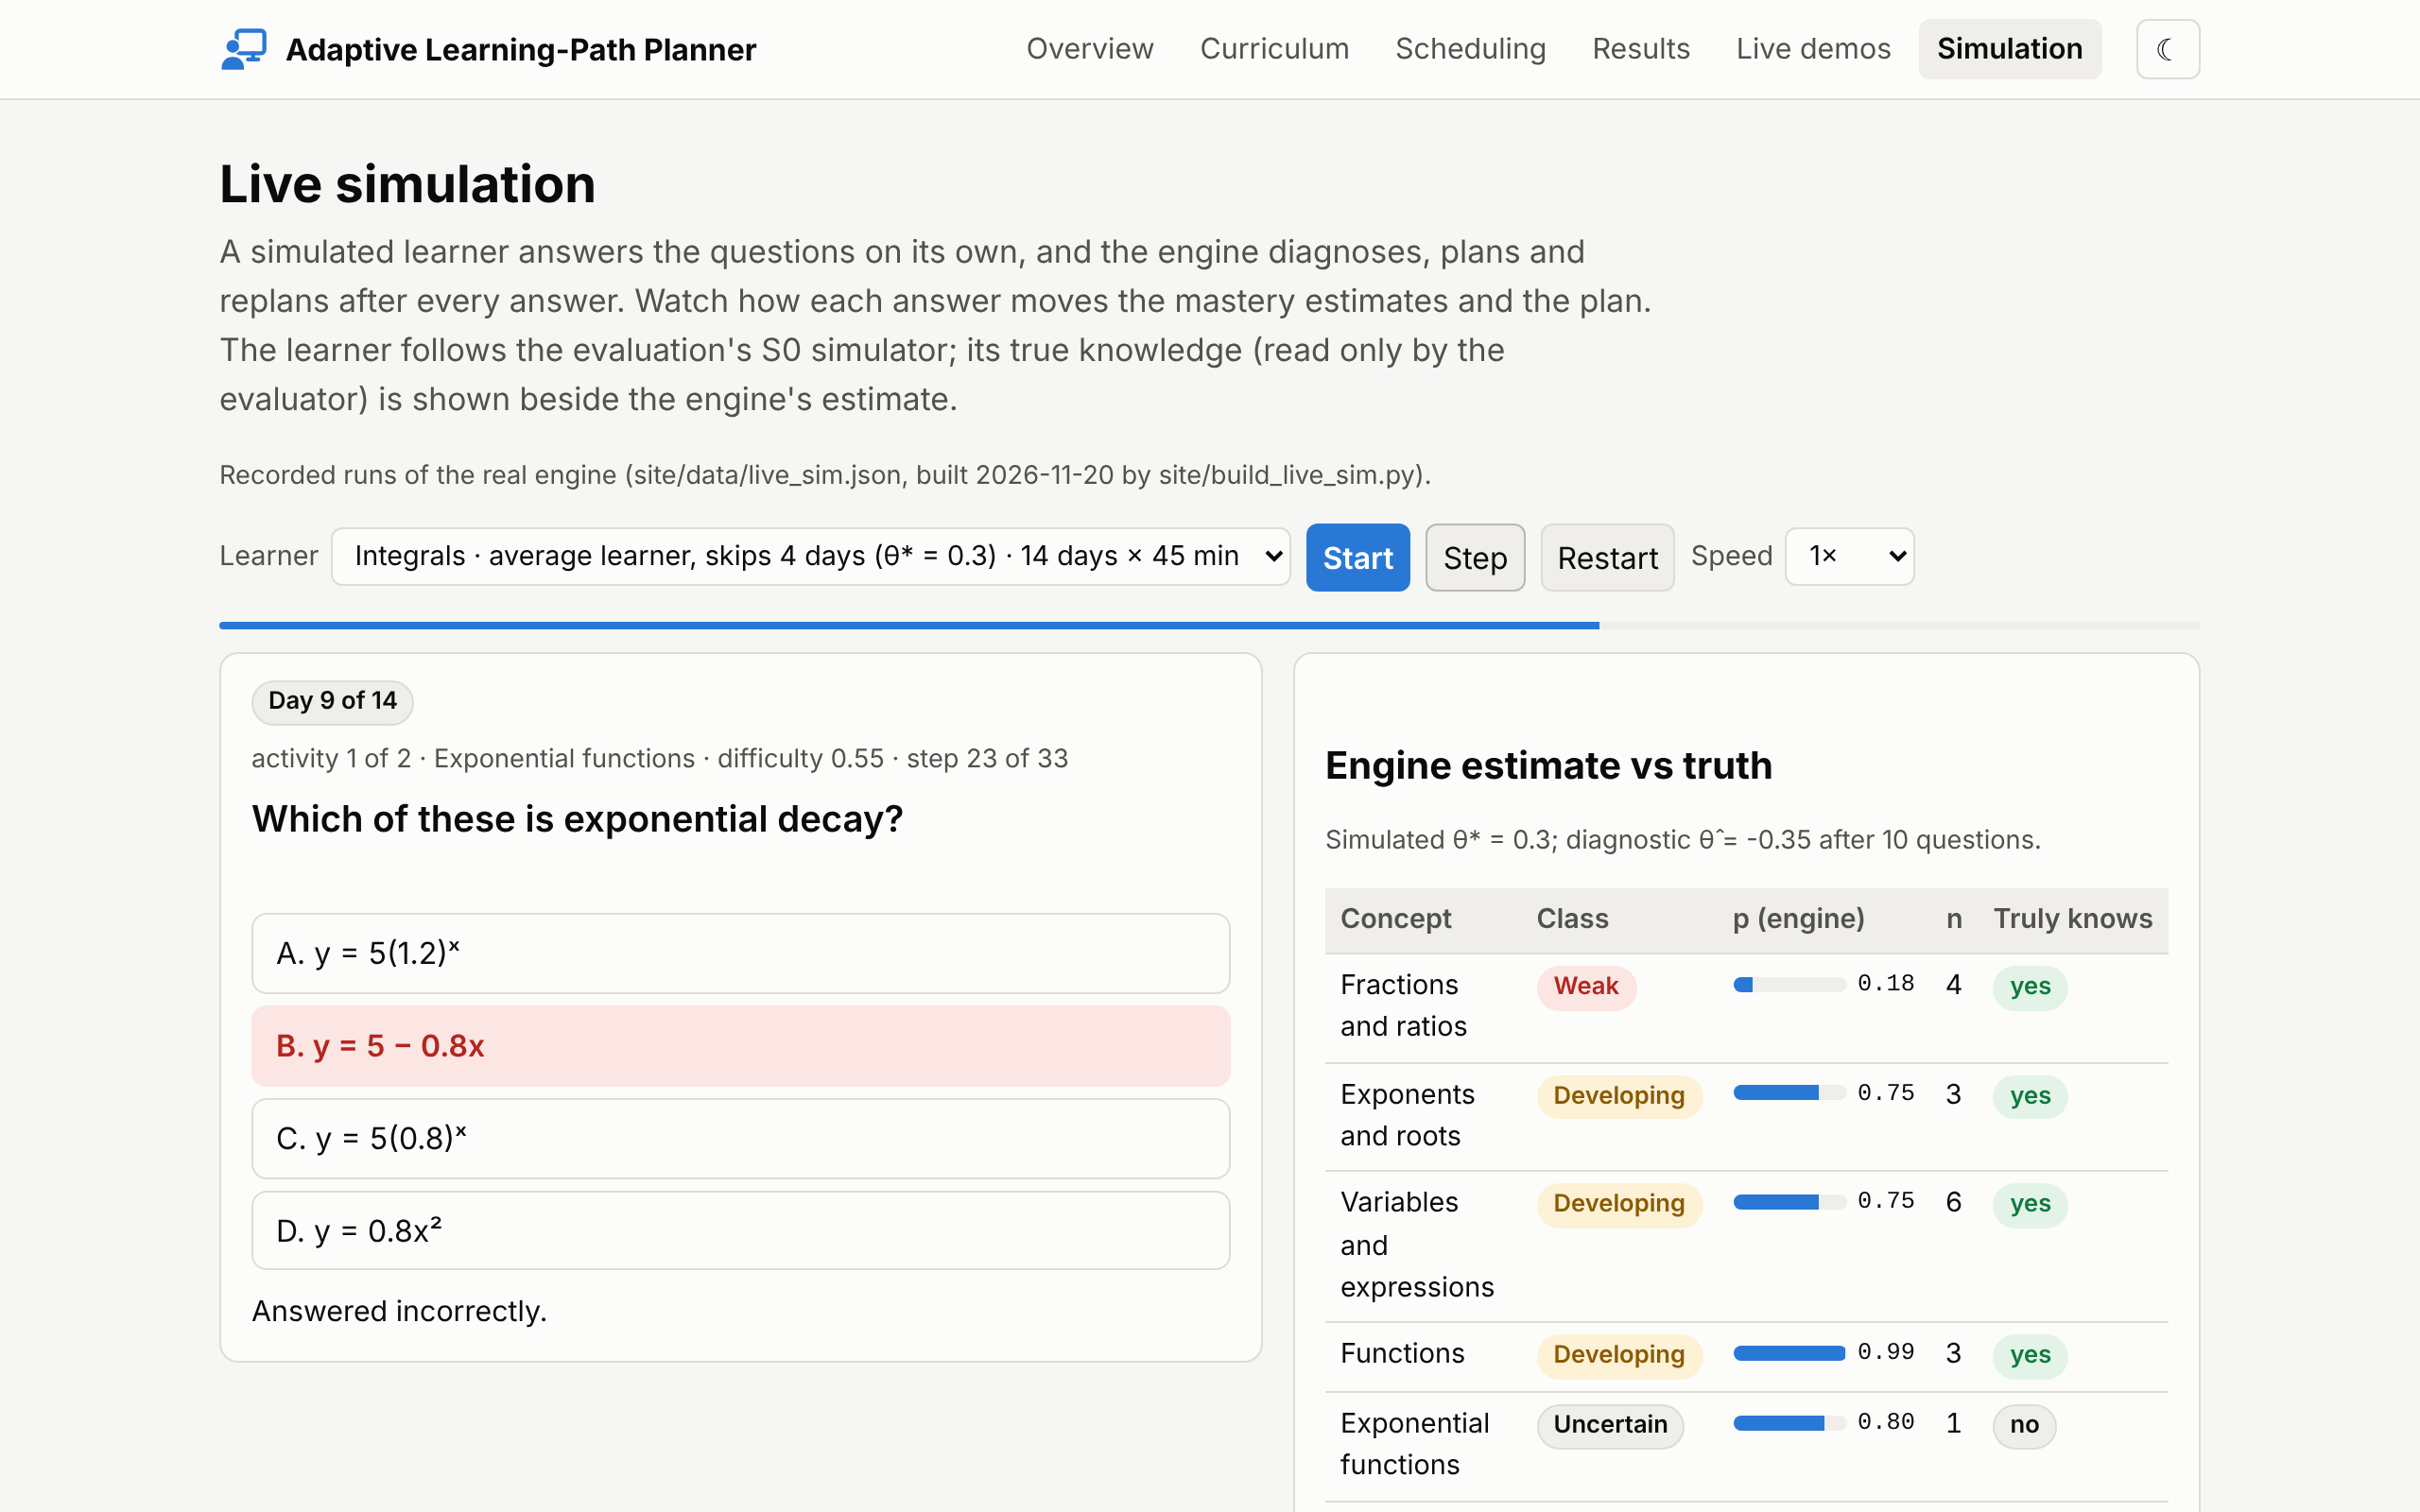
\includegraphics[width=0.86\textwidth]{images/ui_sim.png}
    \caption{Simulation page, recorded run ``average learner who skips 4 days'' (simulated $\theta^* = 0.3$), step 23 of 33: the learner answers an exponential-functions question incorrectly. The engine's class and $p$ sit beside what the simulator truly knows; e.g.\ Fractions is Weak ($p = 0.18$) although the learner knows it, after unlucky slips.}
\end{figure}
\begin{figure}[H]
    \centering
    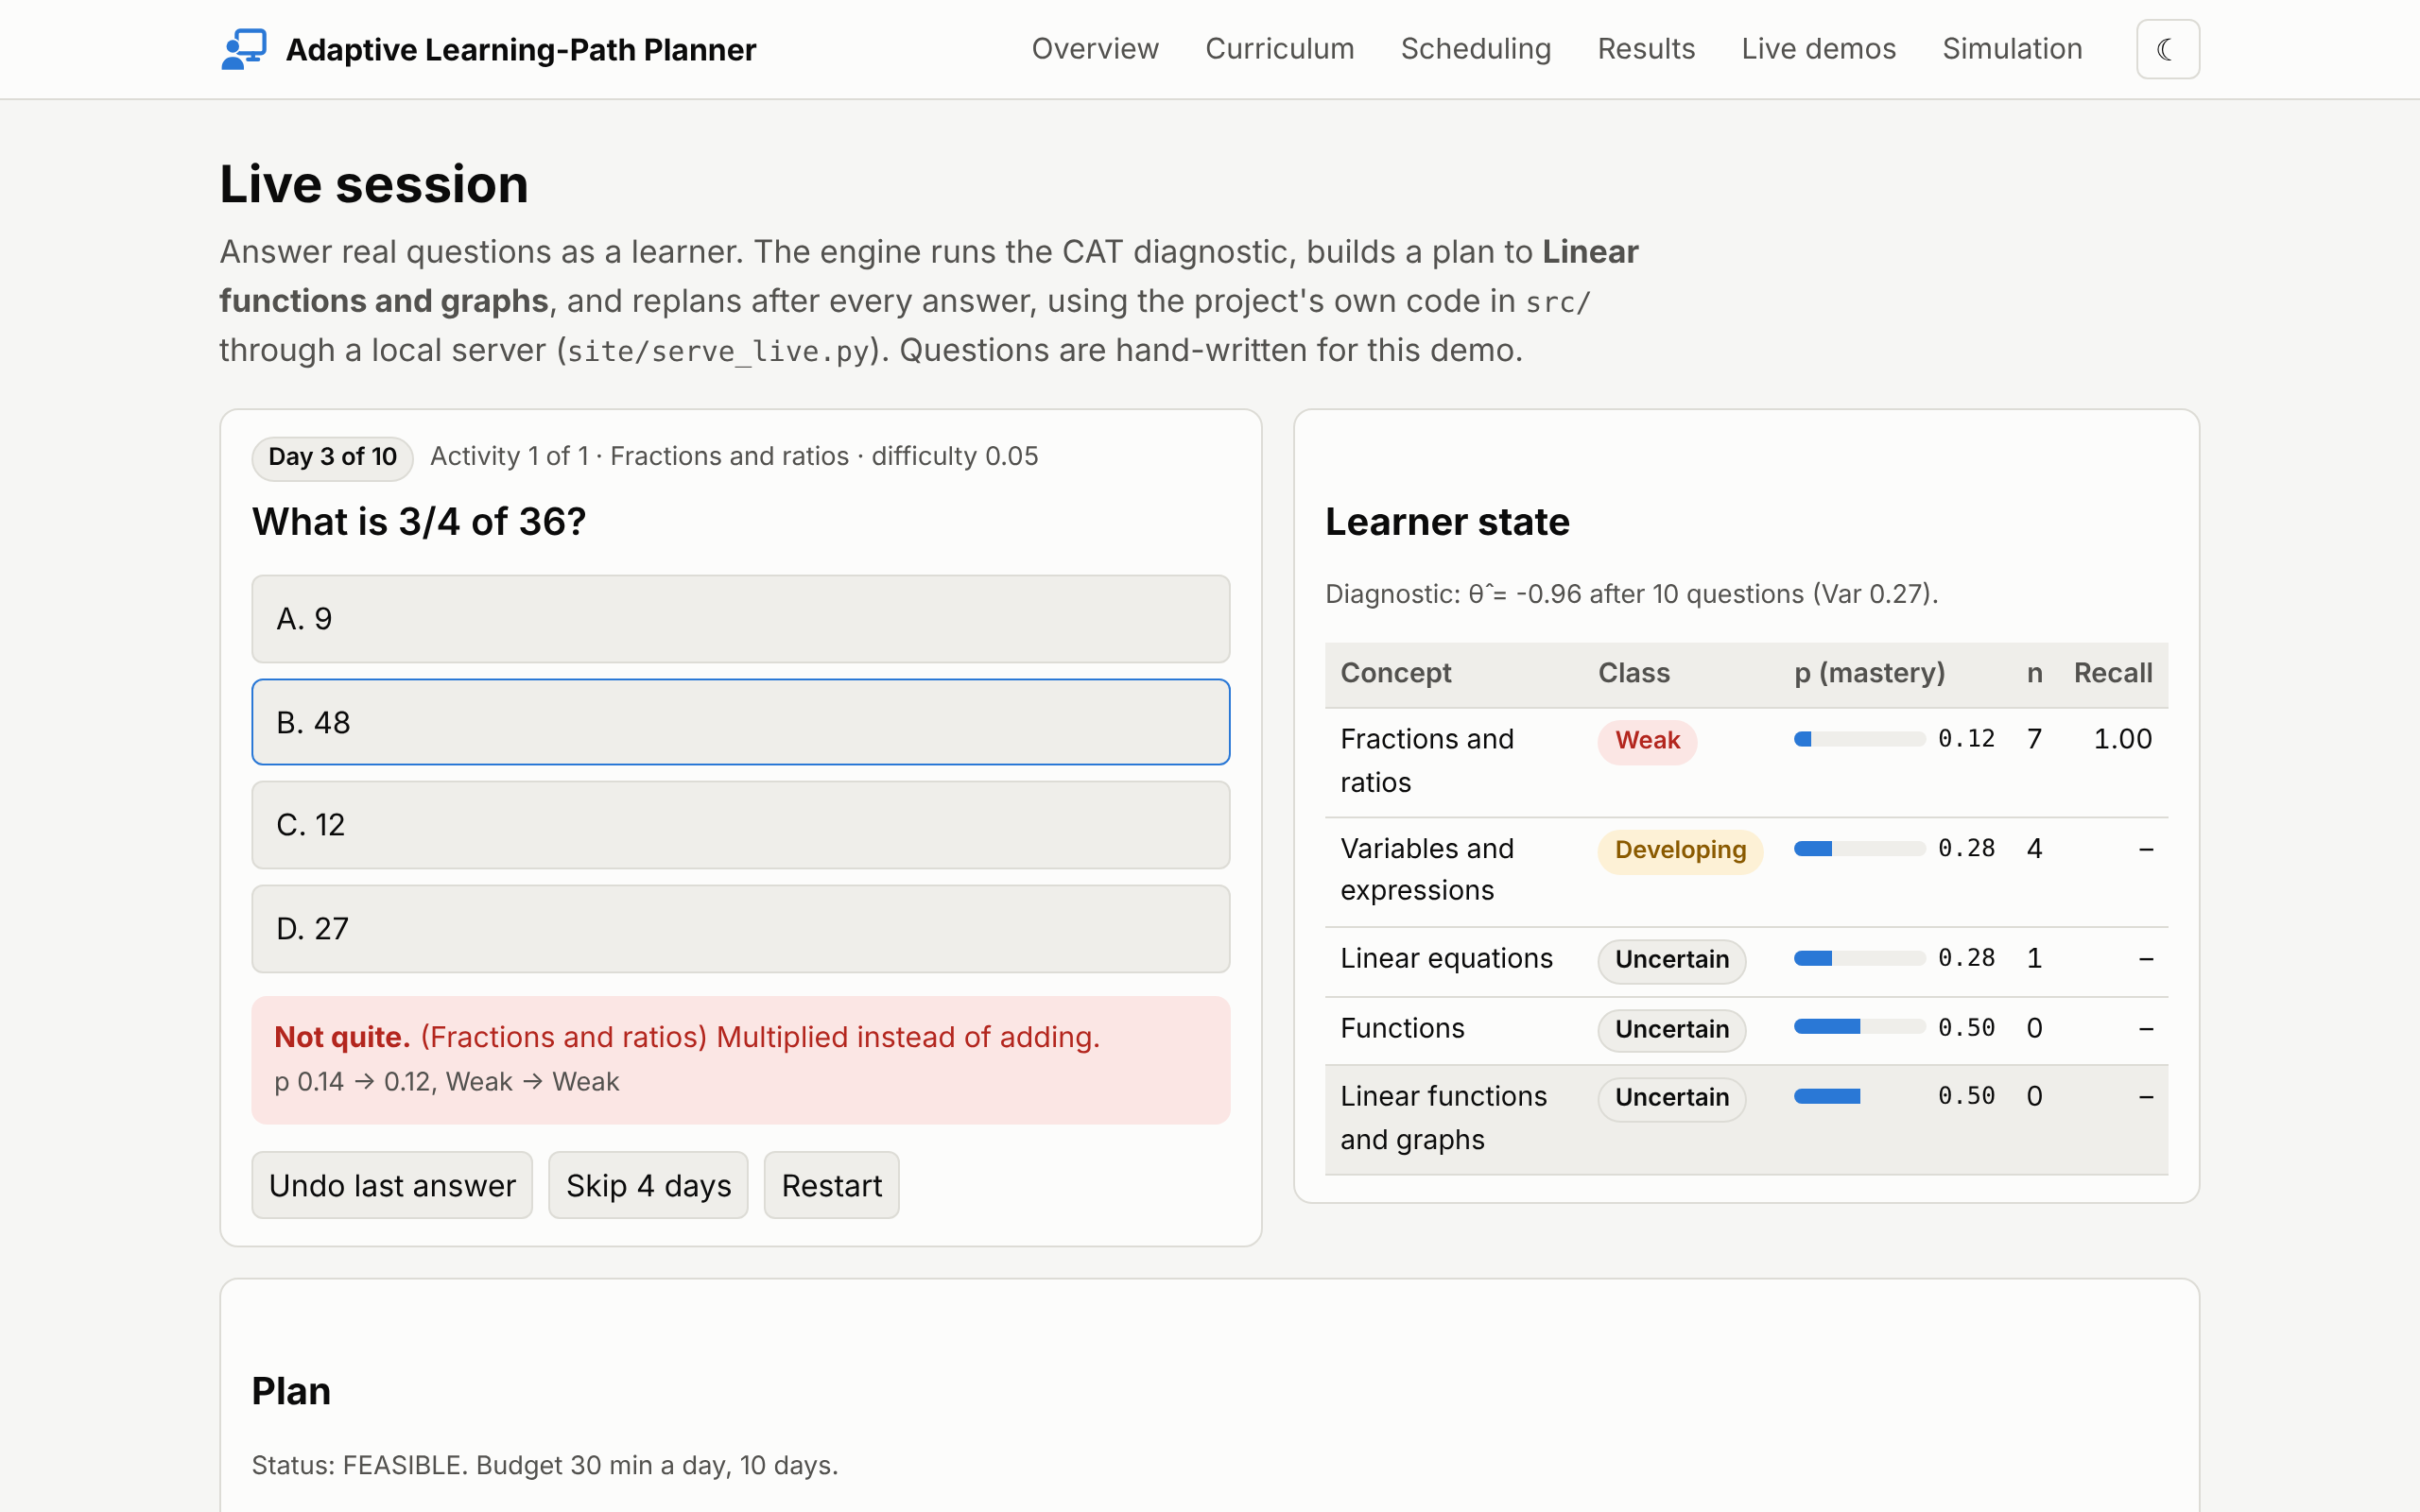
\includegraphics[width=0.86\textwidth]{images/ui_live.png}
    \caption{Live session page, a weak learner on day 3 (target Linear functions, 30 min/day): a wrong answer names the mistake, $p$ for Fractions falls from 0.14 to 0.12 and the engine keeps scheduling Fractions (\texttt{PRACTICE\_FOR\_EVIDENCE}) before its dependents. The engine state is a recorded response of the local server.}
\end{figure}
\vspace{0.2em}\noindent
\textbf{Limitations.} No accounts or saved learners; one event per replan; the live demos need internet access once; results pages show precomputed runs. The screenshots were captured from a local copy of the site at \cm{d974503} where the Pyodide CDN was unreachable, so the demos show the saved preset outputs (marked ``Saved output'' on the page); these are produced by the same code and match what the live engine returns for those presets.
\vspace{0.2em}\newline
\subsection{Reproducibility and Provenance}
Every run writes a manifest with the git SHA and dirty flag, timestamp, Python version, a SHA-256 hash of the resolved configuration, input paths and output checksums (\rf{src/provenance.py}). Evaluation outputs refuse to write under \texttt{evaluation/results/} from a dirty tree. \rf{scripts/clean_run.ps1} clones the repository fresh, installs pinned dependencies, runs the suite and the demo, slice and evaluate commands, and checks every artifact (M8-b). A GitHub Actions workflow runs pytest on Ubuntu with Python 3.11.

% ==================================================
\section{Methodology and Experiment Setup}
% ==================================================
\subsection{Evaluation Questions}
\textbf{Q1} Is the greedy planner close to optimal, and how fast is it?\\ \textbf{Q2} Does the CAT estimate ability better than fixed or random items?\\ \textbf{Q3} Does the adaptive system teach and retain more than static and greedy plans on the same learners?\\ \textbf{Q4} Does the result survive forgetting, a larger curriculum and a simulator that does not match the planner's model?\\ \textbf{Q5} Are the engine's mastery estimates calibrated?\\ \textbf{Q6} Do the hard constraints hold everywhere?\\ \textbf{Q7} (Week 8 extension) Does the engine's model fit real students, and does the result hold on learners calibrated to them?

\subsection{Simulated Learners}
{\small
\begin{longtable}{|L{2.47cm}|L{7.04cm}|L{5.52cm}|}
\caption{Simulator scenarios (\rf{src/simulation/simulator.py}). The planner sees only answers; latent state is read by the evaluator alone.}\\
\hline
\textbf{Scenario} & \textbf{Learner model} & \textbf{Bias} \\ \hline
\endfirsthead
\hline \textbf{Scenario} & \textbf{Learner model} & \textbf{Bias} \\ \hline
\endhead
S0 matched & BKT generator with the same slip, guess and learn parameters as the engine & Most favourable to the planner: learners behave exactly as it assumes \\ \hline
S1 forgetting & S0 plus daily forgetting $p_F = 0.05$ during study and over a 7-day delay & Planner does not model forgetting directly (B9) \\ \hline
S3 mismatched & PFA/logistic: accuracy $=\sigma(\beta_c + \gamma\cdot\text{successes} + \rho\cdot\text{failures} - \text{difficulty term})$; learning from practice counts & Rewards practice attempts, which favours the adaptive arm \\ \hline
S4 calibrated & BKT; each (learner, concept) draws slip, guess and learn from one of 53 per-skill fits on ASSISTments students (guess and slip $<0.5$); engine keeps its defaults (\rfx{src/simulation/calibrated.py}) & Learners differ from the planner's model; toy curriculum, no forgetting only \\ \hline
 \end{longtable}
}

\subsection{Arms}
{\small
\begin{longtable}{|L{3.6cm}|L{1.75cm}|L{2.2cm}|L{1.75cm}|C{1.2cm}|C{1.2cm}|C{1.25cm}|}
\caption{Evaluation arms (\rf{src/evaluation/integrated.py}).}\\
\hline
\textbf{Arm} & \textbf{Priors} & \textbf{Planner} & \textbf{Difficulty} & \textbf{Replan} & \textbf{Review} & \textbf{Remed.} \\ \hline
\endfirsthead
\hline \textbf{Arm} & \textbf{Priors} & \textbf{Planner} & \textbf{Difficulty} & \textbf{Replan} & \textbf{Review} & \textbf{Remed.} \\ \hline
\endhead
adaptive\_\allowbreak full & CAT ($n=k$) & replan & 2-up/1-down & on & on & on \\ \hline
static\_\allowbreak prerequisite\_\allowbreak order & CAT ($n=0$) & static topological & base & off & off & off \\ \hline
non\_\allowbreak adaptive\_\allowbreak greedy & CAT ($n=0$) & greedy score/min & base & off & off & off \\ \hline
non\_\allowbreak adaptive\_\allowbreak greedy\_\allowbreak best\_\allowbreak singleton & CAT ($n=0$) & greedy + fallback & base & off & off & off \\ \hline
ablation\_\allowbreak no\_\allowbreak diagnostic & cold start & replan & 2-up/1-down & on & on & on \\ \hline
ablation\_\allowbreak no\_\allowbreak replan & CAT & static & 2-up/1-down & off & off & off \\ \hline
ablation\_\allowbreak no\_\allowbreak difficulty\_\allowbreak step & CAT & replan & base & on & on & on \\ \hline
ablation\_\allowbreak no\_\allowbreak review & CAT & replan & 2-up/1-down & on & off & on \\ \hline
ablation\_\allowbreak no\_\allowbreak remediation & CAT & replan & 2-up/1-down & on & on & on$^*$ \\ \hline
\end{longtable}
}
{\footnotesize $^*$ Known defect B1: the remediation ablation does not actually disable remediation; remediation also never triggers in the loop (B2).}

\subsection{Workloads, Repeats and Metrics}
\begin{itemize}
    \item \textbf{Toy curriculum:} 4 concepts, target D (Division), 5 days $\times$ 10 min. \textbf{Maths curriculum:} 16 concepts, target Integrals, 10 days $\times$ 30 min.
    \item \textbf{Repeats:} 5 seeds (42, 101, 2024, 777, 999) $\times$ 200 learners $=$ 1,000 paired learners per arm per run. Scheduling: 250 instances, seeds 7, 17, 27, 37, 47 (50 each).
    \item \textbf{Metrics:} concepts mastered (latent, at the horizon); retained recall (share correct on $N=5$ fresh items per studied concept after a 7-day delay); no-plan days; prerequisite and budget violations, recounted independently of the planner; trace coverage; runtime p50/p95 per plan; diagnostic $|\hat\theta-\theta^*|$, concept Brier score and held-out log loss; engine mastery Brier score and 10-bin ECE; greedy/oracle score ratio.
    \item \textbf{Statistics:} per-learner paired differences; percentile bootstrap, $B = 1{,}000$; a claim only if the 95\% CI excludes zero.
    \item \textbf{Public data (Q7):} ASSISTments 2009--2010 corrected file, 346,860 rows; original questions, single-skill rows, first attempt per (student, problem), skills with $\geq 50$ students and $\geq 500$ rows: 196,143 answers, 3,958 students, 56 skills; split by student 70/15/15 (seed 20261119). pyBKT EM per skill on train students (5 restarts); prediction is the BKT forward pass on test students. S4 uses the toy S0 configuration (\rfx{experiments/w8_s4_assistments.yaml}).
    \item \textbf{Environment:} Windows laptop, Python 3.11 virtual environment, pinned requirements; runtimes come from one machine and one run.
\end{itemize}

\subsection{How to Reproduce}
{\footnotesize
\begin{verbatim}
pip install -r requirements.txt
python -m pytest -q                                                  # 303 passed
python -m src.planning.benchmark                                     # Q1
python -m src.evaluation.diagnostic_comparison \
       --config experiments/w4_comparison.yaml                       # Q2
python -m src.evaluation.integrated --config experiments/w8_final.yaml    --out out/s0
python -m src.evaluation.integrated --config experiments/w8_final_s1.yaml --out out/s1
python -m src.evaluation.integrated --config experiments/w8_maths_s0.yaml --out out/m0
#   (also experiments/w8_maths_s3.yaml and experiments/w8_toy_s3.yaml)
python scripts/w7_pooled_s0.py out/s0 adaptive_full:static_prerequisite_order
powershell scripts/clean_run.ps1                                     # clean-clone audit
python scripts/assistments_prepare.py   # Q7: needs the raw ASSISTments file in data/raw/
python scripts/assistments_fit_bkt.py
python -m src.evaluation.integrated --config experiments/w8_s4_assistments.yaml --out out/s4
python scripts/w8_s4_compare.py
\end{verbatim}
}
% ==================================================
\section{Results, Observations and Analysis}
% ==================================================
Raw outputs for every number below are in \rd{evaluation/results/w8/final_v2} (per-seed CSVs, summaries, manifests, \texttt{pooled\_*.txt}, \texttt{before\_after.txt}) unless another file is named. ``\nd'' means no difference shown.

\subsection{Scheduling Quality and Runtime (Q1)}
{\small
\begin{longtable}{|L{4.08cm}|C{1.58cm}|C{1.39cm}|C{1.39cm}|C{2.23cm}|C{3.06cm}|}
\caption{Greedy vs exact oracle on 250 synthetic instances (\rf{evaluation/results/w7/improvement/scheduling/summary.md}).}\\
\hline
\textbf{Policy} & \textbf{Mean ratio} & \textbf{5th pct} & \textbf{Min} & \textbf{Below 0.95} & \textbf{Runtime p50 / p95} \\ \hline
\endfirsthead
\hline \textbf{Policy} & \textbf{Mean ratio} & \textbf{5th pct} & \textbf{Min} & \textbf{Below 0.95} & \textbf{Runtime p50 / p95} \\ \hline
\endhead
Greedy score-per-minute & 0.9737 & 0.8270 & 0.2143 & 35 / 250 & 0.022 / 0.066 ms \\ \hline
Greedy + best-singleton & 0.9814 & 0.8548 & 0.5000 & 25 / 250 & 0.027 / 0.073 ms \\ \hline
\end{longtable}
}
\begin{figure}[H]
    \centering
    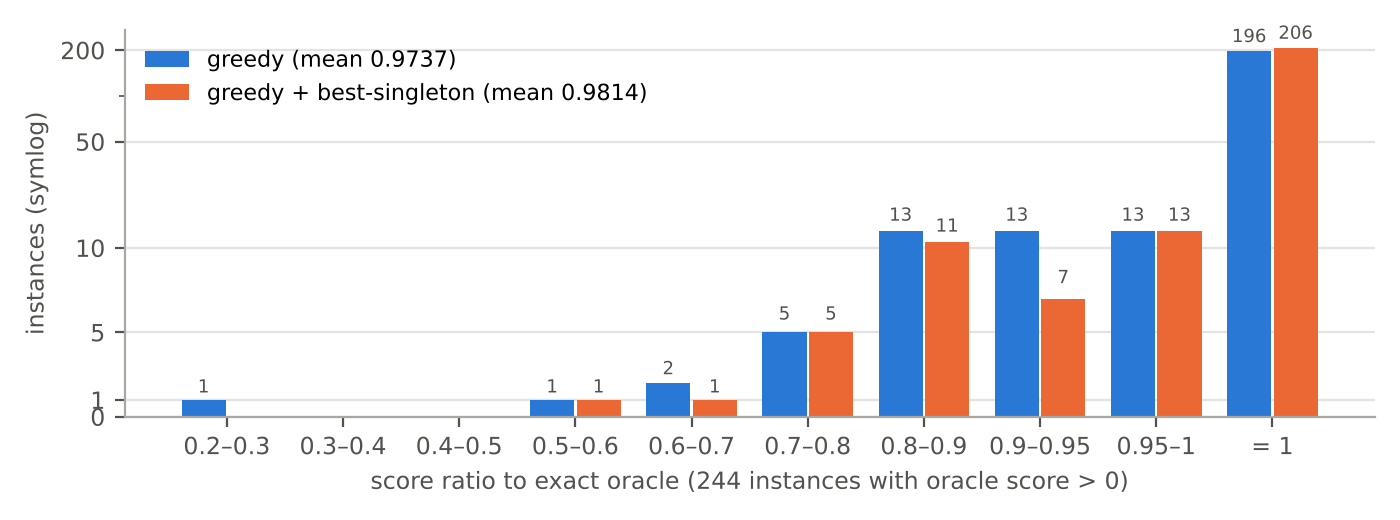
\includegraphics[width=0.9\textwidth]{images/chart_ratio.png}
    \caption{Distribution of greedy/oracle score ratios (244 instances with oracle score $>0$). The fallback moves 10 instances to the optimum and lowers none.}
\end{figure}
The paired difference is $+0.0077$ [0.0018, 0.0159]: the fallback is better. The mean exceeds the 0.95 target, but individual plans can be far from optimal: instance 215 scores 0.214 with greedy and the hand-made 12/18 case stays at 0.667 with both policies, so no worst-case guarantee is claimed (B8). Mean oracle runtime is 0.24\,ms on these small instances. Inside the closed loop (seed-42 summaries in \texttt{final\_v2}) one adaptive plan takes 13.7 / 24.1\,ms (p50 / p95) on the toy curriculum and 78.3 / 134.1\,ms on the maths curriculum, against 0.56 / 0.83\,ms and 2.8 / 3.8\,ms for the static planner.

\subsection{Diagnostic Accuracy (Q2)}
\label{sec:diag}
{\small
\begin{longtable}{|L{2.77cm}|L{3.97cm}|L{3.88cm}|L{3.97cm}|}
\caption{CAT vs fixed-order vs random items, 1,000 paired learners, all capped at 10 items (\rf{evaluation/results/w8/diagnostic_comparison/summary.md}). Lower is better.}\\
\hline
\textbf{adaptive $-$ X} & $|\hat\theta - \theta^*|$ & \textbf{Concept Brier} & \textbf{Held-out log loss} \\ \hline
\endfirsthead
\hline \textbf{adaptive $-$ X} & $|\hat\theta - \theta^*|$ & \textbf{Concept Brier} & \textbf{Held-out log loss} \\ \hline
\endhead
fixed order & $-0.064$ [$-0.092$, $-0.038$] \textbf{better} & $-0.003$ [$-0.007$, $+0.001$] \nd & $-0.009$ [$-0.016$, $-0.003$] \textbf{better} \\ \hline
random & $-0.082$ [$-0.110$, $-0.056$] \textbf{better} & $-0.006$ [$-0.010$, $-0.002$] \textbf{better} & $-0.016$ [$-0.024$, $-0.008$] \textbf{better} \\ \hline
\end{longtable}
}
The CAT is more accurate in 5 of 6 comparisons; Brier score against fixed order shows no difference. The gains are small, and because the variance stop never fires with a 24-item bank (B5), the CAT is not shorter than the baselines.

\subsection{Integrated Outcomes (Q3)}
{\footnotesize\setlength{\tabcolsep}{4pt}
\begin{longtable}{|L{1.2cm}|L{2.5cm}|C{1.05cm}|C{1.05cm}|C{1.05cm}|C{3.6cm}|C{3.6cm}|}
\caption{Concepts mastered and retained recall, adaptive\_full vs both baselines, 1,000 paired learners per cell.}\\
\hline
\textbf{Scen.} & \textbf{Metric} & \textbf{Static} & \textbf{Greedy} & \textbf{Adapt.} & \textbf{Adaptive $-$ static [95\% CI]} & \textbf{Adaptive $-$ greedy [95\% CI]} \\ \hline
\endfirsthead
\hline \textbf{Scen.} & \textbf{Metric} & \textbf{Static} & \textbf{Greedy} & \textbf{Adapt.} & \textbf{Adaptive $-$ static [95\% CI]} & \textbf{Adaptive $-$ greedy [95\% CI]} \\ \hline
\endhead
Toy S0 & mastered (of 4) & 2.036 & 2.036 & 2.092 & $+0.056$ [0.040, 0.074] & $+0.056$ [0.040, 0.074] \\
 & retained recall & 0.636 & 0.636 & 0.660 & $+0.024$ [0.017, 0.032] & $+0.024$ [0.017, 0.032] \\ \hline
Toy S1 & mastered (of 4) & 1.587 & 1.594 & 1.632 & $+0.045$ [0.022, 0.064] & $+0.038$ [0.000, 0.075] \nd \\
 & retained recall & 0.516 & 0.518 & 0.531 & $+0.015$ [0.007, 0.024] & $+0.013$ [0.003, 0.023] \\ \hline
Toy S3 & mastered (of 4) & 2.334 & 2.334 & 2.451 & $+0.117$ [0.096, 0.139] & $+0.117$ [0.096, 0.139] \\ \hline
Maths S0 & mastered (of 16) & 6.254 & 6.337 & 6.348 & $+0.094$ [0.047, 0.140] & $+0.011$ [$-0.031$, 0.059] \nd \\
 & retained recall & 0.589 & 0.603 & 0.684 & $+0.095$ [0.087, 0.103] & $+0.081$ [0.074, 0.089] \\ \hline
Maths S3 & mastered (of 16) & 6.776 & 7.098 & 7.503 & $+0.727$ [0.631, 0.824] & $+0.405$ [0.310, 0.500] \\
 & retained recall & -- & -- & 0.864 & $+0.104$ [0.100, 0.109] & $+0.081$ [0.077, 0.085] \\ \hline
\end{longtable}
}
\begin{figure}[H]
    \centering
    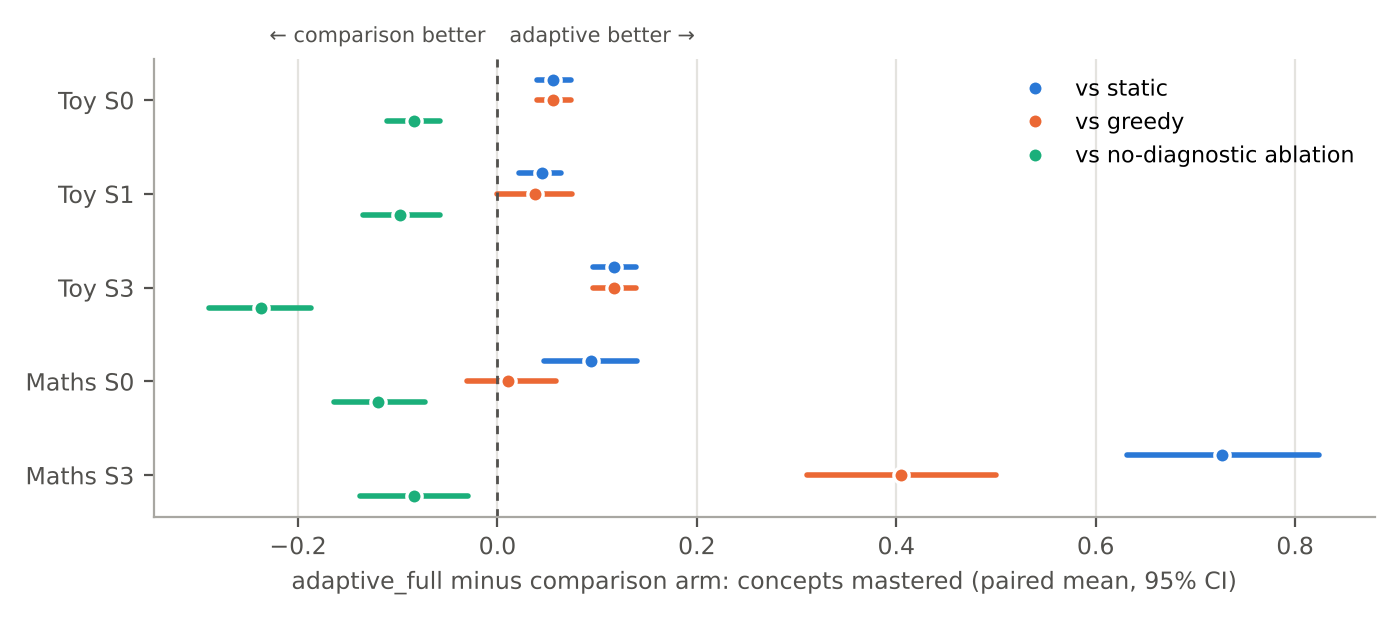
\includegraphics[width=0.92\textwidth]{images/chart_paired.png}
    \caption{Paired differences in concepts mastered (adaptive\_full minus each arm), 95\% bootstrap CIs. Blue and orange: the two baselines. Aqua: the cold-start ablation, which now does better than the full system (Section~\ref{sec:failures}).}
\end{figure}
\textbf{Observations.} The adaptive arm beats static in every scenario and on both outcomes. Against greedy it wins on mastery in 3 of 5 runs and on retained recall in all runs. On the matched simulator the effect is small ($+0.056$ of 4 concepts, about 3\%). Under S1 forgetting costs every arm about 0.45 concepts and the adaptive advantage shrinks. The largest effects are under S3, which rewards practice directly.
\vspace{0.2em}\newline
\textbf{Ablations.} On toy S0: \texttt{no\_replan} reaches 2.035 (adaptive better by 0.057); \texttt{no\_difficulty\_step}, \texttt{no\_review} and \texttt{no\_remediation} equal adaptive\_full on mastery; \texttt{no\_diagnostic} reaches 2.176, better than adaptive ($-0.084$ [$-0.111$, $-0.058$]). Under S1 only, the review ablation is slightly better ($-0.017$ [$-0.033$, $-0.001$]). So only the whole adaptive arm can be credited against the baselines, not its individual parts (B3).

\subsection{Robustness (Q4)}
{\small
\begin{longtable}{|L{4.35cm}|C{5.34cm}|C{5.34cm}|}
\caption{Adaptive $-$ static, concepts mastered: curriculum $\times$ simulator (\rf{evaluation/results/w8/final_v2/before_after.txt}).}\\
\hline
 & \textbf{S0 matched} & \textbf{S3 mismatched} \\ \hline
\endfirsthead
\hline & \textbf{S0 matched} & \textbf{S3 mismatched} \\ \hline
\endhead
Toy, 4 concepts & $+0.056$ [0.040, 0.074] & $+0.117$ [0.096, 0.139] \\ \hline
Maths, 16 concepts & $+0.094$ [0.047, 0.140] & $+0.727$ [0.631, 0.824] \\ \hline
\end{longtable}
}
The advantage over static holds in all four cells. Because S3 rewards the adaptive arm's extra practice, ``survives a mismatched simulator'' is supported; ``larger with real learners'' is not.

\subsection{Calibration of Mastery Estimates (Q5)}
\label{sec:calib}
\noindent\begin{minipage}[t]{0.56\textwidth}
\vspace{0pt}
{\small
\begin{tabular}{|L{1.6cm}|L{3.4cm}|L{2.1cm}|}
\hline
\textbf{Run} & \textbf{adaptive\_full Brier [95\% CI] / ECE} & \textbf{no-diagnostic} \\ \hline
Toy S0 & 0.136 [0.129, 0.143] / 0.082 & 0.146 / 0.064 \\ \hline
Toy S1 & 0.196 [0.187, 0.203] / 0.163 & 0.189 / 0.145 \\ \hline
Toy S3 & 0.167 [0.158, 0.176] / 0.089 & 0.142 / 0.079 \\ \hline
Toy S4 & 0.161 [0.154, 0.168] / 0.114 & 0.182 / 0.124 \\ \hline
Maths S0 & 0.190 [0.187, 0.193] / 0.166 & 0.187 / 0.141 \\ \hline
Maths S3 & 0.188 [0.185, 0.192] / 0.155 & 0.191 / 0.156 \\ \hline
\end{tabular}
}
\captionof{table}{Mastery Brier score and ECE of the engine's $p$ at the horizon against latent mastery.}
\vspace{4pt}
Static and greedy arms never update $p$, so calibration does not apply to them. High-confidence bins are well calibrated ($p \approx 0.93 \rightarrow$ 99.5\% mastered); the worst bin is $p \approx 0.5$, which holds concepts the learner never practised. Calibration degrades under forgetting, on the larger curriculum, and when learners' parameters differ from the engine's (S4).
\end{minipage}\hfill
\begin{minipage}[t]{0.41\textwidth}
\vspace{0pt}
\centering
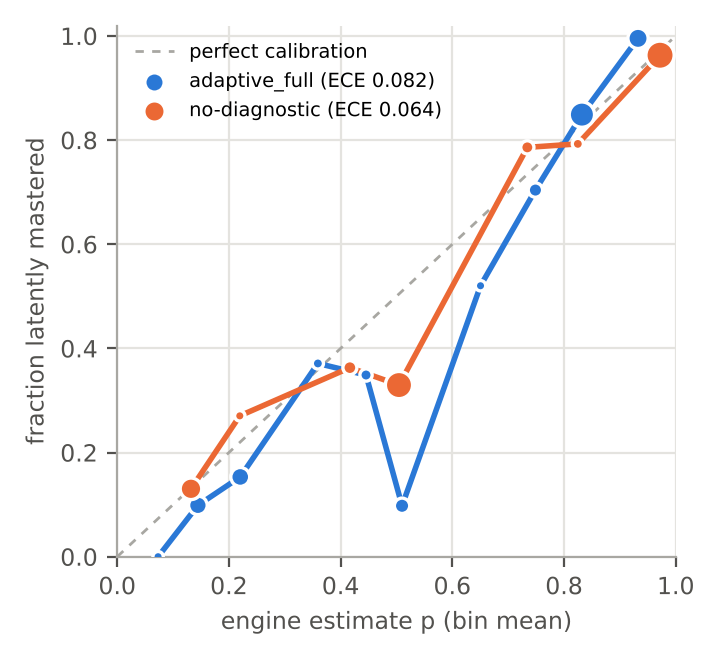
\includegraphics[width=\textwidth]{images/chart_reliability.png}
\captionof{figure}{Reliability diagram, toy S0 (dot size = number of learner $\times$ concept pairs).}
\end{minipage}

\subsection{Hard Constraints (Q6)}
0 prerequisite violations and 0 budget violations in all 9 arms of all 5 final runs (45,000 learner-runs), and in S4 (9,000 more), recounted independently of the planner; trace coverage is 100\% for the four primary arms (the harness does not record coverage for ablations).

\subsection{Public Data: BKT on Real Students and Calibrated Learners (Q7)}
\label{sec:public}
\textbf{Held-out prediction} (\rfx{evaluation/results/w8/assistments_bkt/metrics.txt}, 27,665 answers from 593 test students):
{\small
\begin{longtable}{|L{5.6cm}|C{1.5cm}|C{1.5cm}|C{1.5cm}|C{1.5cm}|C{1.5cm}|}
\hline
\textbf{Model} & \textbf{AUC} & \textbf{RMSE} & \textbf{Acc.} & \textbf{Log loss} & \textbf{ECE} \\ \hline
\endfirsthead
\hline \textbf{Model} & \textbf{AUC} & \textbf{RMSE} & \textbf{Acc.} & \textbf{Log loss} & \textbf{ECE} \\ \hline
\endhead
BKT fitted per skill (train students) & \textbf{0.714} & \textbf{0.441} & \textbf{0.707} & \textbf{0.573} & 0.017 \\ \hline
BKT, engine defaults (0.10 / 0.25 / 0.10, prior 0.5) & 0.681 & 0.457 & 0.696 & 0.613 & 0.069 \\ \hline
Per-skill training correct-rate & 0.621 & 0.464 & 0.662 & 0.621 & 0.009 \\ \hline
Majority class & 0.500 & 0.584 & 0.659 & 4.710 & 0.341 \\ \hline
\caption{BKT on held-out ASSISTments 2009--2010 students.}
\end{longtable}
}
Fitted minus default log loss per test student: $-0.0288$ [$-0.0378$, $-0.0192$], fitted better. This meets ADR-001's revisit trigger; the engine keeps its defaults in the delivered configuration, since switching after seeing results would be an unregistered change (ADR-023). The fitted BKT has lower RMSE than the per-skill average in 48 of 56 skills. Real students slip about twice as often as assumed and guess less (Figure~\ref{fig:params}).
\begin{figure}[H]
    \centering
    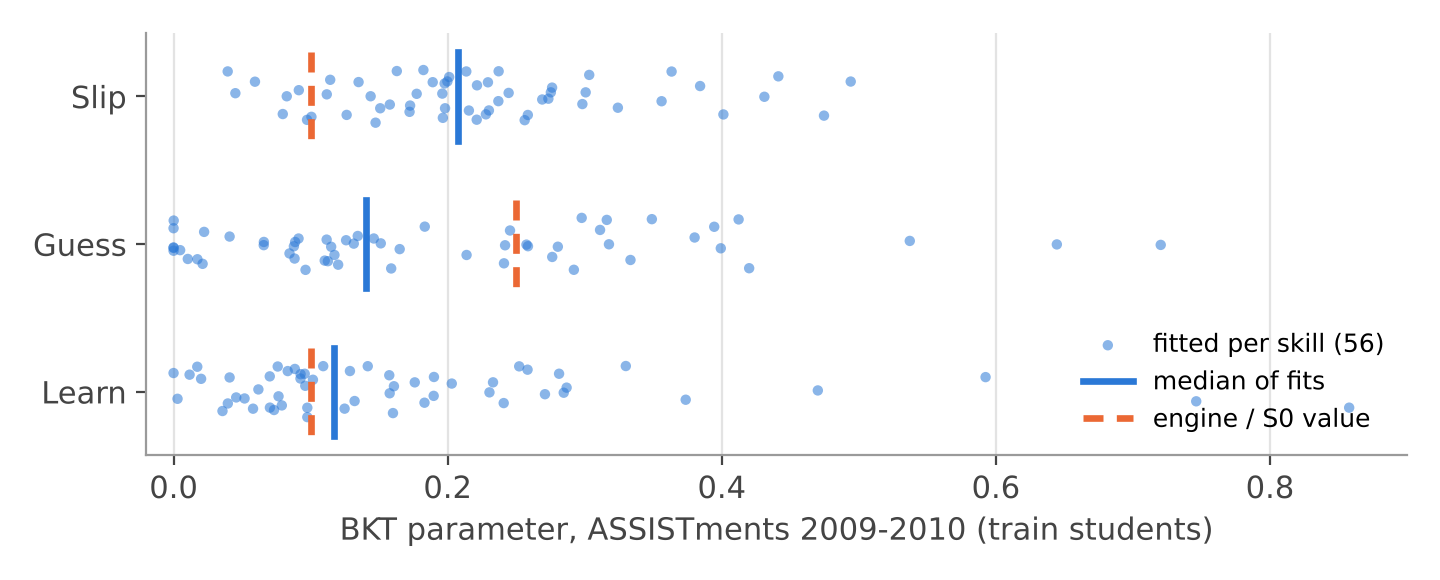
\includegraphics[width=0.84\textwidth]{images/chart_assistments_params.png}
    \caption{Per-skill BKT fits on ASSISTments train students against the single value the engine and S0 assume. Median slip 0.207 (assumed 0.10), guess 0.140 (0.25), learn 0.117 (0.10). A few fits are poorly identified (guess up to 0.72); S4 excludes the 3 with guess or slip $\geq 0.5$.}
    \label{fig:params}
\end{figure}
\textbf{S4: the integrated evaluation on calibrated learners} (\rfx{evaluation/results/w8/final_v2/s4_vs_s0.txt}). S4 has the same configuration as final\_v2 S0 (5 seeds $\times$ 200 learners) except that each learner's per-concept parameters come from the fits. A second run reproduced all five per-seed CSVs exactly, apart from runtimes.
\begin{figure}[H]
    \centering
    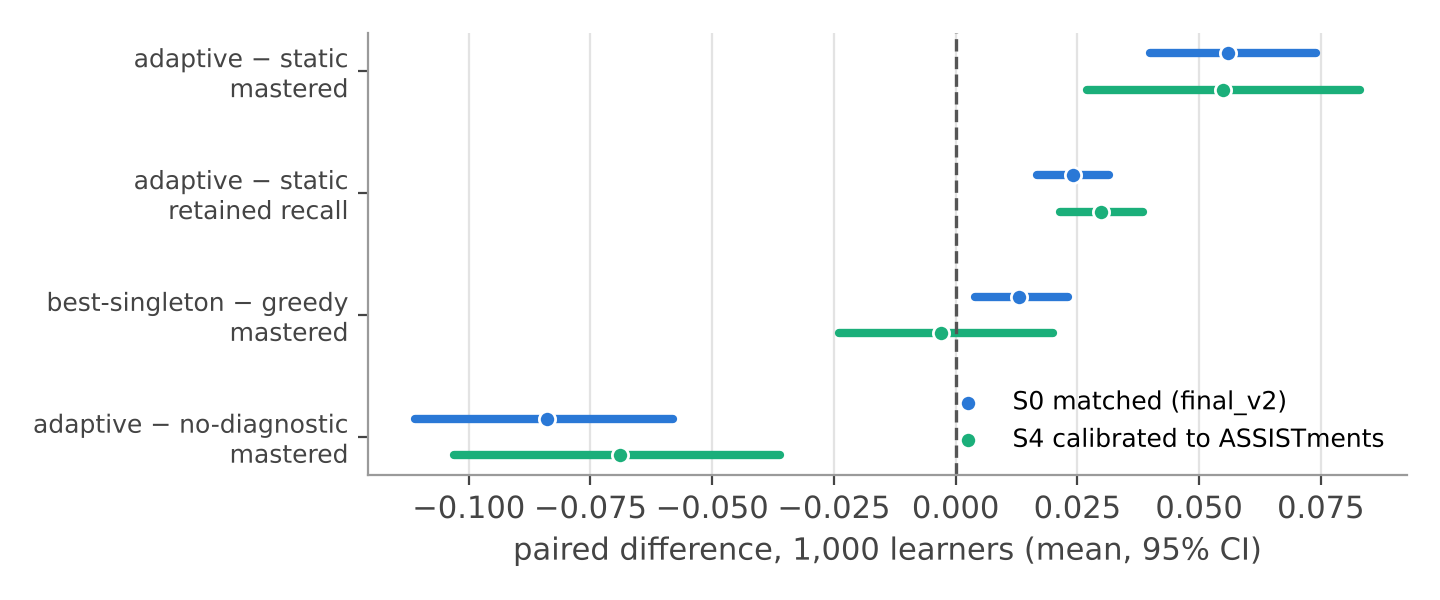
\includegraphics[width=0.84\textwidth]{images/chart_s4.png}
    \caption{Paired differences, S0 against S4 (1,000 learners each).}
\end{figure}
\textbf{Observations.}
\begin{itemize}
    \item \textbf{The headline claim holds:} adaptive beats static and greedy on mastery ($+0.055$ [0.027, 0.083]) and retained recall ($+0.030$ [0.021, 0.039]).
    \item \textbf{B12 is not an artifact of the matched simulator:} the cold-start ablation is still better ($-0.069$ [$-0.103$, $-0.036$]).
    \item \textbf{Calibration costs:} the engine's mastery calibration is worse (Brier 0.161 against 0.136), the cost of keeping its defaults.
    \item \textbf{The best-singleton gain is gone,} as under S1.
\end{itemize}
Not supported: real learners using the planner, curriculum structure from data (ASSISTments has no prerequisites), fitted HLR, and S4 under forgetting or on the maths curriculum.

\subsection{Failures and Edge Cases}
\label{sec:failures}
\begin{itemize}
    \item \textbf{Planned reviews were logged as done (B14, fixed 20 Nov).} When \texttt{replan} packed a due review into a future day, it immediately recorded a correct review at that day in the shared review log (\rf{src/planning/replan.py}), so a later replan or a missed day saw a fresh review and dropped it. Reproduction (\rfx{scripts/w8_b14_planned_reviews.py}): a Mastered concept practised on day 1 is planned for review on days 5, 9, 13 and 17; after missed days 3--8 the day-9 plan had no review, although true recall is 0.673 $<0.85$. \textbf{Fix} (\cm{03fd8ce}): planned reviews go into a planning copy of the log, and the returned log keeps only attempts that happened; the day-9 plan now reviews on days 9, 13 and 17 (\rfm{tests/test_w8_b14_review_log.py}). \textbf{Effect:} all six integrated scenarios were re-run with the same configurations and seeds (\rfm{evaluation/results/w8/final_v3/b14_before_after.txt}). adaptive\_full's mean mastery changed by at most 0.002 concepts and retained recall by at most 0.0011, every after$-$before 95\% interval contains 0, and adaptive$-$static moved by at most 0.002 concepts. All reported numbers therefore stand (they are the pre-fix final\_v2 runs). B14 was not why the review ablation rarely differs: adaptive$-$no-review is 0.000 in five runs and $-0.019$ $[-0.034, -0.003]$ under S1 ($-0.017$ before the fix).
    % \item \textbf{The diagnostic now lowers mastery (open, B12).} After B10 made diagnostic answers count as evidence, the cold-start ablation beats adaptive\_full in all five runs ($-0.084$ to $-0.237$ concepts). Observed mechanism: one $\hat\theta$ gives every probed concept the same $p$, and even an all-correct diagnostic reaches only $p \approx 0.76 < 0.85$, so probed concepts start as Developing or Weak rather than Mastered and lose the practice-for-evidence sessions that cold-start Uncertain concepts get. Why this lowers mastery was not tested; no code was changed to recover the earlier numbers.
    \item \textbf{Deadline-infeasible days.} 623 of 5,000 adaptive days on toy S0 and 5,751 of 10,000 on maths S0 cannot reach the target by the deadline. The planner returns the proof and a best-effort plan, so these are not idle days.
    \item \textbf{History: adaptive was once worse than static.} In Week 5 adaptive lost to static ($-0.080$); in Week 7, 4,000 of 5,000 adaptive days had no plan because completed-but-Uncertain prerequisites blocked their dependents. The deadlock fix moved adaptive $-$ static from $-0.102$ to $+0.140$ (\rf{docs/w7/deadlock_fix_results.md}); the later B10 fix reduced it to $+0.056$.
    \item \textbf{Edge cases covered by tests.} Cyclic, self-loop, missing-node and non-finite graphs are rejected; a block longer than the budget is proved infeasible; a missed day keeps completed work; a budget cut gives a valid plan or a structured infeasibility trace; an Uncertain prerequisite never unlocks a dependent; alternating answers stay Developing; the planner cannot import latent state.
\end{itemize}

% ==================================================
\section{Milestone Verification Matrix}
% ==================================================
Full criteria are in \rf{docs/ACCEPTANCE_GROUPS.md}. Recorded suite on 14 November (\cm{d974503}): \textbf{299 passed} on Windows, Python 3.11 (\rf{weekly/W8.md}); 303 after the S4 tests were added (20 November). Rows without a group ID are requirements from the brief verified by experiment.

{\small
\begin{longtable}{|C{1.12cm}|C{0.87cm}|L{3.65cm}|L{3.47cm}|C{1.13cm}|L{3.65cm}|}
\caption{Verification matrix.}\\
\hline
\textbf{Mile.} & \textbf{Test} & \textbf{Expected} & \textbf{Observed} & \textbf{Status} & \textbf{Evidence} \\ \hline
\endfirsthead
\hline \textbf{Mile.} & \textbf{Test} & \textbf{Expected} & \textbf{Observed} & \textbf{Status} & \textbf{Evidence} \\ \hline
\endhead
M1 & M1-a & Malformed graphs rejected (6 checks) & Rejected with error codes & Pass & \rf{tests/test_m1_curriculum_graph.py} \\ \hline
M1 & M1-b & BKT matches pyBKT 1.4.3 within $10^{-4}$ & Parity on all sequences & Pass & \rf{tests/test_m1_bkt_parity.py} \\ \hline
M1 & M1-c & Uncertain if $n<3$ or $\sigma^2>0.05$; window gate & Boundary tests pass & Pass & \rf{tests/test_m1_learner_state.py} \\ \hline
M1 & M1-d & Zero prerequisite violations & 0 in 45,000 learner-runs & Pass & \rf{tests/test_m3_states_feasibility.py} \\ \hline
M2 & M2-a & Max-information selection; stop at Var $\leq 0.15$ or 10 items & Selection correct; variance stop never fires (B5) & Pass$^*$ & \rf{tests/test_m2_adaptive_diagnostic.py} \\ \hline
M2 & M2-b & $\hat\theta \rightarrow$ concept priors; unprobed $=$ Beta(1,1) & Implemented incl.\ ADR-009 amendment & Pass & \rf{tests/test_w8_diagnostic_prior.py} \\ \hline
M2 & -- & CAT compared with fixed and random & Better in 5 of 6 paired comparisons & Pass & \rd{evaluation/results/w8/diagnostic_comparison} \\ \hline
M3 & M3-a & Budget never exceeded, $B\in\{5,10,15,30\}$ & 0 violations & Pass & \rf{tests/test_m3_path_planning.py} \\ \hline
M3 & M3-b & Greedy mean ratio $\geq 0.95$ over 250 & 0.9737; 12/18 case reproduced & Pass & \rf{evaluation/results/w3/w3_summary.md} \\ \hline
M3 & M3-c & Oracle order-invariant, $N\leq 20$, timeout & Pass incl.\ brute-force check & Pass & \rf{tests/test_m3_oracle_order.py} \\ \hline
M3/M6 & M4-a & FEASIBLE / INFEASIBLE\_\allowbreak PROVED with repairs / HEURISTIC\_\allowbreak NO\_\allowbreak PLAN & No repair synthesis for HEURISTIC\_\allowbreak NO\_\allowbreak PLAN & Partial$^\dagger$ & \rf{tests/test_m3_path_planning.py} \\ \hline
M4 & M4-b & 2-up/1-down difficulty within [0.05, 0.95] & As specified & Pass & \rf{tests/test_m4_difficulty_adaptation.py} \\ \hline
M5 & M5-a & Two failed assessments trigger remediation & Pass in unit and scenario tests; never fires in the loop (B2) & Pass$^*$ & \rf{tests/test_m5_spaced_review_remediation.py} \\ \hline
M5 & M5-b & Review when $R<0.85$, by risk $\times$ importance, within budget & Implemented and traced & Pass & \rf{tests/test_w8_review_importance.py} \\ \hline
M6 & M6-a & Events replan without losing completed work & As specified & Pass & \rf{tests/test_m6_replanning_events.py} \\ \hline
M6 & M6-b & Budget cut $\rightarrow$ valid plan or infeasibility with alternatives & As specified & Pass & \rf{tests/test_m6_dynamic_replanning.py} \\ \hline
M7 & M7-a & Trace coverage 1.0, 8-field schema & 100\% for primary arms & Pass & \rf{tests/test_m7_trace_contract.py} \\ \hline
M7 & M7-b & Blocked and skipped nodes carry reason codes & As specified & Pass & \rf{tests/test_m7_explainability.py} \\ \hline
M8 & M8-a & Different profiles $\rightarrow$ different plans & Novice and intermediate plans differ & Pass & \rf{tests/test_m8_evaluation.py} \\ \hline
M8 & M8-b & One command, exit code 0 & \texttt{clean\_run.ps1} PASS (W8) & Pass & \rf{evaluation/results/w8_evidence/clean_run_final.txt} \\ \hline
M8 & M8-c & Latent state invisible to planner & Import checks pass & Pass & \rf{tests/test_simulation.py} \\ \hline
M8 & M8-d & Retained recall vs baselines, matched and mismatched & Measured in S0, S1, S3 & Pass & \rf{tests/test_beta_b3_retention.py} \\ \hline
M8 & -- & Mastery prediction / calibration & Brier score and ECE reported & Pass & \rf{tests/test_w8_calibration.py} \\ \hline
M1/M8 & -- & Model checked on real learners (W8 ext.) & Fitted BKT beats defaults on held-out log loss; adaptive $>$ static under S4 & Pass & \rfx{docs/w8/results_assistments.md} \\ \hline
\end{longtable}
}
{\footnotesize $^*$ Passes as written, with a behavioural caveat (Section~\ref{sec:limits}). $^\dagger$ Partial status agreed with the mentor in Week 4.}

\textbf{Approved changes.} M4-a downgraded to partial; the universal 95\% greedy guarantee replaced by an empirical distribution target (M3-b); the mismatched-simulator half of M8-d delivered with PFA (S3) in Week 8.

% ==================================================
\section{Mentor Feedback and Engineering Evolution}
% ==================================================
\subsection{Feedback Closure}
The repository records feedback by review round. W1-R items are the Week 1 review issues (\rf{weekly/W2.md}, Section 2); FB006 and W2-FB004 are the IDs recorded in the Week 4 and Week 5 reports.

{\small
\begin{longtable}{|L{1.43cm}|L{3.05cm}|L{1.97cm}|L{4.66cm}|L{3.05cm}|}
\caption{Mentor feedback and responses.}\\
\hline
\textbf{FB-ID} & \textbf{Mentor request} & \textbf{Response} & \textbf{Change / justification} & \textbf{Evidence} \\ \hline
\endfirsthead
\hline \textbf{FB-ID} & \textbf{Mentor request} & \textbf{Response} & \textbf{Change / justification} & \textbf{Evidence} \\ \hline
\endhead
W1-R1 & Close the ``Uncertain'' loophole & Implemented & Uncertain if $n<3$ or $\sigma^2>0.05$; 4-answer window gate & ADR-005, ADR-007 \\ \hline
W1-R2 & Uncertainty proxy is uncalibrated & Justified alternative & $\sigma^2$ declared as an evidence-count proxy; calibration of $p$ now measured (Section~\ref{sec:calib}) & ADR-005 \\ \hline
W1-R3 & Impossible profile ($p=0.01$, $\sigma^2=0.25$) & Implemented & Valid parameters plus consistency check & \rf{config/profiles.yaml} \\ \hline
W1-R4 & Premature Weak classification & Implemented & Weak needs $p<0.40$, evidence and 3 of 4 incorrect & ADR-007 \\ \hline
W1-R5 & Unsupported universal 95\% greedy claim & Implemented & Claim withdrawn; 250-instance distribution and 12/18 counterexample & \rf{docs/METRICS.md} \\ \hline
W1-R6 & Truncated test-case register & Implemented & Full TC-1.1 \ldots{} TC-8.2 traceability & \rf{TRACEABILITY.md} \\ \hline
W1-R7 & Module boundaries conflated & Implemented & Eight modules M1--M8 in code and tests & \rf{README.md} \\ \hline
W1-R8 & Retention on held-out outcomes & Partial & Delayed quiz on simulated learners; since 20 Nov, BKT fitted and tested on held-out ASSISTments students and S4 calibrated to them & \rfx{docs/w8/results_assistments.md} \\ \hline
W1-R9 & Separate infeasibility reasons & Implemented & Block, capacity and heuristic outcomes distinguished & \rf{src/planning/feasibility.py} \\ \hline
W1-R10 & Provenance and checksums & Implemented & SHA-256 config hash and run manifests & \rf{src/provenance.py} \\ \hline
W2-FB004 & (Week 2 feedback item) & Not traceable & Original evidence recorded as ``not found'' in the W4/W5 reports & \rf{weekly/W4.md} \\ \hline
FB006 & Clean-clone reproducibility & Implemented & \texttt{clean\_run.ps1} passes on a fresh clone (W4: 202 passed; W8: PASS) & \rf{weekly/W4.md} \\ \hline
Mentor (W4) & Accept partial M4-a, M8-a, M8-d & Two of three closed & M8-a passing since W6; M8-d since W8 (S3); M4-a still partial & \rf{docs/ACCEPTANCE_GROUPS.md} \\ \hline
\end{longtable}
}

% \subsection{From Mid-Review to Final}
% {\small
% \begin{longtable}{|L{3.99cm}|L{5.33cm}|L{5.71cm}|}
% \caption{Status at the Mid-Review (Week 3, Section E.1 of that report) and at the end (Week 8).}\\
% \hline
% \textbf{Area} & \textbf{Mid-Review (Week 3)} & \textbf{Final (Week 8)} \\ \hline
% \endfirsthead
% \hline \textbf{Area} & \textbf{Mid-Review (Week 3)} & \textbf{Final (Week 8)} \\ \hline
% \endhead
% Curriculum and learner state (M1) & Passing; NaN in edge importance not rejected & Passing; edge values validated (W4 D5) \\ \hline
% Adaptive diagnostic (M2) & Incomplete: live CAT skipped, mapping only specified & CAT live; compared with fixed and random; answers count as evidence \\ \hline
% Planning and oracle (M3) & Passing: budget, oracle, input-order invariance & Passing; best-singleton fallback ($+0.0077$ ratio) \\ \hline
% Difficulty adaptation (M4) & Incomplete: runtime adaptation deferred & 2-up/1-down implemented and traced \\ \hline
% Review and remediation (M5) & Incomplete: HLR and remediation deferred & HLR review with importance weighting; remediation unit-tested \\ \hline
% Replanning (M6) & Passing for implemented events & All four events; practice-for-evidence; best-effort plans \\ \hline
% Explainability (M7) & Passing; adversarial gaps remained & Strict checker; 100\% coverage in every final run \\ \hline
% Simulation and evaluation (M8) & Simulator and CLI; retained recall deferred & 9-arm integrated harness; S0/S1/S3; retention; calibration \\ \hline
% Tests & 93 passed, 9 skipped & 299 passed \\ \hline
% Outcome evidence & Scheduling benchmark only & Adaptive beats static in all five scenarios \\ \hline
% \end{longtable}
% }

\subsection{Defects Found and Fixed}
{\small
\begin{longtable}{|L{1.52cm}|L{7.61cm}|L{5.90cm}|}
\caption{Main defects; each was reproduced by a failing test before the fix (before/after evidence under \rd{evaluation/results}).}\\
\hline
\textbf{When} & \textbf{Defect} & \textbf{Fix} \\ \hline
\endfirsthead
\hline \textbf{When} & \textbf{Defect} & \textbf{Fix} \\ \hline
\endhead
W3 (10) & Planned prerequisite treated as completed or mastered; trace checker accepted invalid entries; oracle depended on input order; capacity check overstated feasibility; window size ignored; invalid BKT config fell back silently; non-finite values and cycles; remaining budget recorded after selection; unused reason codes; duplicate configs & Separate planned/completed/Mastered records; strict checker; order-independent oracle; witness-plan rule; config validation; sequential budget recording; provenance \\ \hline
W4 (8) & Assessment applied twice in the CLI; PolicyConfig dropped; silent policy loading; permissive trace types; edge NaN accepted; infeasible runs checked as feasible; truncated hash; profiles not expanded to concepts & Single application; policy propagated and schema-checked; checker bounds; edge validation; status-routed traces; full-precision hash; group mapping \\ \hline
W6 & Multi-seed harness ran seed 42 only & All five seeds run and pooled \\ \hline
W7 & Adaptive deadlock: completed-but-unproven prerequisites blocked dependents (4,000 of 5,000 no-plan days) & Practice-for-evidence; mid-horizon trace fix \\ \hline
W8 & S1 never applied forgetting during study; planner idled on infeasible days; diagnostic gave $n=0$ (B10); importance unused (B11) & Daily forgetting; best-effort plan; $n=k$ priors; importance-weighted review \\ \hline
\end{longtable}
}

\subsection{Timeline}
{\small
\begin{longtable}{|C{1.17cm}|L{14.29cm}|}
\caption{Week-by-week increments (\rd{weekly}).}\\
\hline
\textbf{Week} & \textbf{Main increment} \\ \hline
\endfirsthead
\hline \textbf{Week} & \textbf{Main increment} \\ \hline
\endhead
W1 & Problem boundary, assumptions, data strategy, literature comparison, formal models, metrics, traceability \\ \hline
W2 & Graph loader, learner state, static planner, greedy and oracle, 250-instance benchmark \\ \hline
W3 & Ten correctness repairs; pyBKT parity; replanning; methodology frozen; Mid-Review \\ \hline
W4 & CAT diagnostic, difficulty, review and remediation; horizontal slice of all modules; eight repairs \\ \hline
W5 & Integrated M1--M8 evaluation against both baselines (adaptive initially worse) \\ \hline
W6 & Clean-run audit, multi-seed fix, S1/S2 configs, retention quiz, ownership packs \\ \hline
W7 & Best-singleton fallback; website and live demos; adaptive deadlock fix \\ \hline
W8 & S1 forgetting, best-effort plans, maths curriculum, mismatched simulator, final fixes, report; extension (20 Nov): ASSISTments BKT fit and S4, live-session and simulation pages, defect B14 \\ \hline
\end{longtable}
}

\subsection{Methodology Record}
\label{sec:method-record}
The approach was \textbf{changed}. The change is recorded in \rf{decisions/METHODOLOGY_RECORD.md} on \textbf{12 October 2026}, after the 9 October deadline; it is not backdated. \textbf{Old approach:} fit BKT, IRT and HLR on Junyi and ASSISTments logs. \textbf{New evidence:} the public logs have no latent ground truth, no prerequisite DAGs and no lesson durations, so they cannot evaluate a planner. \textbf{Alternatives:} real data only; a hybrid; simulator first. \textbf{Selected:} simulator first, with public data as optional secondary validation. \textbf{Impact:} outcome claims are limited to synthetic learners; retention is measured by a simulated delayed quiz; real-data validation moved to the way forward (Section~\ref{sec:forward}). \textbf{Partly acted on (20 Nov, ADR-023):} BKT fitted on ASSISTments and one simulator scenario calibrated to it (Section~\ref{sec:public}); the planning evaluation stays simulator-first.

% ==================================================
\section{Current State, Limitations and Risks}
% ==================================================
\label{sec:limits}
{\small
\begin{longtable}{|L{5.04cm}|L{5.04cm}|L{4.95cm}|}
\caption{What works, what is partial and what is missing.}\\
\hline
\textbf{Working} & \textbf{Partial} & \textbf{Missing} \\ \hline
\endfirsthead
\hline \textbf{Working} & \textbf{Partial} & \textbf{Missing} \\ \hline
\endhead
Graph validation; BKT state and classification; CAT diagnostic; static, greedy, best-singleton and oracle planners; feasibility proofs; replanning with best-effort plans; difficulty staircase; importance-weighted review; complete audit traces; S0/S1/S3 simulators; integrated evaluation with paired CIs; calibration; CLI; website with live demos; BKT fitted on public data with a held-out test; S4 calibrated learners; live-session and simulation pages.
& Repair suggestions for HEURISTIC\_NO\_PLAN (M4-a); remediation works in tests but never triggers in the loop; the CAT variance stop never fires; the diagnostic is connected to planning but currently lowers mastery; S2 configured but not re-run.
& Real learners using the planner; fitted parameters adopted by the engine; fitted HLR half-lives; the bounded bandit policy; per-concept diagnostic estimates; a learner-facing interface. \\ \hline
\end{longtable}
}

{\small
\begin{longtable}{|C{1.20cm}|L{5.17cm}|L{4.16cm}|L{4.06cm}|}
\caption{Open defects and risks (\rf{docs/final/LIMITATIONS.md}).}\\
\hline
\textbf{ID} & \textbf{Defect / risk} & \textbf{Effect} & \textbf{Workaround} \\ \hline
\endfirsthead
\hline \textbf{ID} & \textbf{Defect / risk} & \textbf{Effect} & \textbf{Workaround} \\ \hline
\endhead
B12 & Diagnostic lowers mastery: cold-start ablation beats adaptive\_full in all five runs & The diagnostic cannot be credited & Reported; per-concept priors in Section~\ref{sec:forward} \\ \hline
B1/B2 & Remediation ablation disables nothing; remediation never fires in the loop & No integrated evidence for remediation & Unit and scenario tests; Section~\ref{sec:forward} \\ \hline
B3 & Difficulty, review and remediation ablations equal or nearly equal adaptive\_full & No per-component attribution & Whole-arm claims only \\ \hline
B4 & Deadline-infeasible days (toy 623 / 5,000; maths 5,751 / 10,000) & Target unreachable for many learners & Proof plus best-effort plan \\ \hline
B5 & CAT stop rule never fires with 24 items & Diagnostic length fixed at 10 & Larger bank (Section~\ref{sec:forward}) \\ \hline
B6/B7 & Static baseline can miss a feasible plan (3 / 3,000) and has no best-effort plan & Baseline slightly weaker by design & Disclosed \\ \hline
B8 & Greedy not optimal (worst ratio 0.214) & Some plans below optimum & Best-singleton fallback \\ \hline
B9 & Planner does not model forgetting directly & Lost mastery recovered only through review & Measured in S1 \\ \hline
B13 & Baselines keep $n=0$ diagnostic priors & Adaptive receives evidence the baselines do not & Disclosed; baselines frozen \\ \hline
B14 & Planned reviews were logged as done when planned & A later replan or a missed day dropped due reviews & Fixed (\cm{03fd8ce}); six scenarios re-run, mastery changed $\le 0.002$ concepts \\ \hline
Validity & Simulated learners; S0 matches the planner; S3 favours practice; S4 (real-fit parameters) toy and no forgetting only; hand-made curricula; engine keeps default BKT parameters & External validity for real learners unknown & Mismatched and calibrated runs; P7 in Section~\ref{sec:forward} \\ \hline
\end{longtable}
}


% ==================================================
\section{Way Forward}
% ==================================================
\label{sec:forward}
{\small
\begin{longtable}{|C{0.81cm}|L{3.23cm}|L{3.49cm}|L{2.69cm}|L{3.94cm}|}
\caption{Prioritised next tasks.}\\
\hline
\textbf{Prio.} & \textbf{Task} & \textbf{Starting point} & \textbf{Risk / dependency} & \textbf{Done when} \\ \hline
\endfirsthead
\hline \textbf{Prio.} & \textbf{Task} & \textbf{Starting point} & \textbf{Risk / dependency} & \textbf{Done when} \\ \hline
\endhead
P1 & Per-concept diagnostic priors so the diagnostic helps instead of hurting (B12) & \texttt{init\_from\_\allowbreak diagnostic} in \rf{src/diagnostic/diagnostic.py}; ADR-009 & Needs several items per concept; may change headline results & adaptive\_full $-$ ablation\_no\_diagnostic CI $\geq 0$ on toy S0 and S1; hard constraints unchanged \\ \hline
P2 & Make remediation reachable and the remediation ablation real (B1, B2) & \texttt{get\_remediation\_\allowbreak ancestors} in \rf{src/planning/review.py}; arm handling in \texttt{integrated.py} & Changes adaptive behaviour; re-run all scenarios & Remediation fires in toy S1; the ablation differs from adaptive\_full \\ \hline
P3 & Public-data validation. \textbf{Done for BKT} (Section~\ref{sec:public}); remaining: fit HLR, run S4 under forgetting and on the maths curriculum & \rfx{scripts/assistments_fit_bkt.py}, \rfx{src/simulation/calibrated.py} & HLR needs repeated practice with timing & HLR held-out log loss against the fixed prior; S4 results for S1 and maths \\ \hline
P4 & Re-run the difficulty-sensitive scenario S2 & \rf{experiments/beta_s2.yaml} & Low & Pooled S2 results with paired CIs; difficulty ablation compared \\ \hline
P5 & Repairs for HEURISTIC\_NO\_PLAN (close M4-a); larger item bank so the CAT stop works (B5) & \rf{src/planning/feasibility.py}, \rf{scripts/make_item_bank.py} & Search cost on large DAGs & M4-a passes as written; mean CAT length $<10$ at equal accuracy \\ \hline
P6 & Fix B14: log reviews when done, not when planned. \textbf{Done 20 Nov} (\cm{03fd8ce}) & Review packing in \rf{src/planning/replan.py} & Re-ran all six scenarios & Done: due reviews survive replans and missed days; review ablation re-measured (no material change) \\ \hline
P7 & Adopt fitted BKT parameters in the engine & \rfx{config/bkt_assistments.yaml}; a skill-to-concept mapping & Mapping covers few concepts; pre-register & Calibration under S4 improves; hard constraints unchanged \\ \hline
\end{longtable}
}

% ==================================================
\section{Contributions, AI Use and Attribution}
% ==================================================
{\small
\begin{longtable}{|L{2.47cm}|L{8.18cm}|L{4.38cm}|}
\caption{Contributions (git history at the final tag \texttt{cs5903-final-2026}).}\\
\hline
\textbf{Member} & \textbf{Areas and modules} & \textbf{Representative commits} \\ \hline
\endfirsthead
\hline \textbf{Member} & \textbf{Areas and modules} & \textbf{Representative commits} \\ \hline
\endhead
Bhuvan Chandra (Track A) & Curriculum graph and validation; static, greedy and oracle planners; feasibility; replanning and best-effort plans; trace schema and checker; CLI; S1 forgetting fix; maths curriculum and S3 harness; final fixes B10/B11, diagnostic comparison and calibration; final report; website curriculum, S1 and robustness pages. 104 non-merge commits.
& \cm{0549b2b}, \cm{0262d45}, \cm{01fc631}, \cm{840a12b}, \cm{72b8f02}, \cm{9b50338}, \cm{70183b7}, \cm{edde468}, \cm{b2994f6}, \cm{2357507} \\ \hline
Abdur Rehman (Track B) & BKT parity tests against pyBKT; CAT diagnostic and synthetic 2PL item bank; comparative evaluation; simulator variants and retention quiz; multi-seed harness; best-singleton fallback; adaptive deadlock fix; project website and Pyodide demos; Week 8 extension below. 89 non-merge commits.
& \cm{34a4946}, \cm{339711c}, \cm{a20513a}, \cm{c6f59e5}, \cm{572850f}, \cm{d7e1ea2}, \cm{c5d1a8f}, \cm{f86a1c1} \\ \hline
\end{longtable}
}
\textbf{Week 8 extension (20 November).} Abdur Rehman: ASSISTments data preparation and BKT fit, scenario S4 and its runs, live-session and simulation pages, defect B14 reproduction, documentation (\cm{b64a248}, \cm{f51804f}, \cm{024bbec}, \cm{965331a}, \cm{03fd8ce}).

% Code walkthroughs and live change tasks for each member: \rf{docs/final/ownership_track_A.md}, \rf{docs/final/ownership_track_B.md}.

\textbf{AI-assisted work.}Coding agents were used during development to support implementation, debugging, and refinement across different project phases. \textbf{How it was checked:} Changes were reviewed against project requirements, validated through testing, and evaluated using recorded experimental results. The final implementation was verified through the test suite and evaluation metrics, with reported results reflecting the observed outcomes. The Week 8 extension (public-data fit, S4, demo pages, B14, this revision of the report) was prepared with an AI coding assistant (Claude). Every number was checked against the committed result files, the S4 run was reproduced exactly by a second run, and the team ran the test suite on the project's Windows environment.
\vspace{0.2em}\newline
\textbf{Third-party assets.} Only the open-source libraries in Section~2.3, used unmodified under BSD-3, MIT and MPL-2.0 licences. All curricula, item banks and learners are synthetic and generated by the team (the demo questions are hand-written); the one external dataset is ASSISTments 2009--2010, used under its research terms and not redistributed, with provenance files beside each data file. No private learner data or unlicensed assets are included.

% ==================================================
\section*{References}
\addcontentsline{toc}{section}{References}
% ==================================================
\begin{enumerate}[label={[\arabic*]},leftmargin=2.2em]
    \item Badrinath, A., Wang, F., and Pardos, Z. (2021). pyBKT: An accessible Python library of Bayesian Knowledge Tracing models. arXiv:2105.00385.
    \item Chang, H.-S., Hsu, H.-J., and Chen, K.-T. (2015). Modeling exercise relationships in e-learning: A unified approach. \textit{Educational Data Mining} (Junyi Academy dataset).
    \item Chen, X., Shen, J., Xia, W., et al.\ (2023). Set-to-sequence ranking-based concept-aware learning path recommendation. \textit{AAAI 37}(4), 5027--5035.
    \item Corbett, A. T., and Anderson, J. R. (1994). Knowledge tracing: Modeling the acquisition of procedural knowledge. \textit{User Modeling and User-Adapted Interaction}, 4, 253--278.
    \item Eggen, T. J. H. M. (2018). Multi-segment computerized adaptive testing for educational testing purposes. \textit{Frontiers in Education}, 3.
    \item Feng, M., Heffernan, N., and Koedinger, K. (2009). Addressing the assessment challenge with an online system that tutors as it assesses. \textit{User Modeling and User-Adapted Interaction}, 19, 243--266 (ASSISTments). Dataset used: ASSISTments 2009--2010 Skill Builder, corrected release, \url{https://sites.google.com/site/assistmentsdata/home/2009-2010-assistment-data/skill-builder-data-2009-2010} (accessed 19 November 2026).
    \item Piech, C., et al.\ (2015). Deep knowledge tracing. \textit{NeurIPS 28}.
    \item Settles, B., and Meeder, B. (2016). A trainable spaced repetition model for language learning. \textit{ACL 2016}.
    \item van der Linden, W. J. (2005). \textit{Linear Models for Optimal Test Design}. Springer.
    \item Software: NetworkX 3.1, pyBKT 1.4.3, catsim 0.21.0, NumPy, pandas, SciPy, scikit-learn, pytest, Pyodide 0.26.4.
\end{enumerate}

% ==================================================
\newpage
\appendix
\renewcommand{\thesection}{\Alph{section}}
\section{Sample Plan and Trace}
\label{app:sample}
From the horizontal slice, learner 1, day 1, toy curriculum, 10 min/day, target D (\rf{evaluation/results/w4/slice/plan_learner1_day1.json}). B, C and D are \textit{conditional}: they follow a prerequisite planned on an earlier day and are re-checked before they are done; C is also an assessment candidate.
{\footnotesize
\begin{verbatim}
{ "status": "FEASIBLE",
  "feasibility_explanation": { "status": "FEASIBLE", "total_capacity": 30, "w_req": 30 },
  "assessment_candidates": ["C"],
  "days": [
    { "day": 1, "activities": ["A", "B"], "conditional_activities": ["B"],
      "minutes_used": 10, "minutes_remaining": 0 },
    { "day": 2, "activities": ["C"], "conditional_activities": ["C"],
      "minutes_used": 10, "minutes_remaining": 0 },
    { "day": 3, "activities": ["D"], "conditional_activities": ["D"],
      "minutes_used": 10, "minutes_remaining": 0 } ] }
\end{verbatim}
}
One trace entry (the first of 12 for this plan: 4 candidates $\times$ 3 days):
{\footnotesize
\begin{verbatim}
{ "day": 1, "node_id": "A", "decision": "SELECTED", "reason_code": "SELECTED",
  "concept_state": { "class": "Uncertain", "p": 0.5465, "sigma2": 0.0826,
                     "n": 0, "kappa": 2 },
  "constraints": { "budget": 10, "remaining_budget": 10, "prerequisites": {},
                   "conditional": false, "revalidate_before_execution": false },
  "score_terms": {}, "policy_version": "static_baseline_v0" }
\end{verbatim}
}

\section{Interface Screenshots}
\label{app:ui}
\begin{figure}[H]
    \centering
    
\includegraphics[width=0.92\textwidth]{images/ui_overview.png}
    \caption{Overview page: what the engine does, with the code behind each step.}
\end{figure}
\begin{figure}[H]
    \centering
    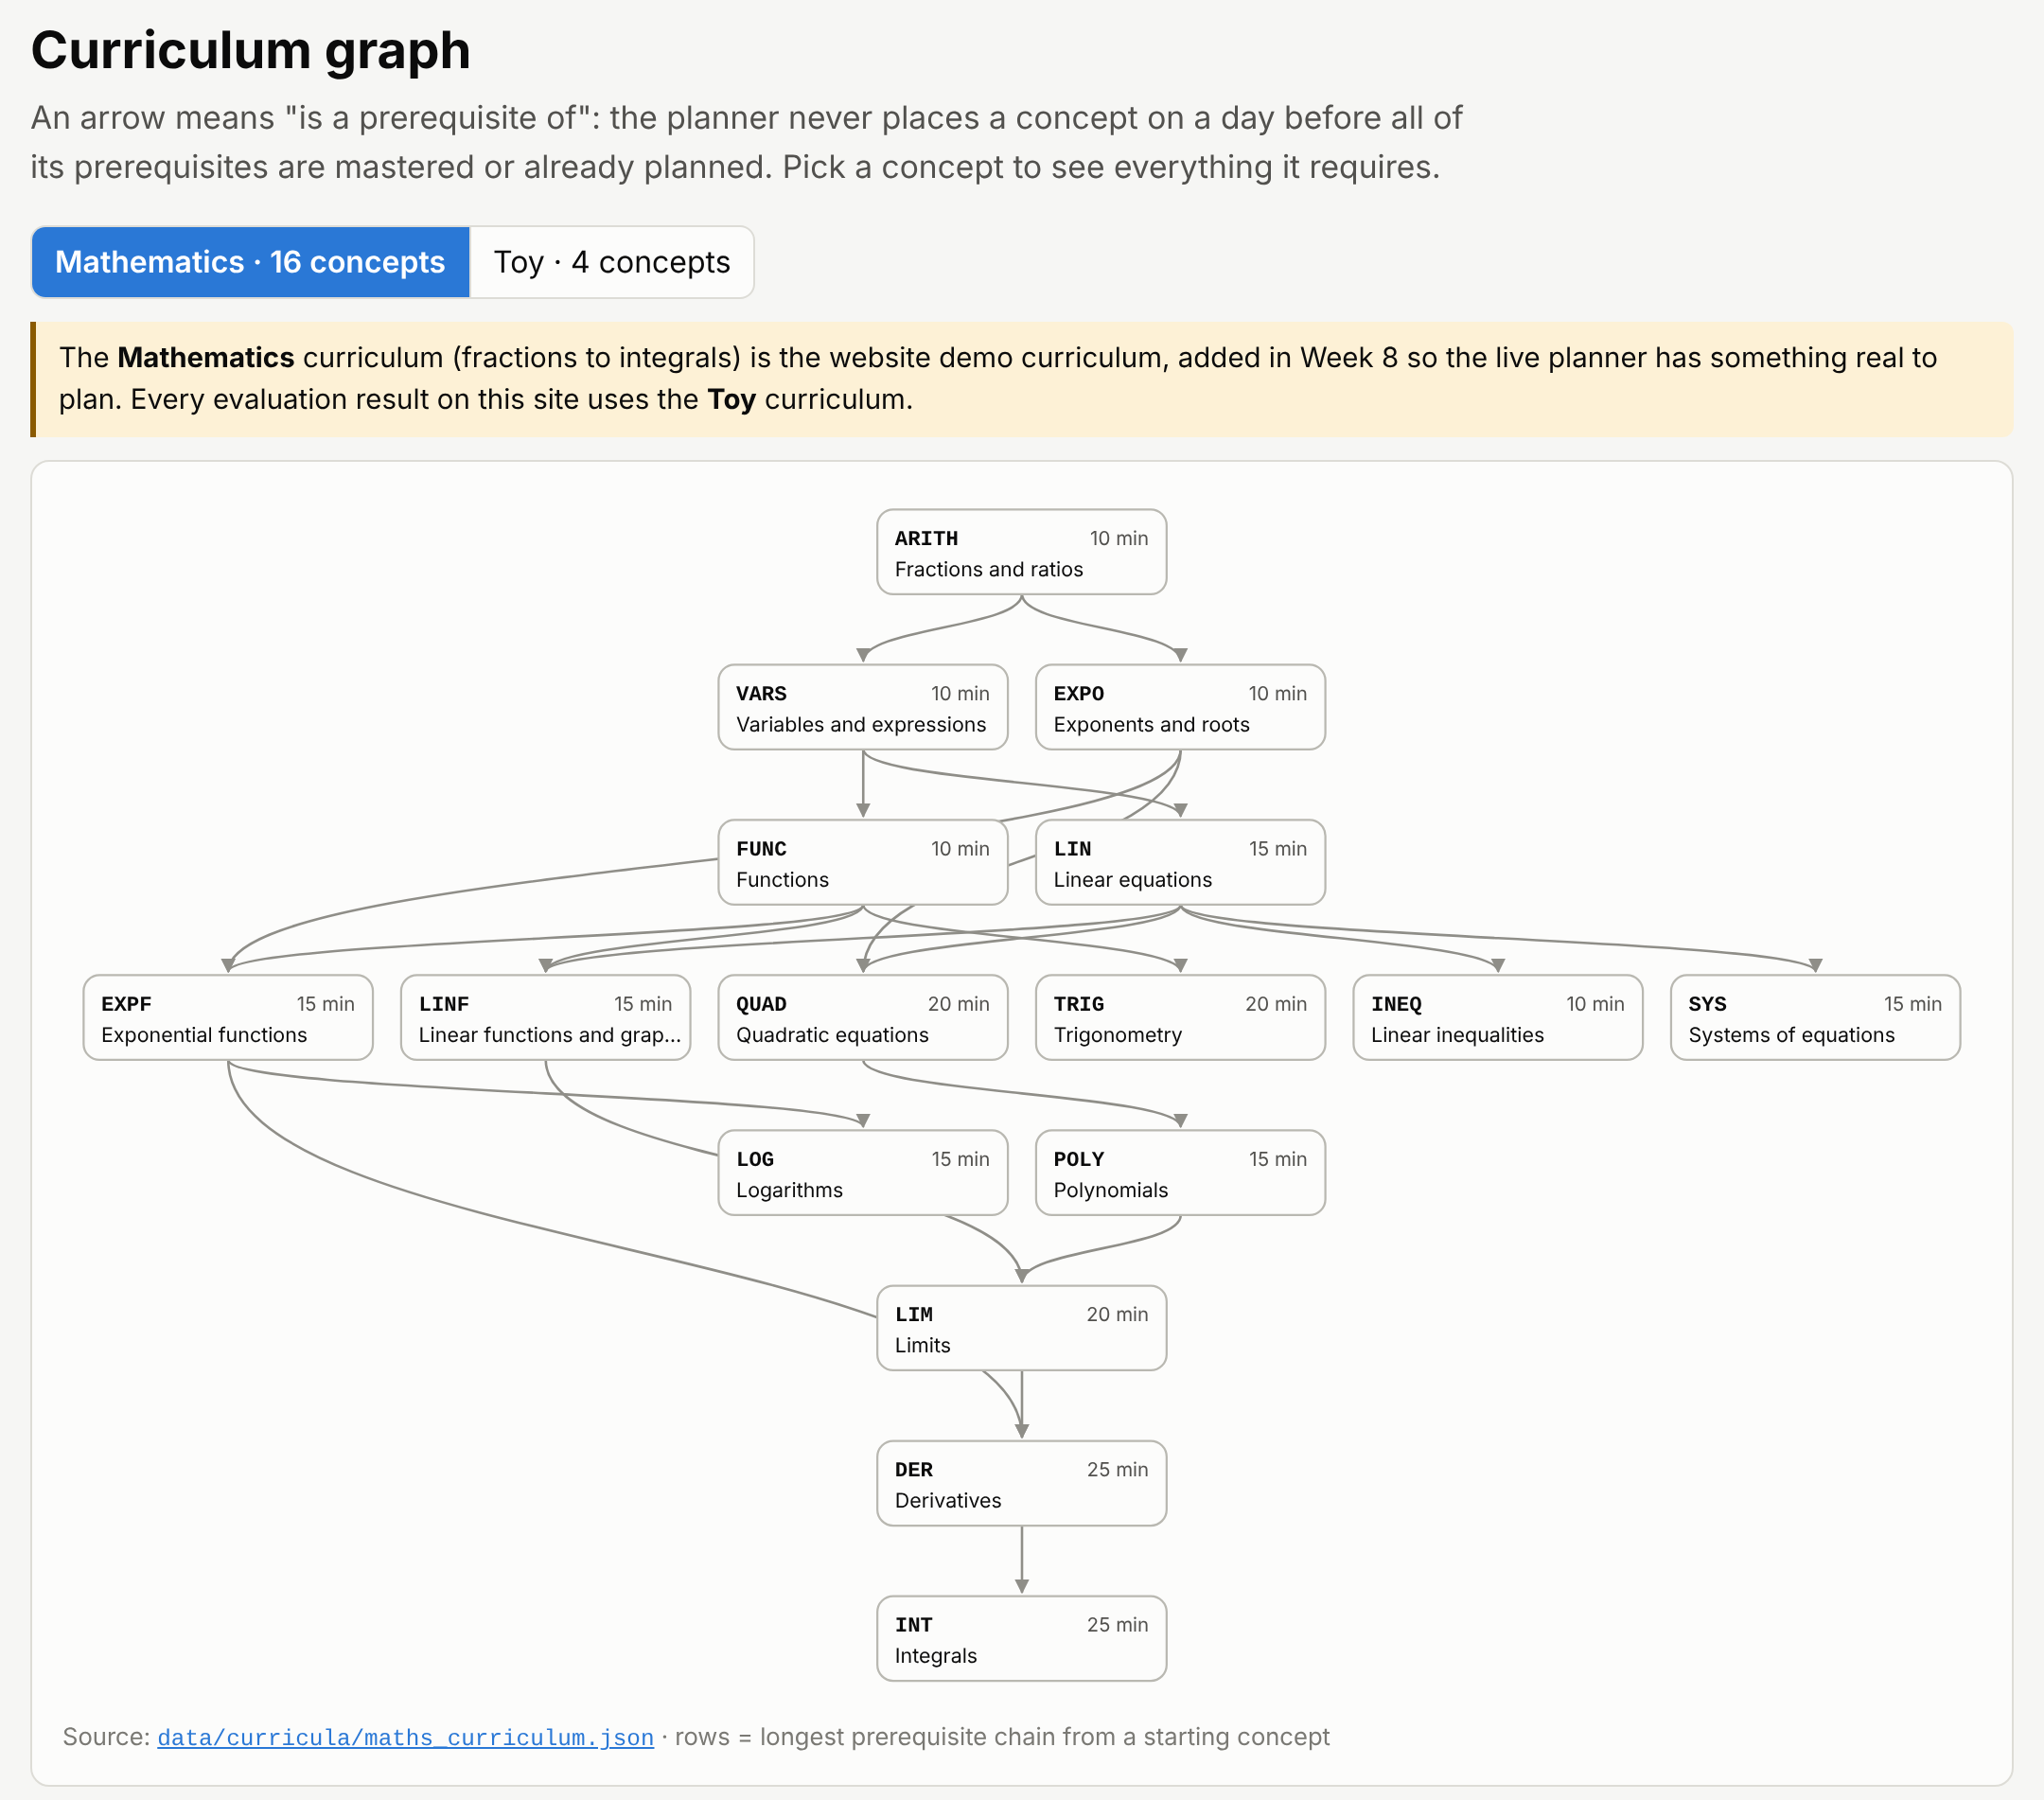
\includegraphics[width=0.78\textwidth]{images/ui_curriculum.png}
    \caption{Curriculum page: the 16-concept maths DAG with durations; clicking a concept highlights its prerequisites.}
\end{figure}
\begin{figure}[H]
    \centering
    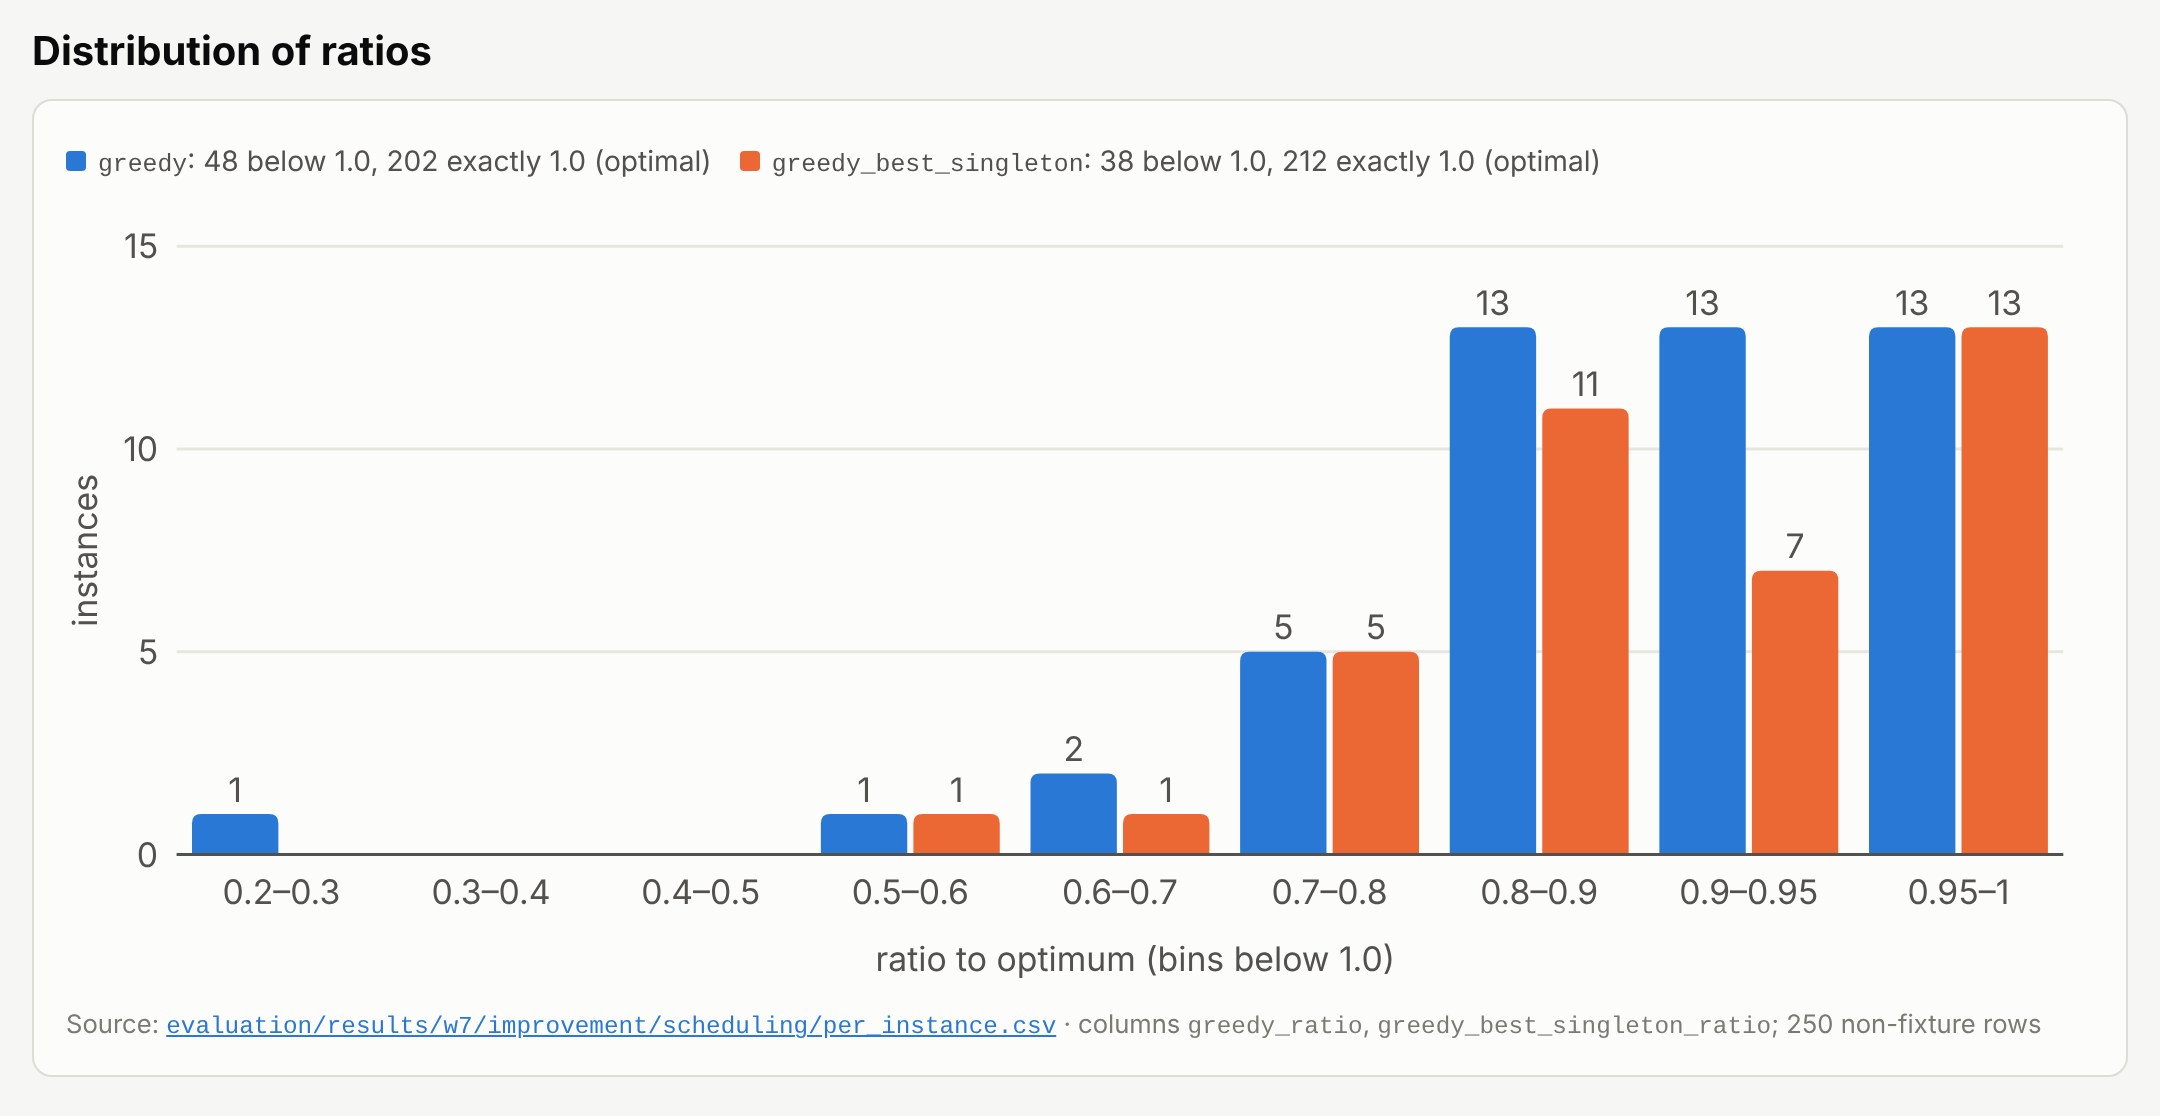
\includegraphics[width=0.88\textwidth]{images/ui_scheduling.png}
    \caption{Scheduling benchmark page: distribution of greedy and best-singleton ratios over 250 instances.}
\end{figure}
\begin{figure}[H]
    \centering
    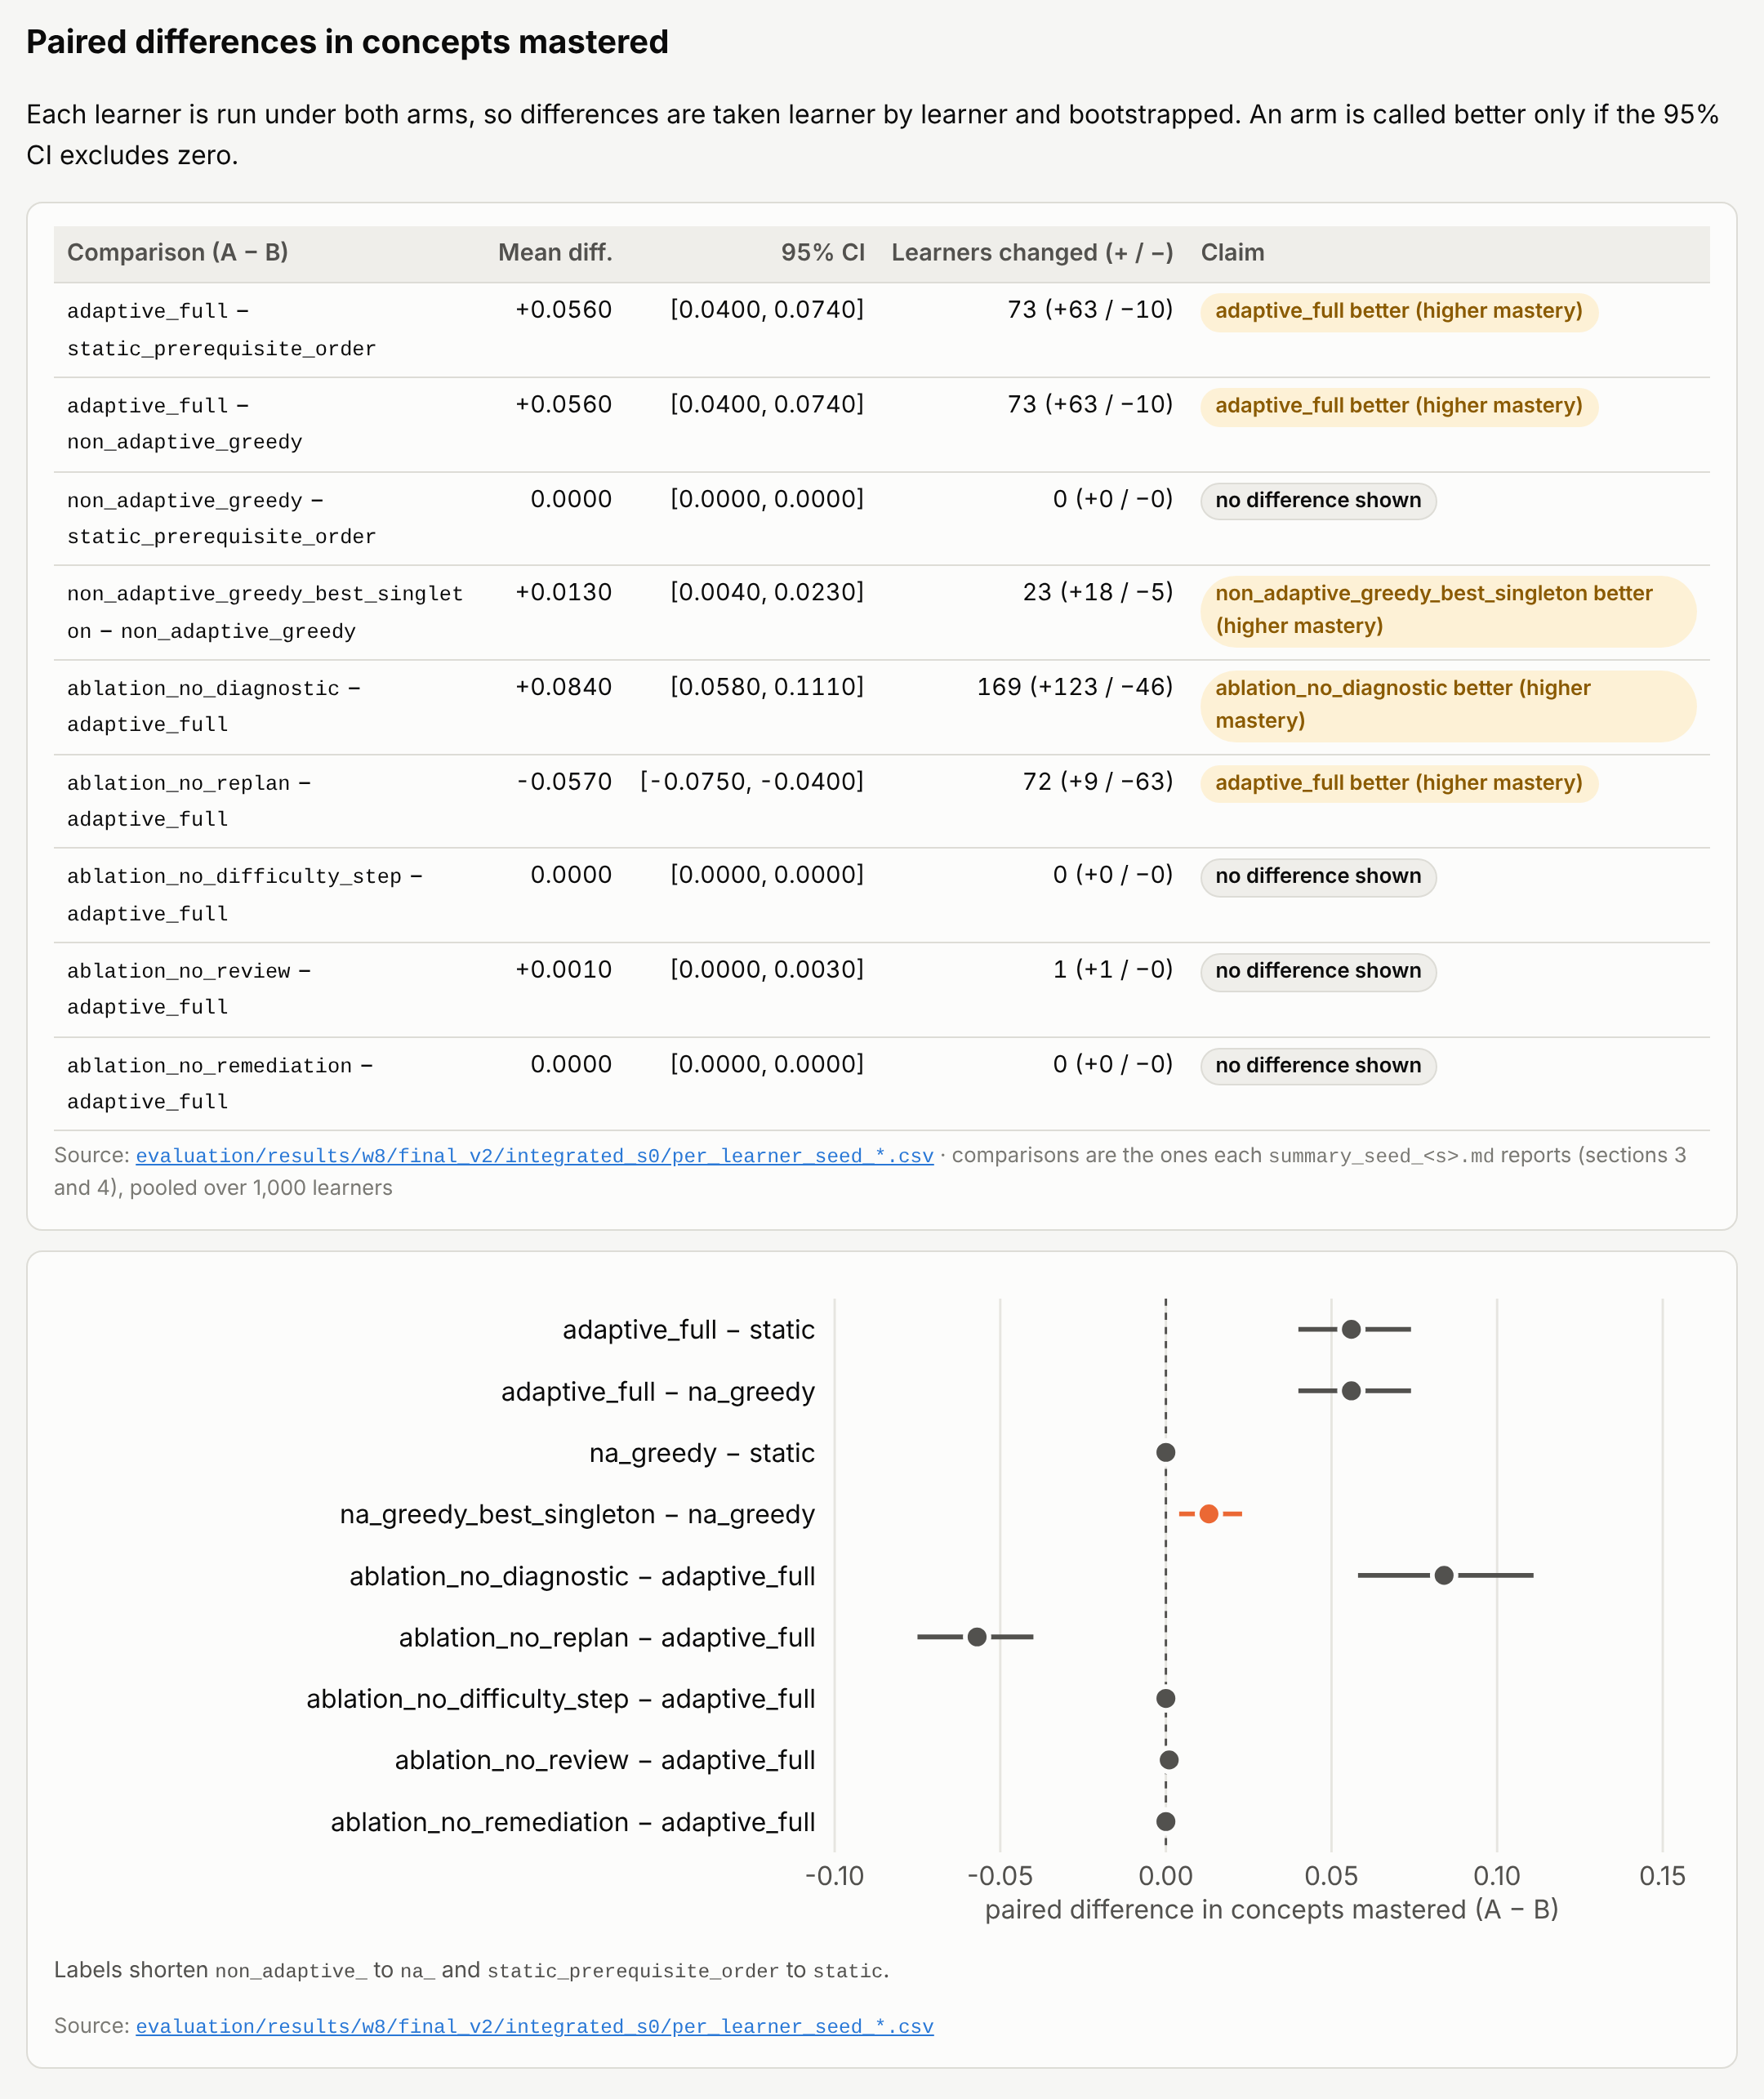
\includegraphics[width=0.88\textwidth]{images/ui_results.png}
    \caption{Results page: paired differences in concepts mastered for S0, with the claim for each comparison.}
\end{figure}
\begin{figure}[H]
    \centering
    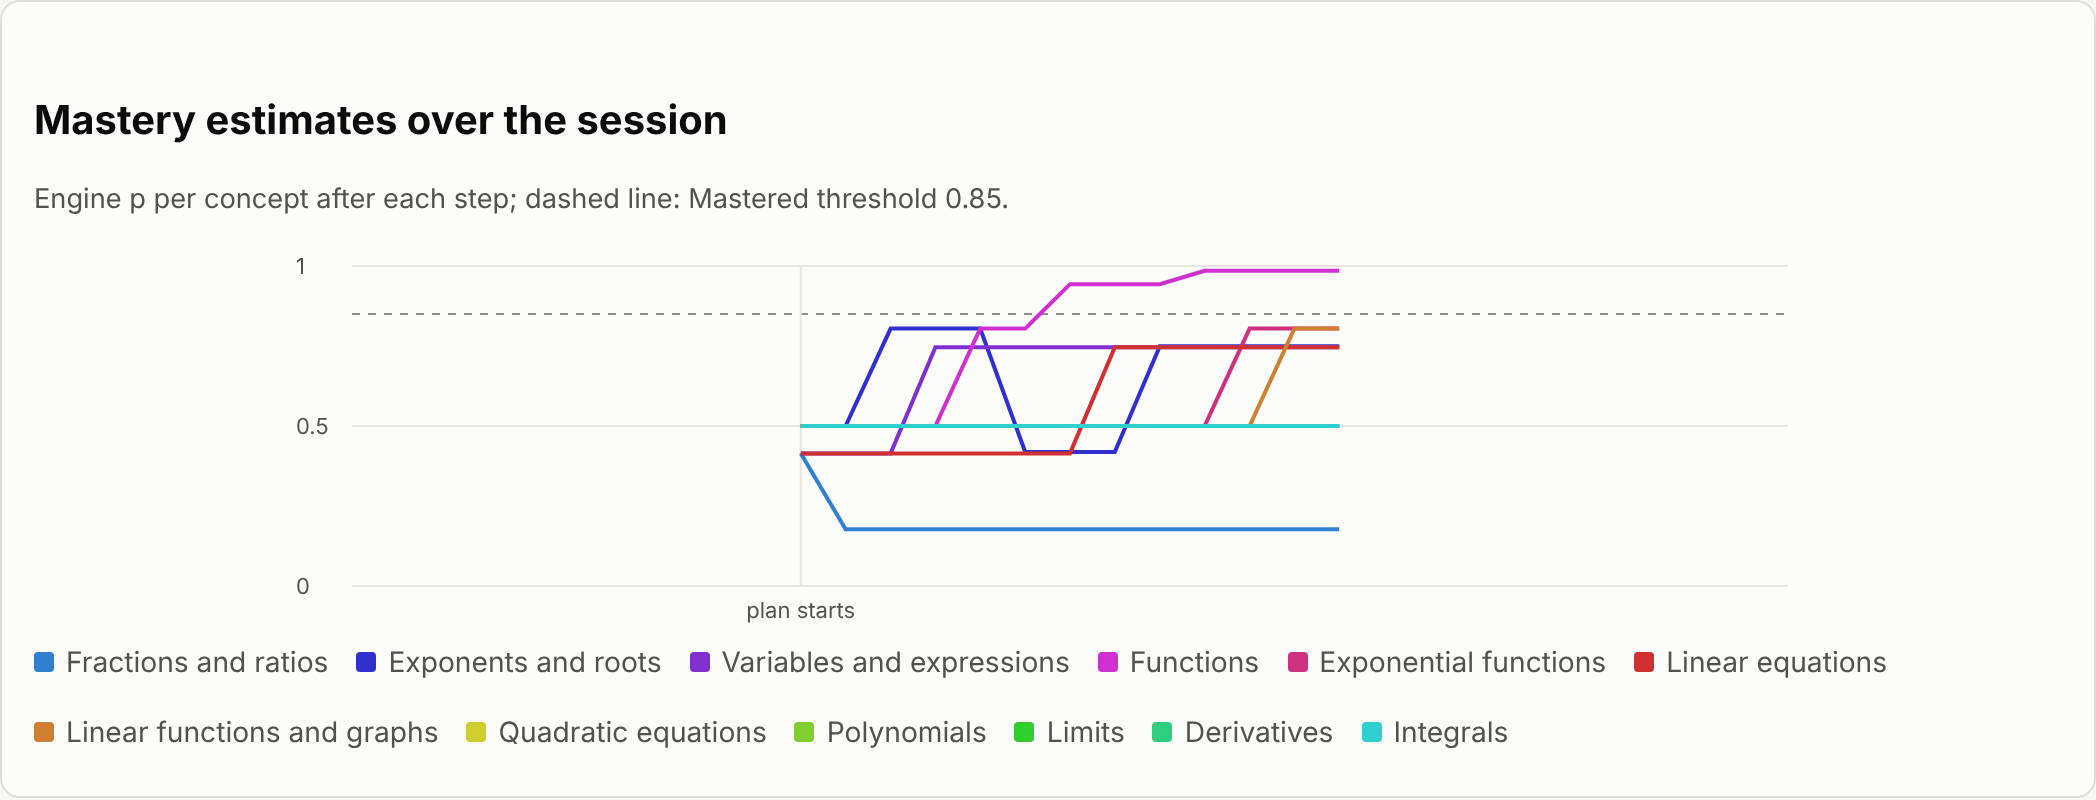
\includegraphics[width=0.88\textwidth]{images/ui_sim_chart.png}
    \caption{Simulation page: the engine's mastery estimate for each of the 12 concepts on the path to Integrals after every step of a recorded run; the dashed line is the Mastered threshold 0.85.}
\end{figure}

\section{Reproduction and Evidence Links}
{\sloppy
All at the final tag \texttt{cs5903-final-2026}. Final report and limitations: \rf{docs/final/FINAL_REPORT.md}, \rf{docs/final/LIMITATIONS.md}. Demo script: \rf{docs/final/DEMO.md}. Formal models and metrics: \rf{docs/FORMAL_MODELS.md}, \rf{docs/METRICS.md}. Acceptance groups: \rf{docs/ACCEPTANCE_GROUPS.md}. Decisions: \rd{decisions}. Weekly records: \rd{weekly}. Raw results: \rd{evaluation/results}; final runs \rd{evaluation/results/w8/final_v2}; diagnostic comparison \rd{evaluation/results/w8/diagnostic_comparison}. Before and after evidence: \rd{evaluation/results/w8_evidence}. Week 8 extension (at \cm{\shax}): \rfx{docs/w8/results_assistments.md}, \rfx{data/provenance/assistments_2009_2010.json}, \rdx{evaluation/results/w8/assistments_bkt}, \rdx{evaluation/results/w8/final_v2/integrated_s4}, \rfx{evaluation/results/w8_evidence/b14_planned_reviews.txt}, \rfx{site/sim.html}, \rfx{site/live.html}. Website source: \rd{site}; live site \href{\siteurl}{\nolinkurl{bhuvan-56.github.io/adaptive-learning-path-planner-DAT/site/}}.

No optional bonus (BP-ID) claims are made.\par}

\end{document}
